
\documentclass[energies,article,submit,moreauthors,noheaderline]{Definitions/mdpi}


\firstpage{1}
\makeatletter
\setcounter{page}{\@firstpage}
\makeatother
\pubvolume{1}
\issuenum{1}
\articlenumber{0}
\pubyear{2026}
\copyrightyear{2026}
\datereceived{ }
\daterevised{ }
\dateaccepted{ }
\datepublished{ }

% Additional packages and local commands used by the converted manuscript.
\usepackage{adjustbox}
\usepackage{makecell}
\usepackage{longtable}
% Compensate for fancyhdr header height warning.
\setlength{\headheight}{20.0pt}
\addtolength{\topmargin}{-8.0pt}
\makeatletter
\def\LT@output{%
  \ifnum\outputpenalty <-\@Mi
    \ifnum\outputpenalty > -\LT@end@pen
      \LT@err{floats and marginpars not allowed in a longtable}\@ehc
    \else
      \setbox\z@\vbox{\unvbox\@cclv}%
      \ifdim \ht\LT@lastfoot>\ht\LT@foot
        \dimen@\pagegoal
        \advance\dimen@-\ht\LT@lastfoot
        \ifdim\dimen@<\ht\z@
          \setbox\@cclv\vbox{\unvbox\z@\copy\LT@foot\vss}%
          \@makecol
          \@outputpage
          \setbox\@cclv\vbox{\box\LT@head}%
        \fi
      \fi
      \global\@colroom\@colht
      \global\vsize\@colht
      \vbox
        {\unvbox\z@\box\LT@foot}%
    \fi
  \else
    \setbox\@cclv\vbox{\unvbox\@cclv\copy\LT@foot\vss}%
    \@makecol
    \@outputpage
    \global\vsize\@colroom
    \copy\LT@head\nobreak
  \fi}
\makeatother
\newcommand{\degree}{\texorpdfstring{\ensuremath{^\circ}}{\textdegree}}

% Strip math tokens from PDF metadata strings (abstract/title) to avoid
% hyperref "Token not allowed in a PDF string" warnings.
\makeatletter
\AtBeginDocument{%
  \pdfstringdefDisableCommands{%
    \def\ensuremath#1{}%
    \def\textsuperscript#1{#1}%
    \def\textsubscript#1{#1}%
    \def\degree{\textdegree}%
    \def\,{ }%
    \def\thinspace{ }%
    \def\quad{ }%
    \def\geq{>=}%
    \def\leq{<=}%
  }%
}
\makeatother

\Title{Parametric Thermo-Hydraulic Benchmarking of Capsule and Dimple Plate Heat Exchanger Channels via Periodic Unit-Cell CFD}

\Author{Cheuk Sing Cheung \textsuperscript{1}, Christos Skarakis \textsuperscript{1} , Lance Smith \textsuperscript{2}, Jiyuan Tu \textsuperscript{1}, Abhijit Date \textsuperscript{1}, Kiao Inthavong \textsuperscript{1} and Sara Vahaji \textsuperscript{1}}

\AuthorNames{Cheuk Sing Cheung, Christos Skarakis, Sara Vahaji, Lance Smith and Kiao Inthavong}

% Affiliations / Addresses
\address{%
\textsuperscript{1} \quad School of Engineering, RMIT University, Melbourne, VIC 3000, Australia\\
\textsuperscript{2} \quad InKorr Pty Ltd, Knoxfield, VIC 3180, Australia}

% Contact information of the corresponding author
\corres{Correspondence: kiao.inthavong@rmit.edu.au}

% Abstract (single paragraph)
\abstract{Plate heat exchangers are widely utilized due to their compact footprint and superior thermal performance. While capsule- and dimple-type embossing surfaces represent recent advancements in plate design, direct comparison on their efficiency remains challenging. Existing literature use different fluids, domains, boundary conditions, and performance definitions. This study benchmarks both surfaces under common conditions to assess how embossing angle and height alter heat transfer relative to flow resistance. Steady-state, single-phase Reynolds-averaged Navier--Stokes simulations cover 28 one-factor periodic-unit-cell cases---seven for each of \texorpdfstring{$\theta_c$, $h_c$, $h_d$, and $\theta_d$}{theta c, h c, h d, and theta d}---and one targeted combined dimple case. Nusselt number measures heat transfer, while the friction factor measures resistance. The performance evaluation criterion (\texorpdfstring{$\mathrm{PEC}=\mathrm{Nu}/f^{1/3}$}{PEC = Nu divided by the cube root of f}) combines these outcomes, so higher PEC indicates a better heat-transfer--friction trade-off; relative embossing depth (\texorpdfstring{$\mathrm{RED}=h/D_e$}{RED = h/De}) normalizes embossing height to channel size. Capsule angle produced the narrowest PEC range (244.4--254.8), whereas capsule height gave the two highest values: 277.1 at \texorpdfstring{$h_c=5.0$~mm}{h c = 5.0 mm} and 273.1 at \texorpdfstring{$h_c=4.5$~mm}{h c = 4.5 mm}. Dimple angle and height covered 219.8--255.1 and 186.8--237.6, respectively. Combining \texorpdfstring{$\theta_d=45\degree$ with $h_d=5.0$~mm}{theta d = 45 degrees with h d = 5.0 mm} raised PEC to 271.5, the best tested dimple case and third overall. The results apply only to the tested geometry and conditions and do not establish a global optimum.}

% Keywords
\keyword{CFD; plate heat exchangers; capsule-type PHE; dimple-type PHE; heat transfer; performance evaluation criterion}

\begin{document}

% Center body pages for local review without editing the MDPI class file.
\newgeometry{left=2.5cm,right=2.5cm,top=2.0cm,bottom=2.0cm,includehead,includefoot}
\fancyheadoffset[L]{0pt}
\fancyfootoffset[L]{0pt}

\begin{table}[H]
\caption{Nomenclature}
\centering
\scriptsize
\renewcommand{\arraystretch}{1.05}
\begin{tabularx}{\textwidth}{@{}l>{\raggedright\arraybackslash}X@{\quad}l>{\raggedright\arraybackslash}X@{}}
\hline
\textbf{Symbol} & \textbf{Description} & \textbf{Symbol} & \textbf{Description} \\
\hline
$A$         & Cross-sectional flow area (mm$^2$) & Nu          & Nusselt number (--) \\
$A_0$       & Minimum flow area; equal to the inlet area (mm$^2$) & $P$ & Wetted perimeter (mm) \\
$C$         & Unit-cell centre & PEC & Performance evaluation criterion (--) \\
$C_p$       & Specific heat capacity (J/kg$\cdot$K) & Pr          & Prandtl number (--) \\
$D$         & Dimple diameter (mm) & $Q$ & Heat-transfer rate (W) \\
$D_e$       & Hydraulic diameter (mm) & Re          & Reynolds number (--) \\
$f$         & Friction factor (--) & $\mathrm{Re}_x$ & Local Reynolds number (--) \\
$h$         & Embossing height (mm) & RED         & Relative Embossing Depth (--) \\
$h_{ave}$   & Average heat-transfer coefficient (W/m$^2\cdot$K) & $S$         & Total heat-transfer area (mm$^2$) \\
$h_c$       & Capsule height (mm) & $T_{f,ave}$ & Average fluid temperature (K) \\
$h_d$       & Dimple height (mm) & $T_{f,in}$ & Fluid inlet temperature (K) \\
$k$         & Turbulence kinetic energy (m$^2$/s$^2$) & $T_{f,out}$ & Fluid outlet temperature (K) \\
$l$         & Capsule length (mm)  & $T_w$       & Wall temperature (K) \\
$l_c$       & Capsule unit-cell length (mm) & $u$         & Inlet velocity (m/s) \\
$l_d$       & Dimple unit-cell length (mm) & $w$         & Capsule width (mm) \\
$\dot{m}$         & Mass flow rate (kg/s) & $x$         & Streamwise distance (m) \\
            &                       & $y^+$       & Dimensionless wall distance (--) \\
\hline
\multicolumn{2}{l}{\textbf{Greek symbols}} & \multicolumn{2}{l}{\textbf{Abbreviations}} \\
\hline
$\delta$    & Boundary-layer thickness (m) & CFD   & Computational fluid dynamics \\
$\Delta p$  & Pressure drop (Pa) & CPHE  & Capsule-type plate heat exchanger \\
$\Delta\mathrm{PEC}$ & Difference between matched CPHE and DPHE PEC values (--) & & \\
$\epsilon$  & Turbulence dissipation rate (m$^2$/s$^3$) & DPHE  & Dimple-type plate heat exchanger \\
$\theta_c$  & Capsule angle (\degree) & HVAC  & Heating, ventilation, and air-conditioning \\
$\theta_d$  & Dimple angle (\degree) & PHE   & Plate heat exchanger \\
$\lambda$   & Thermal conductivity (W/m$\cdot$K) & RANS  & Reynolds-averaged Navier--Stokes \\
$\rho$      & Fluid density (kg/m$^3$) & SST   & Shear Stress Transport \\
$\upsilon$  & Kinematic viscosity (m$^2$/s) & STHE  & Shell-and-tube heat exchanger \\
$\omega$    & Specific dissipation rate (s$^{-1}$) & TKE   & Turbulence kinetic energy \\          
\hline
\end{tabularx}
\end{table}


\section{Introduction}
\label{sec:introduction} 


Plate heat exchangers (PHEs) place a large heat-transfer area within a compact volume and are widely used in power generation, process industries, heating and cooling systems, and refrigeration. Alternating embossed plates form narrow passages that repeatedly disturb the thermal and hydrodynamic boundary layers. This disturbance can strengthen convection and reduce the area required for a specified thermal duty, but the associated separation, recirculation, and wall shear also increase pressure loss and pumping demand. Heat transfer and hydraulic resistance are therefore coupled design objectives: an embossing should not be judged by Nusselt number alone if its thermal gain is obtained at a disproportionate friction penalty \citep{abukhader2012, thulukkanam2013, zhang2019a}. Although chevron plates remain the conventional reference, capsule, dimple, and pillow surfaces provide alternative ways to control the flow path and surface-area distribution.

The capsule studies summarized in Table~\ref{tab:embossing-summary} demonstrate that performance depends on more than the presence of an embossing. \citet{hamedi2024} reported that a symmetric convex--concave capsule arrangement increased Nusselt number by 28--55\% relative to a simple channel, but also increased the friction factor by 35--44\%. Capsule aspect ratio and size further shift this balance: a larger length-to-width ratio can improve energy efficiency, whereas smaller capsules intensify heat transfer and pressure loss \citep{jiang2019a, jiang2020}. Symmetric arrangements have outperformed zig-zag layouts, and capsule surfaces have also produced higher Nusselt numbers with lower friction factors than chevron surfaces under the conditions examined by \citet{zhang2016}. Geometry optimization produced an 8.3\% increase in heat-transfer coefficient together with a 14.3\% reduction in friction \citep{yu2024}, while adding secondary dimples to capsule surfaces increased heat transfer by 19--46\% \citep{shao2024}. Collectively, these results show that capsule orientation, size, aspect ratio, and arrangement can reorganize the thermal--hydraulic trade-off; they do not identify one configuration that remains superior under a different geometry or operating basis.

The dimple and pillow literature shows the same sensitivity to geometry. Pillow plates have required 30\% less heat-transfer area than chevron plates while producing a lower pressure drop \citep{arsenyeva2019}, and a dimpled pillow channel achieved an 11.2\% thermo-hydraulic improvement with an 8.7\% pressure-loss reduction \citep{piper2019}. For standalone dimple surfaces, \citet{soman2022} reported a 39\% Nusselt-number increase relative to a flat PHE, while hemispherical dimples produced a heat-transfer coefficient approximately 27.2\% higher than rhombus dimples \citep{ying2021}. Numerical predictions have also been compared with experiments for several dimple channels, including deviations of $-11\%$ to 1.8\% in one study series \citep{mocnik2020, mocnik2023, mocnik2024}. Other investigations considered supercritical CO$_2$, nanofluids, lubricating oil, two-phase flow, or hybrid capsule--dimple plates \citep{jing2019, li2019, soman2019, torre2019, shao2024}. These results confirm that dimple shape, channel configuration, and working fluid all influence the balance between heat transfer and pressure loss.

Table~\ref{tab:embossing-summary} thus provides strong evidence for both embossing families, but it also exposes the comparison gap. The reported studies use different fluids, Reynolds-number ranges, channel domains, boundary conditions, hydraulic-diameter definitions, turbulence models, reference surfaces, and performance measures. Some investigate single-phase water, whereas others consider nanofluids, supercritical fluids, or multiphase flow; some report Nusselt number and friction factor separately, whereas others use a combined thermo-hydraulic index. Consequently, the published percentage improvements cannot be ranked on a common scale. Most studies also vary parameters within one surface family, leaving it unclear whether the performance of CPHE and DPHE channels responds similarly when angle and height are changed over comparable ranges.

A controlled computational fluid dynamics (CFD) study is suitable for resolving this gap because it provides both integral performance measures and spatial evidence of the mechanisms that produce them. Nusselt number and pressure loss quantify the overall thermal and hydraulic response, while turbulence kinetic energy, streamlines, and temperature fields reveal how an embossing redirects flow, forms wakes, and transports heat from the wall to the channel core. Periodic unit cells have been used successfully for repeating capsule and dimple geometries because they retain the local embossing-induced mechanisms while avoiding the cost of modelling an entire exchanger \citep{hamedi2024, jiang2019a, jiang2020, piper2019, shao2024}. Published comparisons with experiments also support the use of steady RANS modelling for this class of channel \citep{mocnik2020, mocnik2023, mocnik2024}. The SST $k$--$\omega$ model is selected because its near-wall treatment and response to adverse pressure gradients are suited to the separated flows produced by embossed passages \citep{kanaris2006, menter1994}.

The present study therefore benchmarks capsule-type plate heat exchanger (CPHE) and dimple-type plate heat exchanger (DPHE) channels within one steady-state, single-phase water-flow RANS framework at $\mathrm{Re}=4282$. Both geometries use a periodic unit cell, common thermal and hydraulic boundary conditions, and the same hydraulic-diameter definition, so the effects of geometry are not obscured by a change in the numerical basis. Twenty-eight one-factor cases comprise four seven-case sweeps. Capsule and dimple angles cover $0\degree$--$45\degree$ in $7.5\degree$ increments, while capsule and dimple heights cover 2.0--5.0~mm in 0.5~mm increments; the remaining geometric variables are held at the reference values listed in Table~\ref{tab:geom_cases}. This design separates the effects of capsule angle ($\theta_c$), capsule height ($h_c$), dimple height ($h_d$), and dimple flow-entry angle ($\theta_d$). One additional case combines $\theta_d=45\degree$ with $h_d=5.0$~mm to test a targeted dimple interaction identified from the one-factor results, rather than treating the four sweeps as a full factorial optimization.

The study has three objectives: to quantify how the four geometric variables change Nusselt number and the friction factor; to explain those changes using the computed flow and temperature fields; and to compare CPHE and DPHE cases through the performance evaluation criterion (PEC) and relative embossing depth (RED). PEC expresses the heat-transfer--friction trade-off on a common scale, while RED relates embossing height to the effective channel size. This common framework permits a direct benchmark that the heterogeneous literature cannot provide. The finite sweeps and single combined case nevertheless support conclusions only for the tested geometry, fluid, Reynolds number, and boundary conditions; they do not establish a global optimum across untested parameter interactions.

{\footnotesize
\setlength{\LTleft}{0pt}
\setlength{\LTright}{0pt}
\setlength{\LTpre}{0pt}
\setlength{\LTpost}{0pt}
\begin{longtable}{@{}>{\raggedright}p{2.6cm} >{\raggedright}p{1.6cm} >{\raggedright}p{1.6cm} >{\raggedright\arraybackslash}p{8.9cm}@{}}
\caption{Summary of embossing surface enhancement of PHEs}
\label{tab:embossing-summary} \\
\hline
\textbf{Author} & \textbf{Surface} & \textbf{Method\textsuperscript{a}} & \textbf{Key Findings} \\
\hline
\endfirsthead
\caption[]{(continued)} \\
\hline
\textbf{Author} & \textbf{Surface} & \textbf{Method\textsuperscript{a}} & \textbf{Key Findings} \\
\hline
\endhead
\hline
\endfoot
\citet{hamedi2024} & Capsule & E \& N & Proposed a symmetrical arrangement of convex and concave capsule surfaces. Relative to a simple channel, the friction factor increased by 35--44\% and the Nusselt number by 28--55\%. \\
\citet{jiang2019a} & Capsule & N & Found that the capsule length-to-width ratio controls the performance trade-off: a larger ratio improves energy efficiency, while a smaller ratio increases heat transfer and pressure drop. \\
\citet{jiang2020} & Capsule & N & A symmetrical capsule arrangement outperformed a zig-zag arrangement. Smaller capsules increased heat transfer, while larger capsules reduced pressure loss. \\
\citet{jiang2019} & Capsule & E & Found that plate-corrugation geometry had little effect on liquid and gas distribution during two-phase channel flow. \\
\citet{zhang2016} & Capsule & E \& N & Capsule embossing produced a higher Nusselt number and lower friction factor than chevron surfaces. \\
\citet{yu2024} & Capsule & N & Combined CFD with backpropagation optimization, increasing the heat-transfer coefficient by 8.3\% and reducing friction by 14.3\%. \\
\citet{shao2024} & Capsule / Dimple & N & Adding secondary dimples to capsule surfaces increased heat transfer by 19--46\%. \\
\citet{arsenyeva2019} & Pillow & E \& N & Required 30\% less heat-transfer area than chevron plates and produced a lower pressure drop. \\
\citet{shirzad2019a} & Pillow & N & Greater channel height was most efficient at low Reynolds numbers, while wider transverse welding-spot spacing was most efficient at high Reynolds numbers. \\
\citet{shirzad2019b} & Pillow & N & Predicted higher thermal performance with a nanofluid than with water. \\
\citet{kumar2019} & Pillow & N & Numerically examined heat transfer and fluid flow in a pillow-plate channel. \\
\citet{piper2019} & Pillow / Dimple & N & Reported an 11.2\% improvement in thermo-hydraulic performance and an 8.7\% reduction in pressure loss. \\
\citet{jing2019} & Dimple & N & Numerically examined supercritical CO$_2$ flow and heat transfer in rectangular channels with teardrop dimples. \\
\citet{li2019} & Dimple & E & Found that smaller air bubbles produced greater heat transfer than medium or large bubbles during two-phase flow. \\
\citet{mocnik2020} & Dimple & E \& N & Compared turbulence models with experimental data and identified two flow regimes. \\
\citet{mocnik2023} & Dimple & E \& N & Reported numerical results from $-$11\% to 1.8\% relative to the experiments. \\
\citet{mocnik2024} & Dimple & E \& N & Found good agreement between numerical and experimental results for low-Reynolds-number flow in a dimple-type PHE. \\
\citet{soman2019} & Dimple & E & Nanofluids improved heat transfer relative to water without increasing the friction factor. \\
\citet{soman2022} & Dimple & N & A dimple PHE increased the Nusselt number by 39\% relative to a flat PHE. \\
\citet{torre2019} & Dimple & E \& N & Obtained satisfactory agreement between experiments and simulations for pressure drop and heat transfer with lubricating oil. \\
\citet{wang2019} & Dimple & N & A dimpled surface reduced pressure drop by 20.57\% and increased net power generation by 173.6\%. \\
\citet{ying2021} & Dimple & E \& N & Hemispherical dimple channels produced a heat-transfer coefficient about 27.2\% higher than rhombus dimple channels. \\
\hline
\multicolumn{4}{l}{\textsuperscript{a}E -- Experimental; N -- Numerical}
\end{longtable}
}

\section{Methodology}
\label{sec:methodology}

This numerical investigation applies a common computational fluid dynamics (CFD) framework to benchmark the thermo-hydraulic performance of CPHE and DPHE channels. The method combines periodic unit-cell representation, mesh-independence testing, literature-supported turbulence modelling, and controlled parametric sweeps \citep{jiang2019, mocnik2020}.

\subsection{Numerical methods}
\label{sec:numerical_methods}

The Reynolds-averaged Navier--Stokes (RANS) approach is widely used in numerical studies of capsule and dimple channels. Published models include realizable $k$--$\epsilon$ \citep{kumar2019, jing2019, mocnik2020, mocnik2024}, shear stress transport (SST) $k$--$\omega$ \citep{hamedi2024, jiang2019a, jiang2020, mocnik2020, mocnik2024, torre2019}, Reynolds stress \citep{shao2024, mocnik2023}, elliptic-blending $k$--$\epsilon$ \citep{arsenyeva2019, piper2019}, and standard $k$--$\epsilon$ \citep{soman2022}. The SST $k$--$\omega$ model is used here because it combines near-wall $k$--$\omega$ treatment with a $k$--$\epsilon$ formulation away from the wall and is suited to separated flows with adverse pressure gradients \citep{kanaris2006, khail2023, menter1994}.

All simulations use steady-state, single-phase water flow at subcritical pressure and temperature.

Due to the complexity of the geometry of CPHE and DPHE, the local hydraulic diameter varies periodically; the hydraulic diameter calculation below will be adopted to determine the hydraulic diameter $D_e$ of the channel:
\begin{equation}
D_e=\frac{4A_0 l_c}{S}
\label{eq:De}
\end{equation}
where $A_0$ is the minimum flow area (which is the inlet area for all presented cases), $l_c$ is the unit-cell length, and $S$ is the total heat transfer area. Comparing to general formula for hydraulic diameter $\frac{4A}{P}$, this  $D_e$ applies to the unique flow area of the unit cell, which is expanding and contracting across flow cross-sections along the flow length \citep{zohuri2017}, and had been successfully applied in previous studies \citep{jiang2019a, He2013}. The concept of a unit cell will be discussed in the geometry section. Reynolds number Re is defined as follows:
\begin{equation}
\text{Re}=\frac{uD_e}{\upsilon}
\label{eq:Re}
\end{equation}
where $u$ and $\upsilon$ indicate the inlet velocity and kinematic viscosity of the fluid, respectively. Friction factor ($f$) is adopted for this study and is defined as follows:
\begin{equation}
f=\frac{\Delta p \, D_e}{2\rho \, l_c \, u^2}
\label{eq:f}
\end{equation}
where $\rho$ is the fluid density and $\Delta p$ is obtained directly from the converged inlet-to-outlet pressure difference. The no-slip walls are modelled as hydraulically smooth, with a roughness height of 0~mm and no additional roughness model; Equation~\eqref{eq:f} therefore evaluates $f$ from the simulated pressure loss rather than from an empirical roughness-based correlation. Nusselt number Nu and molecular Prandtl number Pr are defined as follows:
\begin{equation}
\text{Q}=\dot{m}C_p (T_{f,out}-T_{f,in}) 
\label{eq:Q}
\end{equation}
\begin{equation}
h_{ave}=\frac{Q}{(T_w - T_{f,ave})S} 
\label{eq:h_ave}
\end{equation}
\begin{equation}
\text{Nu}=\frac{h_{ave} D_e}{\lambda} 
\label{eq:Nu}
\end{equation}
\begin{equation}
\text{Pr}=\frac{\upsilon\rho C_p}{\lambda}
\label{eq:Pr}
\end{equation}
where $Q$ is the heat-transfer rate; $T_w$, $T_{f,out}$, $T_{f,in}$, and $T_{f,ave}$ are the wall, outlet-fluid, inlet-fluid, and average fluid temperatures, respectively. $m$, $h_{ave}$, $C_p$, and $\lambda$ represent the mass flow rate, average heat-transfer coefficient of the plates, specific heat capacity of the fluid, and thermal conductivity of the fluid, respectively.

In this study, the fluid properties ($\lambda$, $\rho$, $\upsilon$, $C_p$) and Reynolds number remain constant as follows: $\lambda = 0.6$~W/m$\cdot$K, $\rho = 998.2$~kg/m$^3$, $\upsilon = 1.00481 \times 10^{-6}$~m$^2$/s, $C_p = 4182$~J/kg$\cdot$K, and $Re=4282$. 

\subsection{Geometry}
\label{sec:geometry}

Two embossed channel families are considered: capsule and dimple. Both use alternating convex and concave features to disturb the flow, but their planform geometry differs.

The periodic surface is represented by its smallest repeating unit cell. This commonly used approach reduces the computational domain while retaining the flow, thermal, and turbulence mechanisms generated by the repeating embossments \citep{hamedi2024,jiang2019,jiang2020, kumar2019, piper2019, shao2024, zhang2016}.

\begin{figure}[!ht]
\centering
\begin{tabular}{cccc}
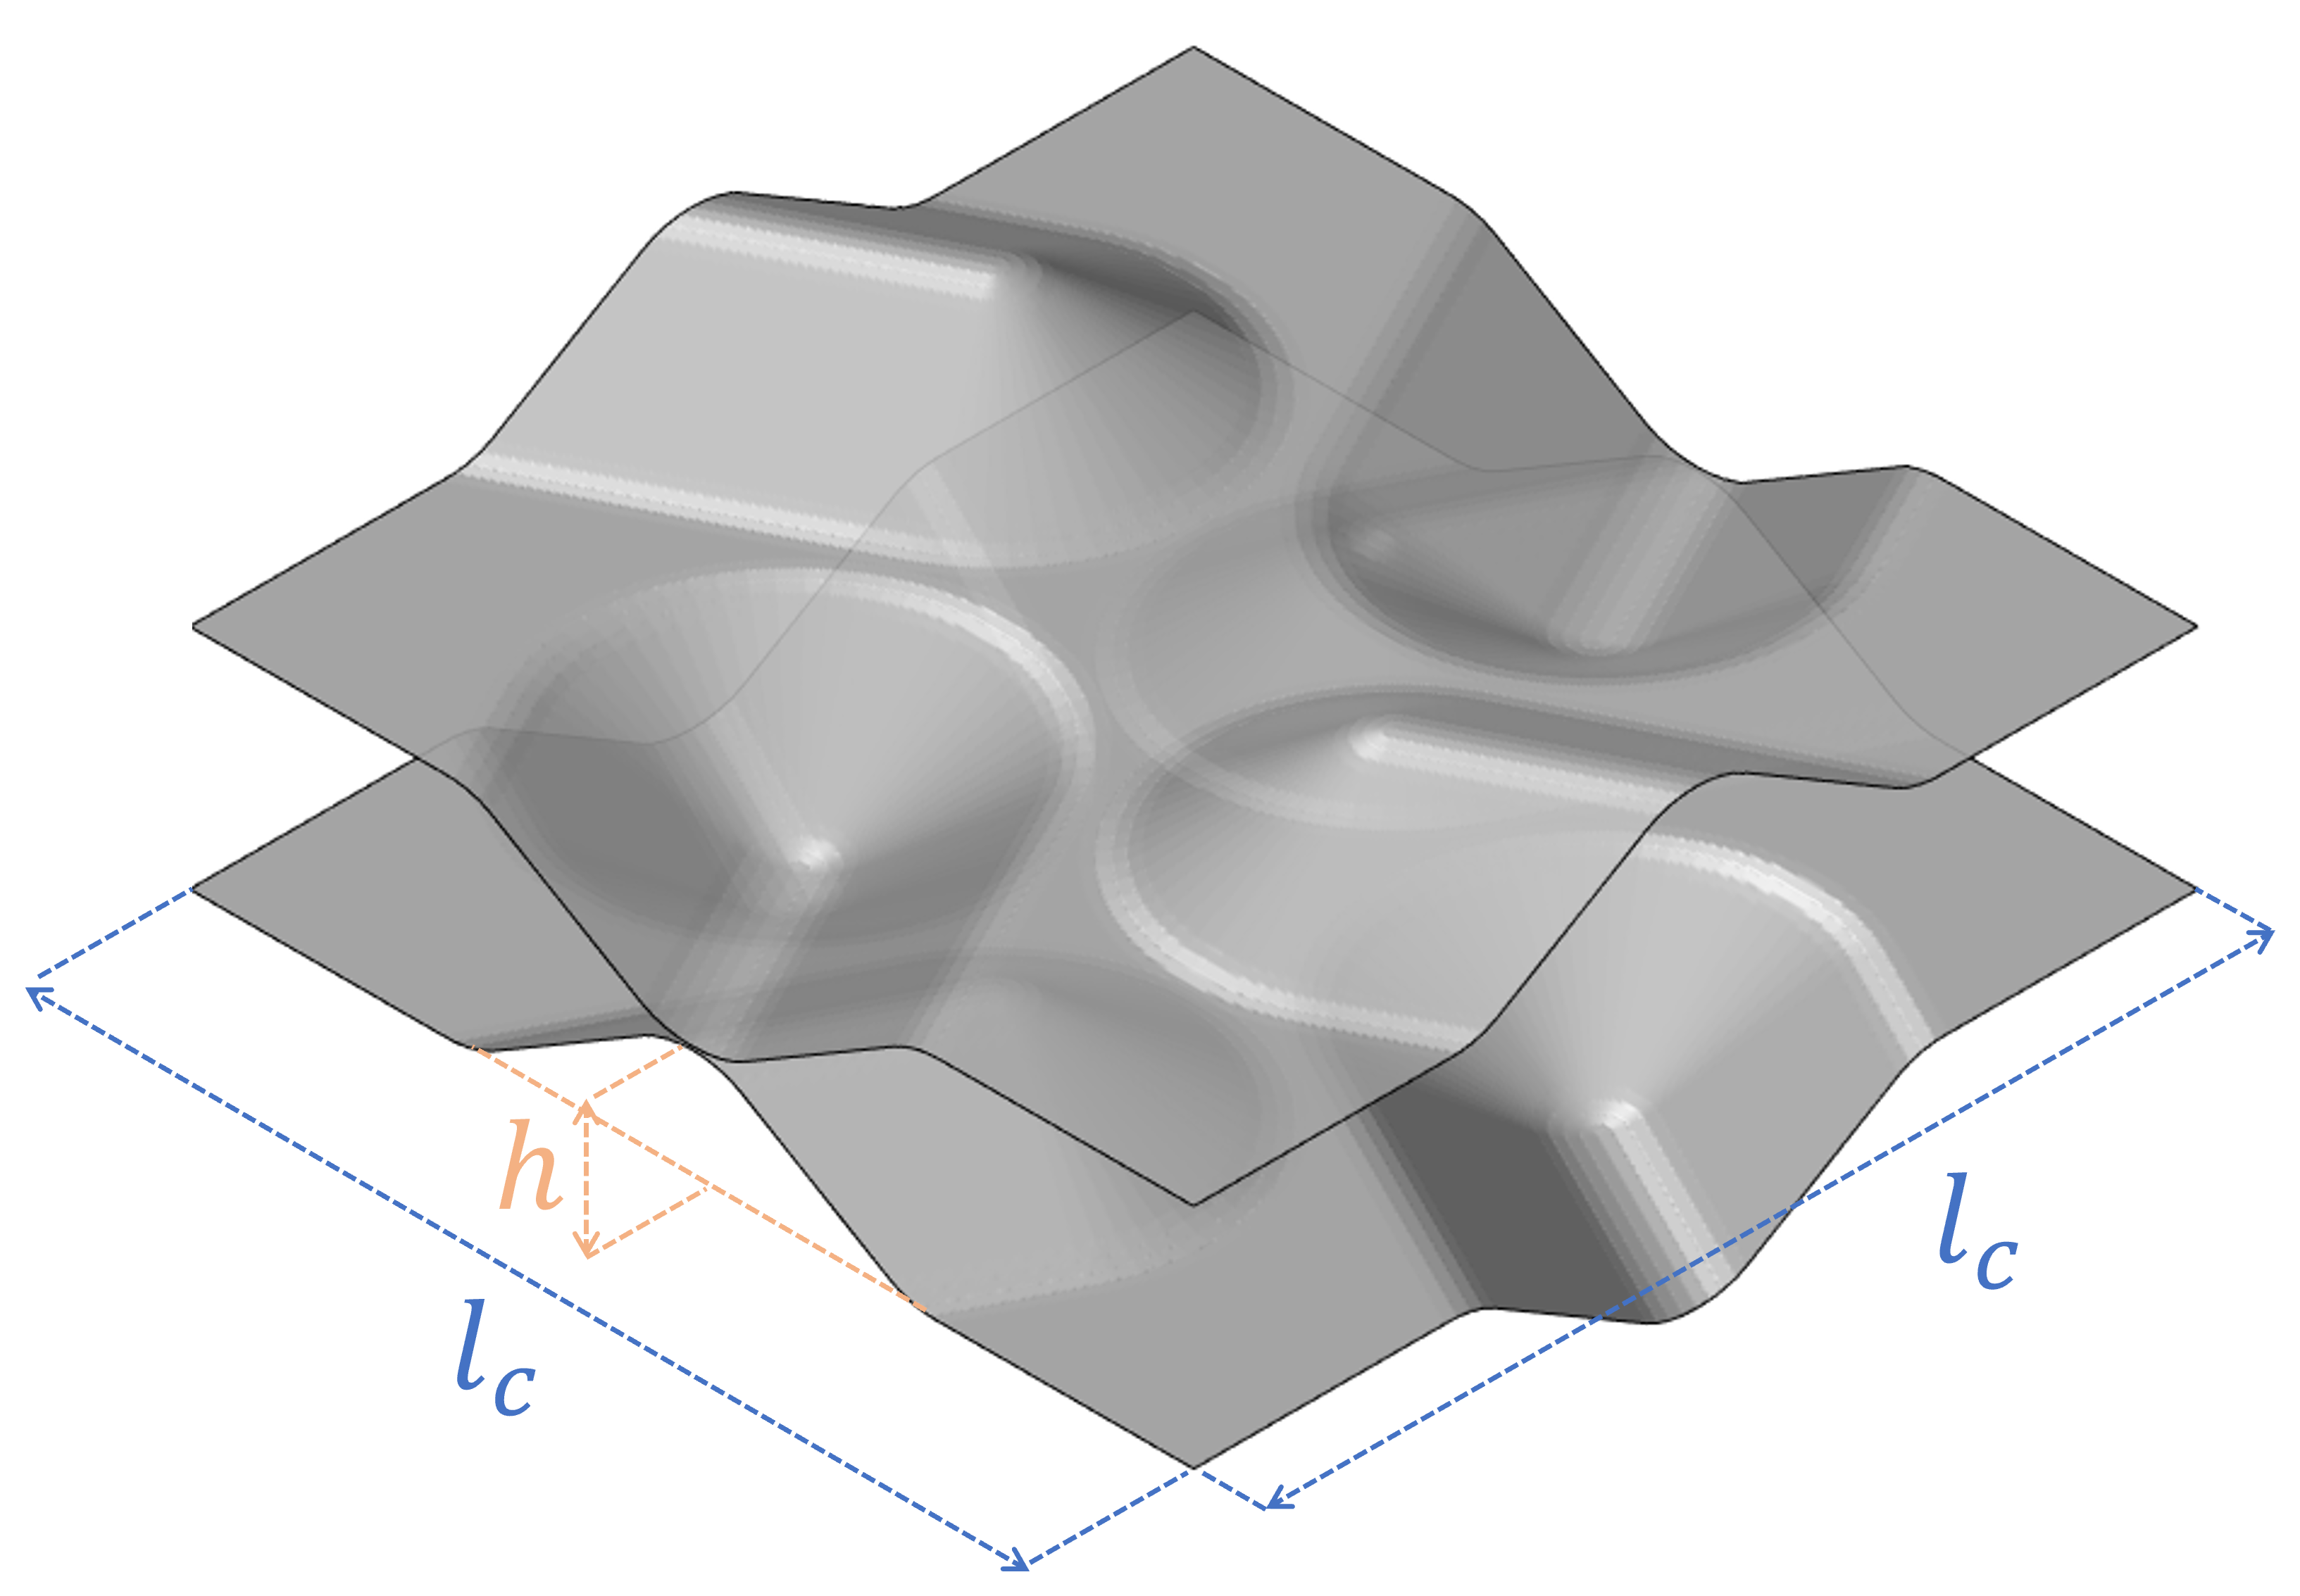
\includegraphics[width=0.3\textwidth]{media/image6_v2.png} &
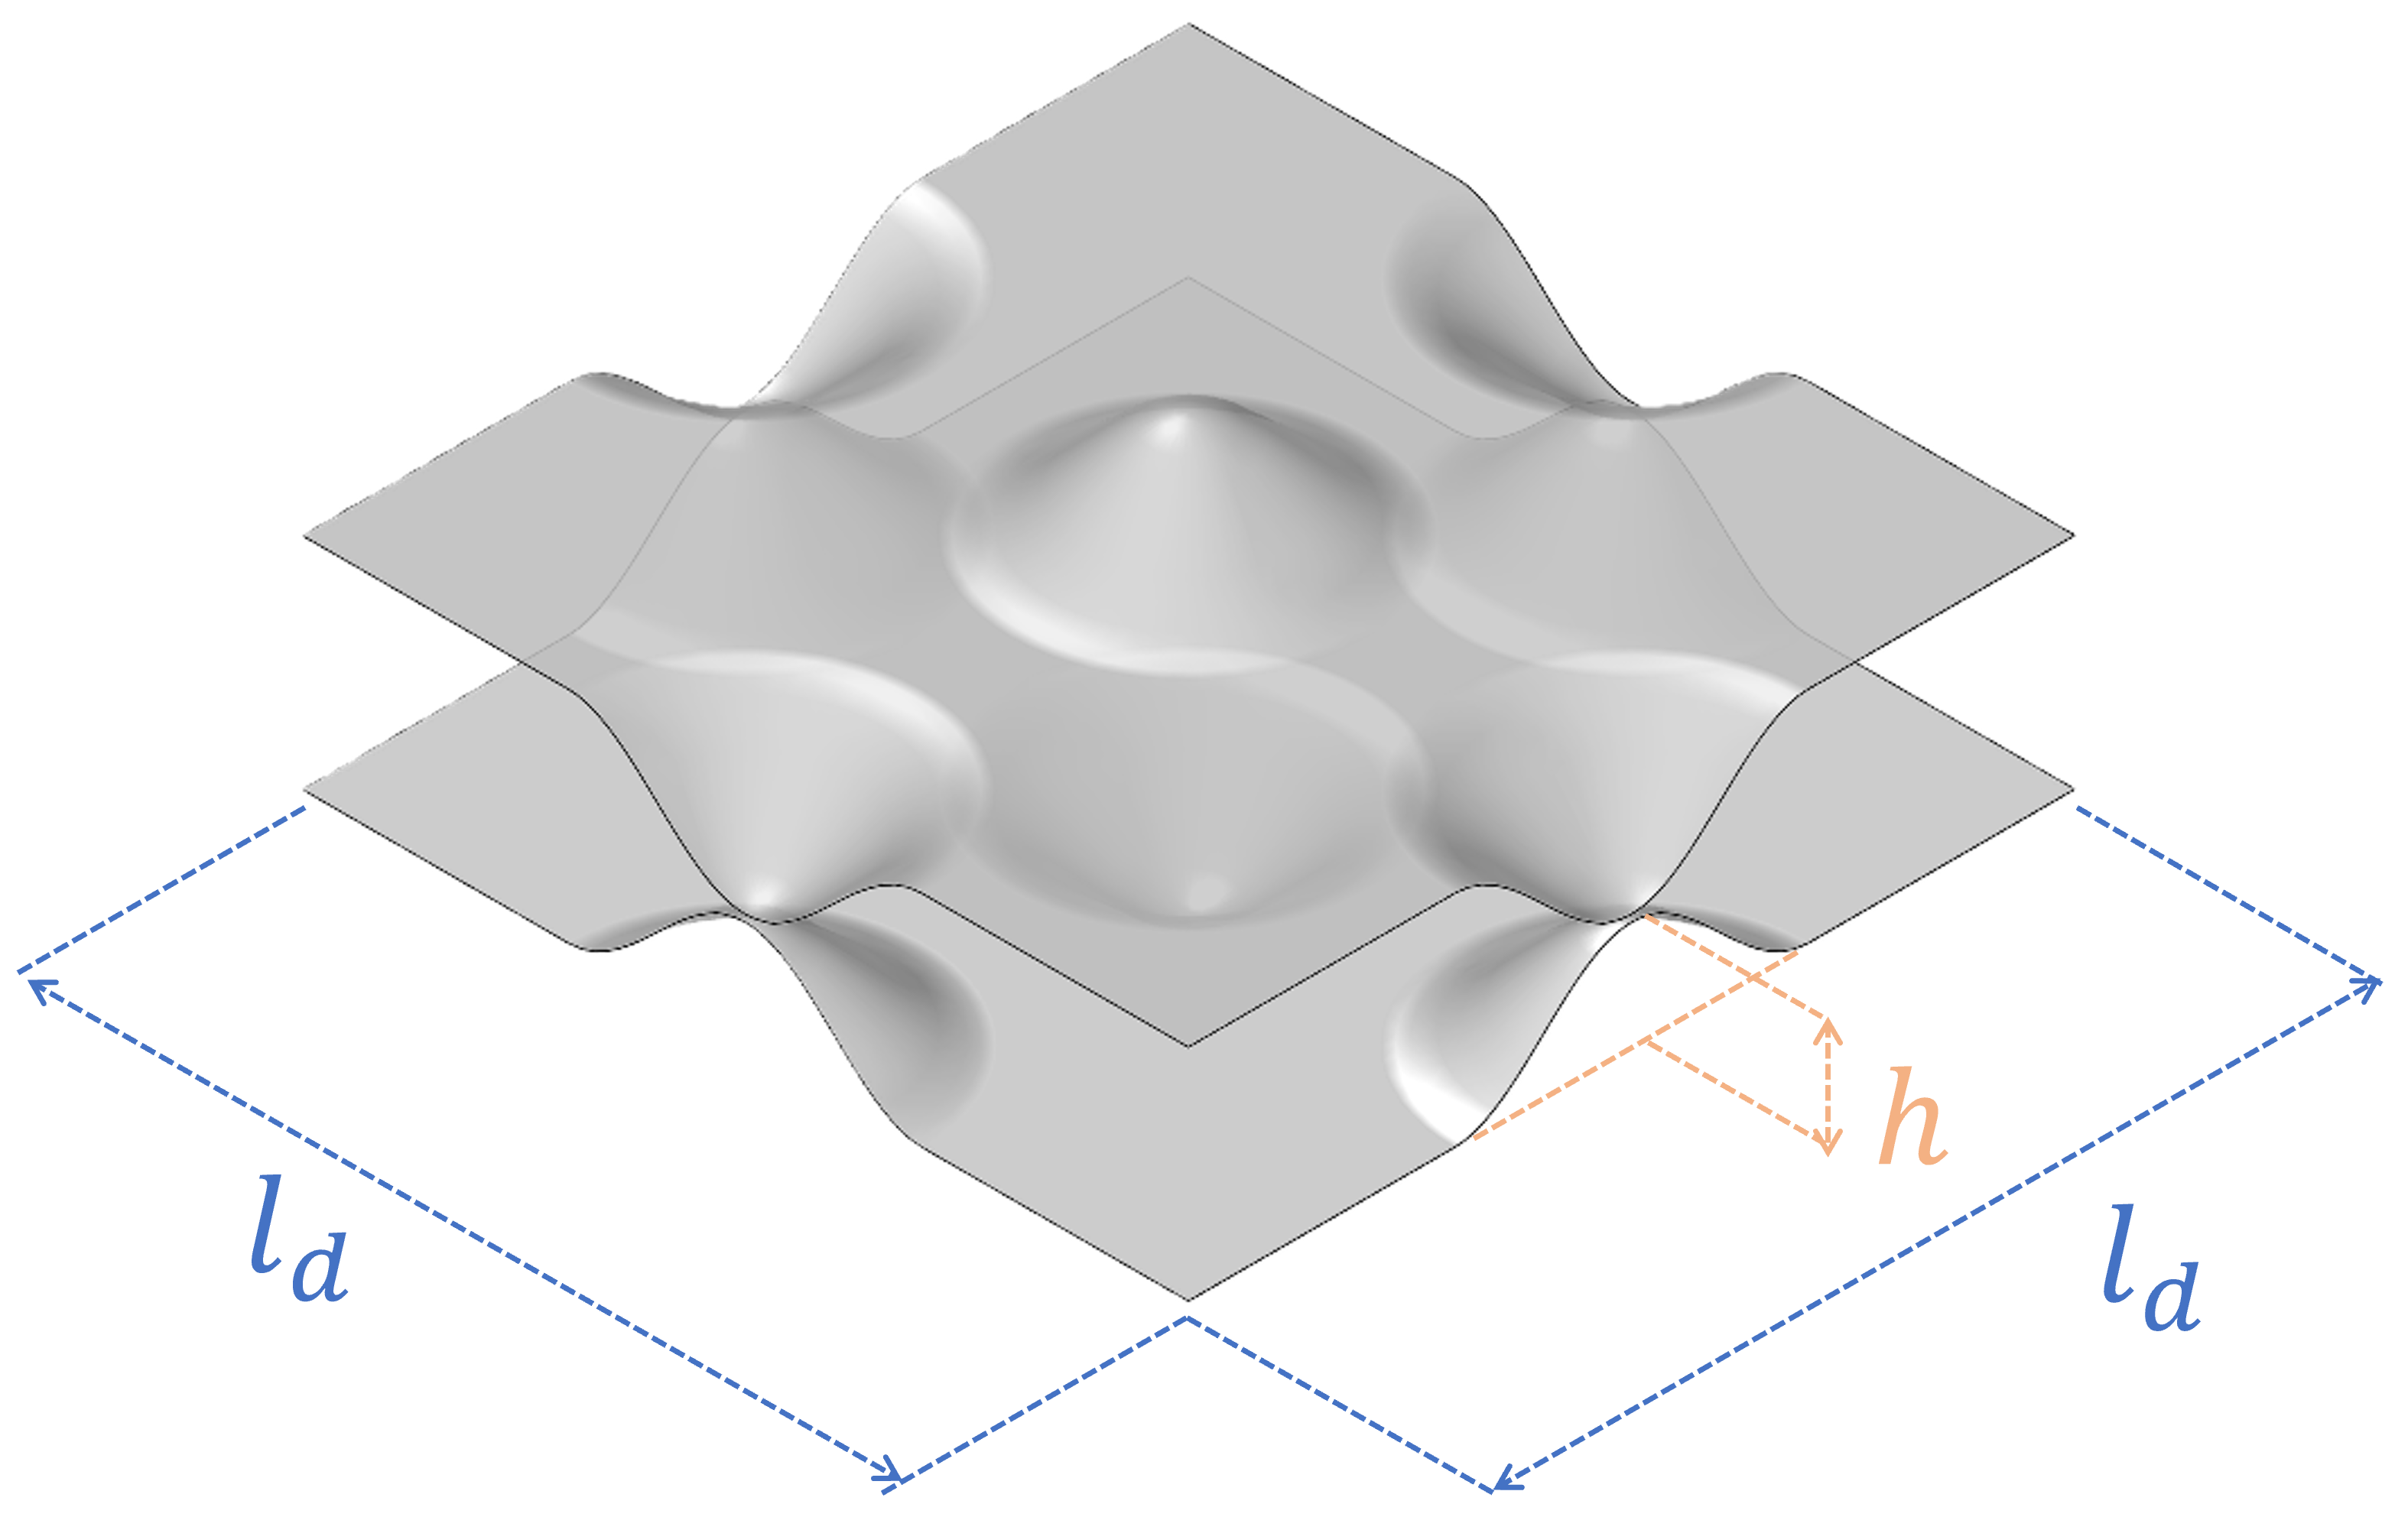
\includegraphics[width=0.3\textwidth]{media/image9_v2.png} &
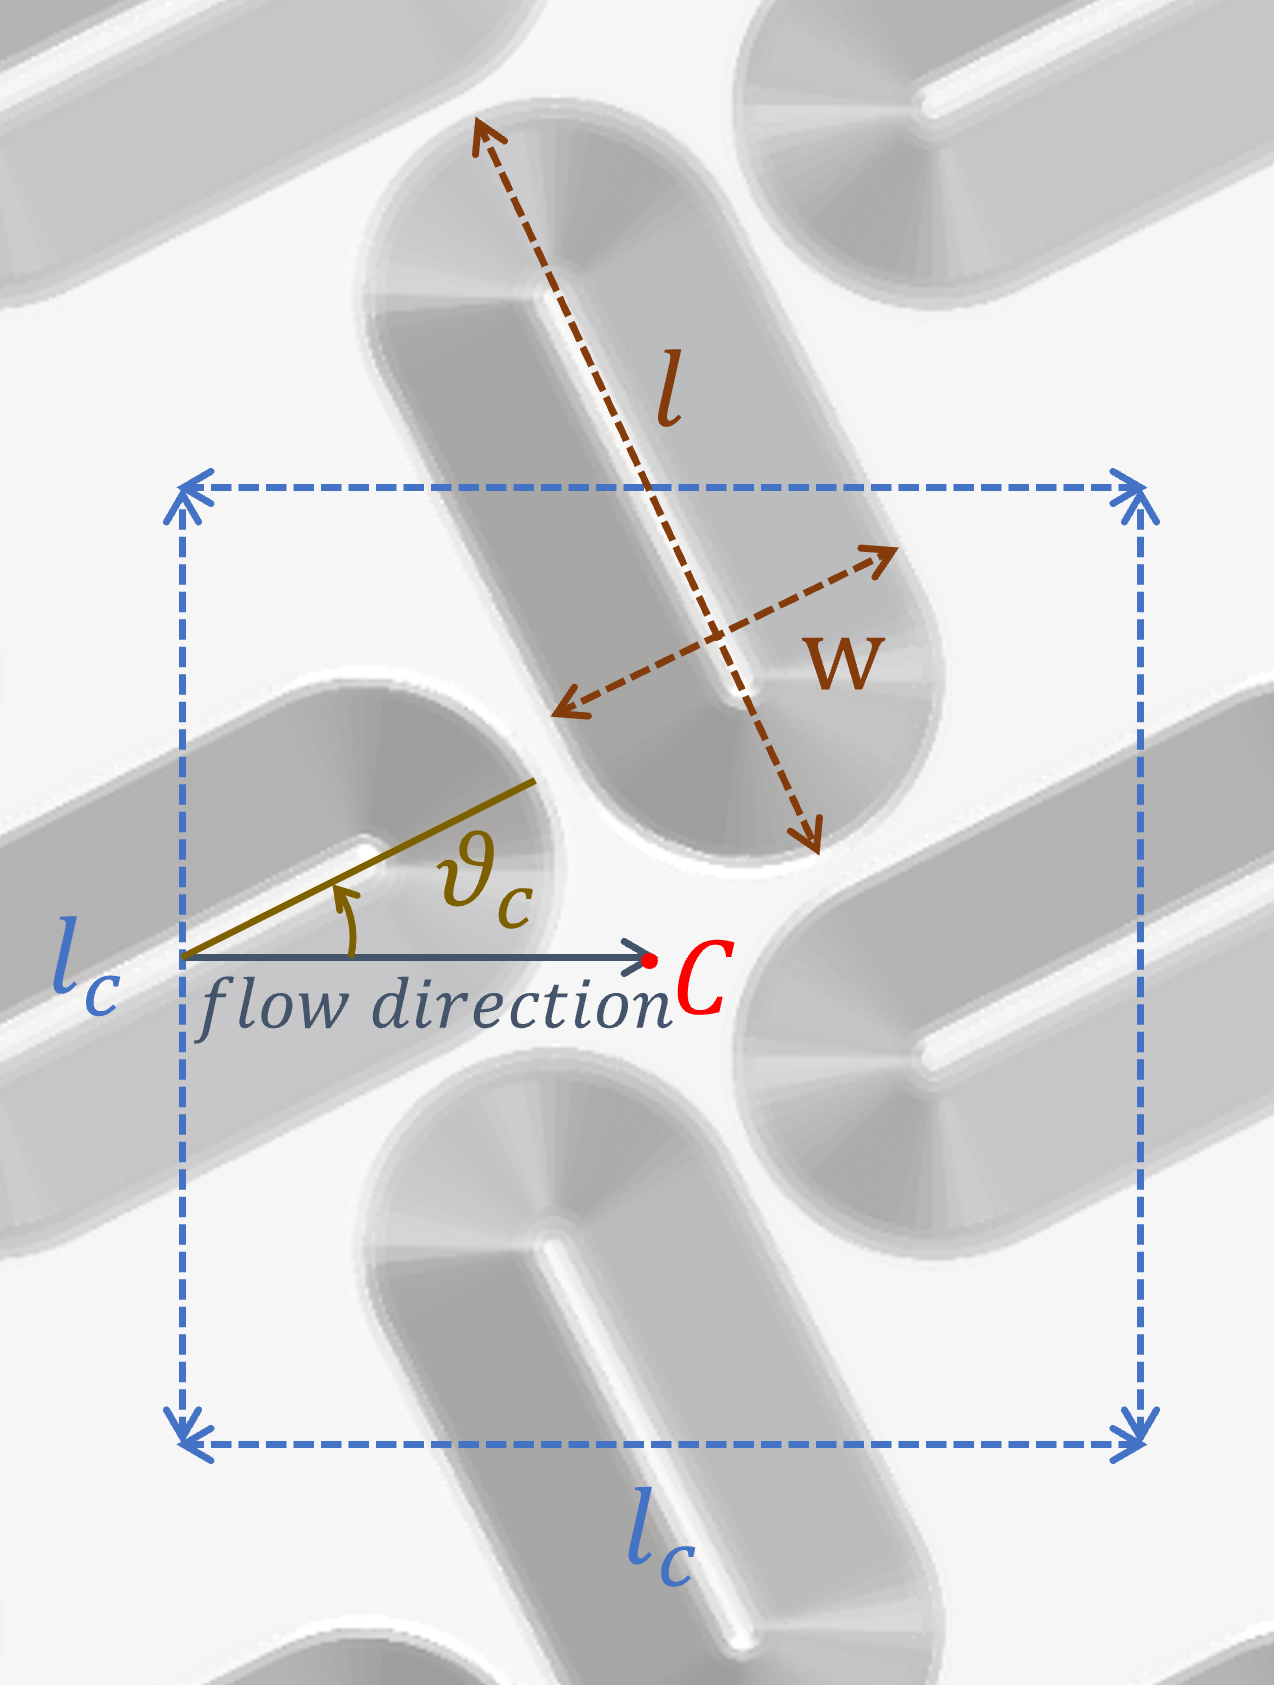
\includegraphics[width=0.2\textwidth]{media/image7_v2.png} &
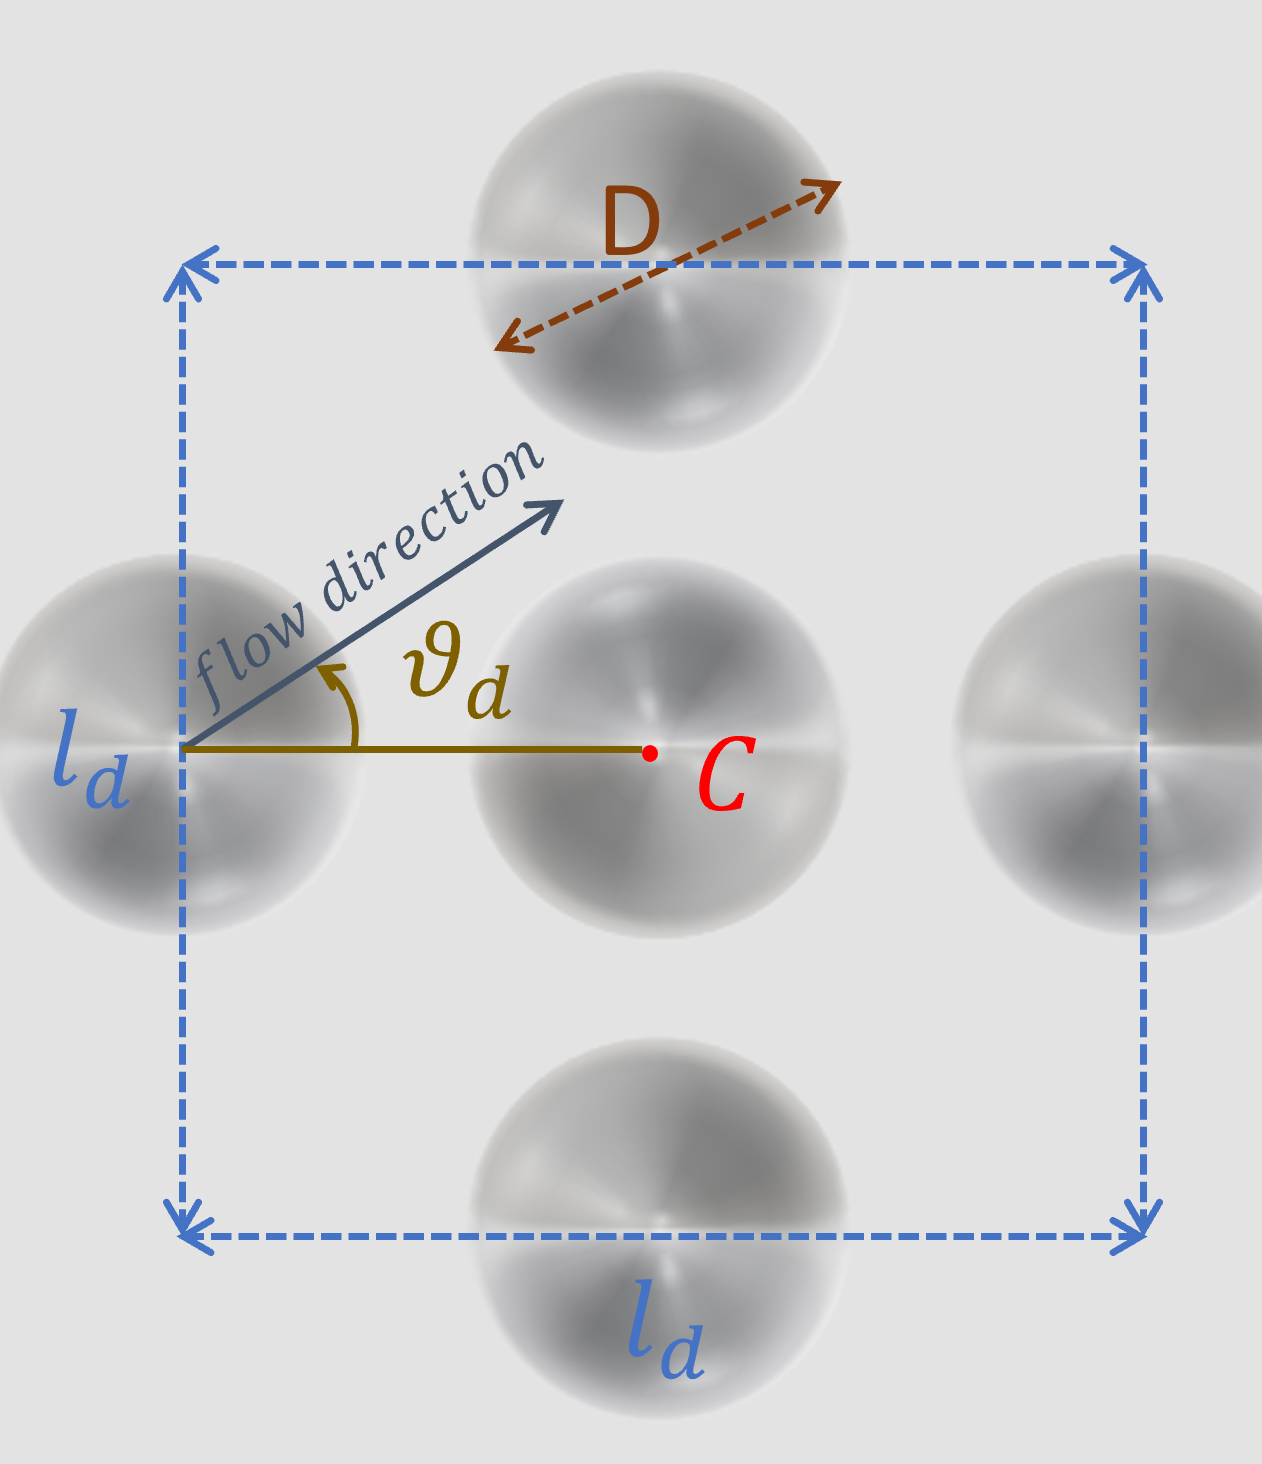
\includegraphics[width=0.2\textwidth]{media/image7.5_v2.png} \\
\end{tabular}
\caption{Unit Cell Dimensions}
\label{figure1}
\end{figure}

\begin{figure}[!ht]
  \centering
    \begin{tabular}{@{}cc@{}}
        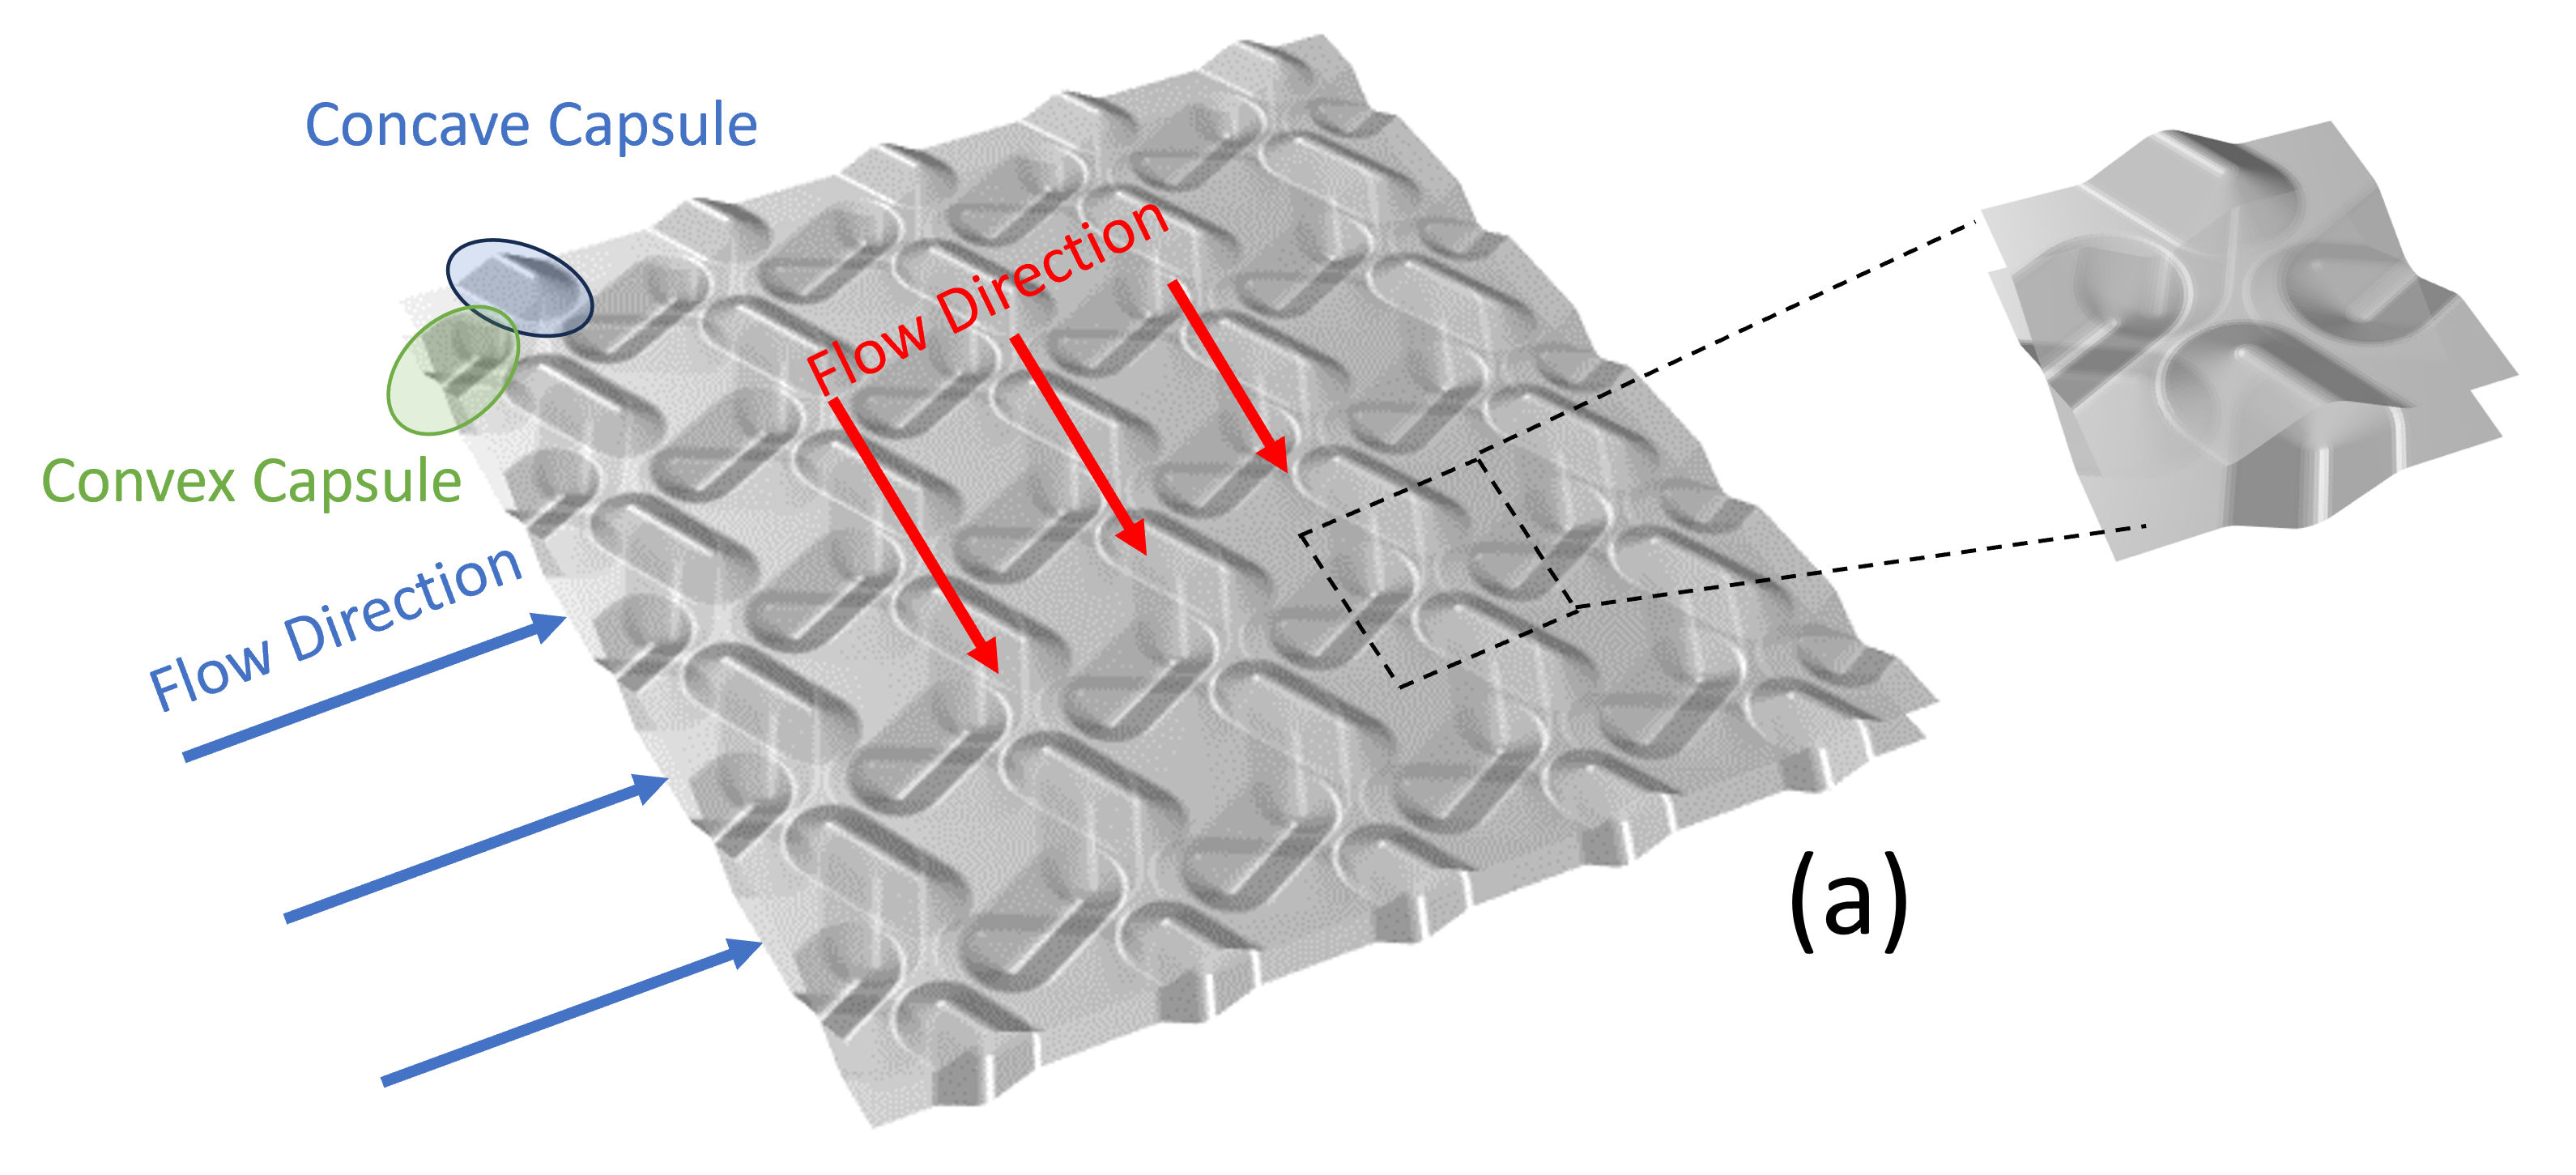
\includegraphics[width=0.5\textwidth]{media/image5_v3.png} &
        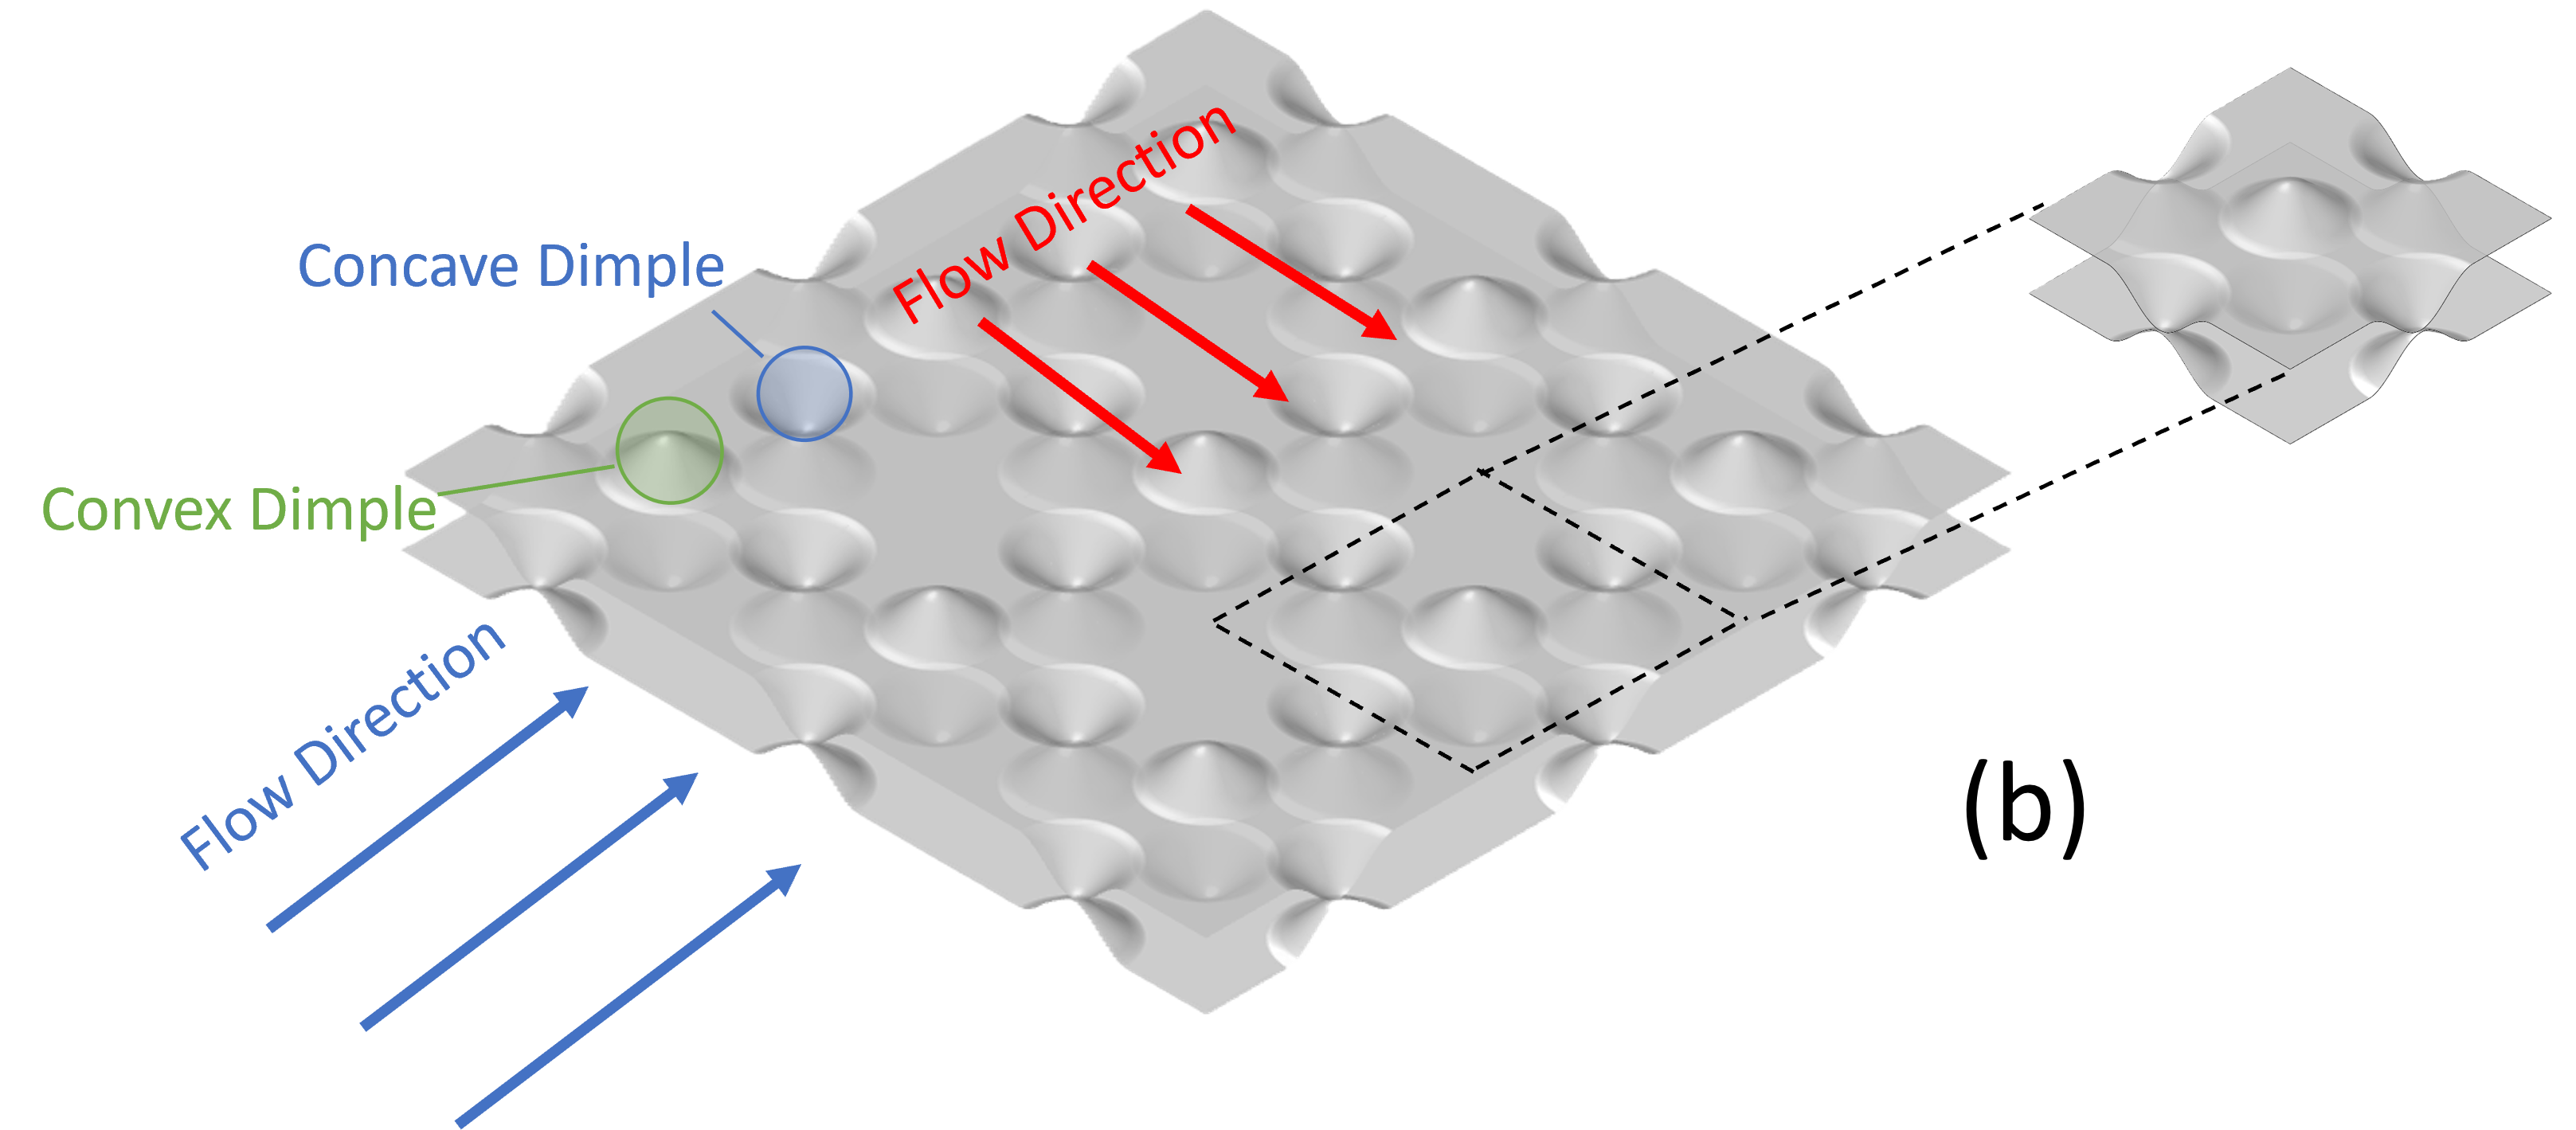
\includegraphics[width=0.5\textwidth]{media/image8_v4.png} \\
    \end{tabular}
  \caption{Schematics and unit cells for (a) a capsule-type plate heat exchanger (CPHE) and (b) a dimple-type plate heat exchanger (DPHE). Blue and green labels identify concave and convex embossings, respectively.}
  \label{figure2}
\end{figure}

\begin{table}[H]
\centering
\caption{Dimensions of the initial geometry}
\label{tab:dim-initial}
\renewcommand{\arraystretch}{1.3}
\begin{tabular}{lcccccc}
\hline
\textbf{Type} & $l$ (mm) & $w$ or $D$ (mm) & $l_c$ or $l_d$ (mm) & $h_c$ or $h_d$(mm) & $\theta_c$ or $\theta_d$ (deg) \\
\hline
CPHE & 20 & 10 & 25 & 2 & 0\degree \\
\hline
DPHE &  & 10 & 25 & 2 & 0\degree \\
\hline
\end{tabular}
\end{table}

\subsubsection{CPHE}
\label{sec:cphe_geometry}

Figure~\ref{figure2} shows the CPHE channel formed between two capsule-embossed plates. Consecutive plates are inverted and rotated, so alternating concave and convex embossings form the spiral-like pattern of two concave and two convex capsules shown in Figure~\ref{figure1}. The geometric parameters are capsule length ($l$), width ($w$), height ($h_c$), unit-cell length ($l_c$), angle ($\theta_c$), and centre $C$, defined by the intersection of perpendicular lines through the capsule midpoints. The angle $\theta_c$ is measured anticlockwise from the mainstream flow direction to the capsule major axis; at $0\degree$, they are aligned. Higher angles rotate the capsule CAD anticlockwise while the flow-entry direction remains fixed normal to the inlet, with $l$, $w$, $h_c$, and $l_c$ unchanged. Table~\ref{tab:dim-initial} lists the initial dimensions.

\subsubsection{DPHE}
\label{sec:dphe_geometry}

Figure~\ref{figure2} shows the DPHE channel and unit cell formed by plates with opposing dimple embossings. The same unit-cell approach is used, with dimple height ($h_d$), diameter ($D$), and unit-cell length ($l_d$) as the main dimensions. Because each dimple is circular, the CAD geometry remains fixed during the angle sweep. The flow-entry angle $\theta_d$ is measured from the fixed line joining adjacent dimple centres to the mainstream flow direction (Figure~\ref{figure1}) and is varied by changing the direction from which flow enters the unchanged dimple array. Table~\ref{tab:dim-initial} lists the initial dimensions.

\subsubsection{Boundary Conditions}
\label{sec:periodic_boundary}

 Periodic boundary condition had been applied on the span-wise direction of the unit cell ($y$-axis). For the stream-wise direction ($x$-axis), a quasi-periodic approach had been implemented. Uniform velocity profile and estimated turbulent parameter setting had been applied for initial simulation. Once the simulation converges it is considered the completion of a quasi-period. The flow parameters from the previous period, such as velocity and kinetic turbulent energy of the outlet boundary, are set as the inlet profile for the next period and the inlet temperature is set as 293~K. When the pressure loss $\Delta p$ and heat transfer coefficient $h_{ave}$ of the last few periods converge, it is considered that the flow and heat transfer are fully developed, and the data will be obtained for analysis \citep{jiang2019,jiang2020,zhang2016}. In addition, the plates are set as a no-slip wall boundary condition with a constant wall temperature of 333~K, and velocity inlet and pressure outlet boundary condition is applied at the inlet and outlet plane respectively.

The same convergence criterion was applied to all 29 cases: a case was deemed converged once the $\Delta p$ and $h_{ave}$ between successive iterations were equal or differed less than 3$\%$. This consistent stopping rule ensures that every reported data point represents a genuinely converged flow state obtained under identical procedural conditions.

\subsubsection{Geometric parameters}
\label{sec:geometric_parameters}

A one-factor-at-a-time analysis is used to isolate the effects of capsule angle, capsule height, dimple height, and dimple flow-entry angle. Table~\ref{tab:geom_cases} summarizes the four seven-case sweeps, the fixed variables in each sweep, and the targeted combined dimple case. The tested ranges follow prior studies and commercially available products \citep{hamedi2024, jiang2019, jiang2019a, jiang2020, soman2019, mocnik2024, jing2019, Alfalaval2022}. All cases use the same numerical setup. The recorded thermo-fluid outputs include Nu, $f$, $\Delta p$, and turbulence kinetic energy fields.

After the one-factor sweeps, one interaction case combines $\theta_d=45\degree$ with $h_d=5.0$~mm. It is reported separately from the two seven-case dimple sweeps.

\subsubsection{Performance evaluation criteria}
\label{sec:performance_criteria}

The following performance metrics are used to compare the results:

\begin{itemize}
  \item \textbf{Nusselt Number} (Nu): Measures convective heat transfer relative to conduction across the fluid layer. Higher Nu indicates stronger convective heat transfer.

  \item \textbf{Friction Factor} ($f$): Measures flow resistance from the simulated pressure loss, as defined by Equation~\eqref{eq:f}.

  \item \textbf{Performance Evaluation Criterion} (PEC): Combines heat transfer and flow resistance to rank all 29 cases on a common scale:
  \begin{equation}
  \text{PEC} = \frac{\text{Nu}}{f^{1/3}}
  \label{eq:PEC}
  \end{equation}
  Higher PEC indicates a better heat-transfer--friction trade-off under the common comparison basis used here. PEC is widely used to compare the thermal--hydraulic performance of plate heat exchangers \citep{hamedi2024,jiang2019,jiang2020, kumar2019, piper2019, shao2024, zhang2016}.
  Sections~\ref{sec:disc_capsule_angle}--\ref{sec:disc_dimple_angle} analyze trends in Nu and $f$ individually; section~\ref{sec:tgg_comparison} uses PEC to rank all cases and compare both embossing families.
\end{itemize}

The comparison identifies heat-transfer and flow-resistance trade-offs among the examined cases. Because each primary sweep changes one geometric variable while the others remain fixed and only one targeted combined case is included, the results do not establish a global optimum across interacting variables or untested conditions.

\paragraph{Relative Embossing Depth (RED)}
Embossing depth constrains plate spacing and channel size. Relative Embossing Depth (RED) is introduced to compare the protrusion height with the effective channel scale:
\begin{equation}
\text{RED} = \frac{h}{D_e}
\label{eq:red}
\end{equation}
where $h$ is the embossing height of the feature ($h_c$ for capsule cases, $h_d$ for dimple cases) and $D_e$ is the hydraulic diameter of the corresponding channel (Equation~\eqref{eq:De}). For "capsule-angle" cases, $D_e$ changes slightly with angle because of the capsule geometry, and therefore the inlet area $A_0$ varies with $\theta_c$. For "dimple-angle" cases, the flow angle is the only variable thus RED would remain constant. RED captures the fact that every geometric modification ultimately alters the ratio of embossing protrusion to effective channel size, regardless of whether the varied parameter is an angle or a height.

It should be noted that RED is a derived quantity: recovering the specific geometric case from a given RED value requires knowledge of the corresponding $D_e$, which in turn depends on the full unit-cell geometry (Equation~\eqref{eq:De}). However, because each parametric family varies only one geometric variable at a time, the mapping from RED back to the physical parameter is unambiguous within each family.

\begin{table}[H]
\centering
\caption{Geometric parameter cases for CPHE and DPHE}
\label{tab:geom_cases}
\footnotesize
\renewcommand{\arraystretch}{1}
\begin{tabularx}{\textwidth}{ll>{\raggedright\arraybackslash}l>{\raggedright\arraybackslash}X}
\hline
\textbf{Heat Exchanger Type} & \textbf{Parameter} & \textbf{Cases} & \textbf{Description} \\ \hline
\multirow{2}{*}{CPHE (Capsule-Type)} 
& Capsule Angle ($\theta_c$) & 0\degree\ to 45\degree & Orientation of capsule pattern relative to main flow direction with 7.5\degree\ increments and a capsule height of 2.5~mm. \\
& Capsule Height ($h_c$) & 2--5~mm & Height of capsule embossing feature with 0.5~mm increments and a capsule angle of 22.5\degree. \\ \hline
\multirow{3}{*}{DPHE (Dimple-Type)} 
& Dimple Height ($h_d$) & 2--5~mm & Height of the dimple embossing feature with 0.5~mm increments and a dimple angle of 0\degree. \\
& Dimple Angle ($\theta_d$) & 0\degree\ to 45\degree & Angle between the main flow direction and the dimple pattern, varied in 7.5\degree\ increments with a dimple height of 3.5~mm. \\
& Combined Dimple Case & $\theta_d=45\degree$, $h_d=5.0$~mm & Targeted interaction case combining the highest-PEC dimple orientation with the maximum tested dimple height. \\ \hline
\end{tabularx}
\end{table}

\subsection{Mesh independence}
\label{sec:mesh}

An unstructured poly-hexacore mesh type is adopted for the mesh generation. With guidance from literature, certain criteria are set for the mesh generated to minimize discretizations and interpolation error \citep{sorgente2023, juretic2010}, including mesh orthogonality and mesh skewness. For this study, the criteria of minimum mesh orthogonality of 0.1 and maximum mesh skewness of 0.8 are set for all cases.

To accurately predict the wall heat transfer coefficient and the wall shear stress close to the wall, prism layers are included in the mesh generation. Prism layers are hexahedral cells that are normal to the wall boundary to capture the steep normal gradient in the mean velocity and temperature inside the thermal and hydraulic boundary layers. The total prism layer thickness should capture the turbulent boundary layer of the flow. The initial estimation of the total boundary layer thickness $\delta$ can be estimated through the following equation: $\delta/x = 0.16/\text{Re}_x^{1/7}$ \citep{cengel2014}, where $x$ is the total stream length, which is $l_c$ and $l_d$ for this study, and Re is the Reynolds number.

For the prism layers to accurately predict the near-wall behavior, the first prism layer thickness (or the first layer height) plays an important role in calculating the behavior at the viscous sub-layer, as it is related to $y^+$, which is a dimensionless distance normal to the wall, and the near-wall kinematic viscosity can be calculated accordingly. As suggested by \citet{eca2018}, to minimize the numerical uncertainty, $y^+$ ~0.1 should be applied for the SST $k$--$\omega$ turbulence model; therefore, the first layer height is set to 0.0002~mm, with 7 boundary layers and transition ratio as 0.5, the resultant $y^+$ is 0.087 (Figure~\ref{figure3}).

A mesh independence study is performed for CPHE with $h = 2.5$~mm, as shown in Figure~\ref{figure3}. $f$ and Nu for five different meshes ranging from $\sim$100k to $\sim$1.1M elements are compared to determine the best coarsest mesh. The difference of $f$ and Nu between the results of $\sim$800k mesh count and $\sim$1.1M mesh count is less than 2.7\% and 2\%, respectively, showing the results obtained from $\sim$800k mesh count are reliable and validated, and will be employed in this study.

\begin{figure}[!ht]
  \centering
\begin{tabular}{cc}
        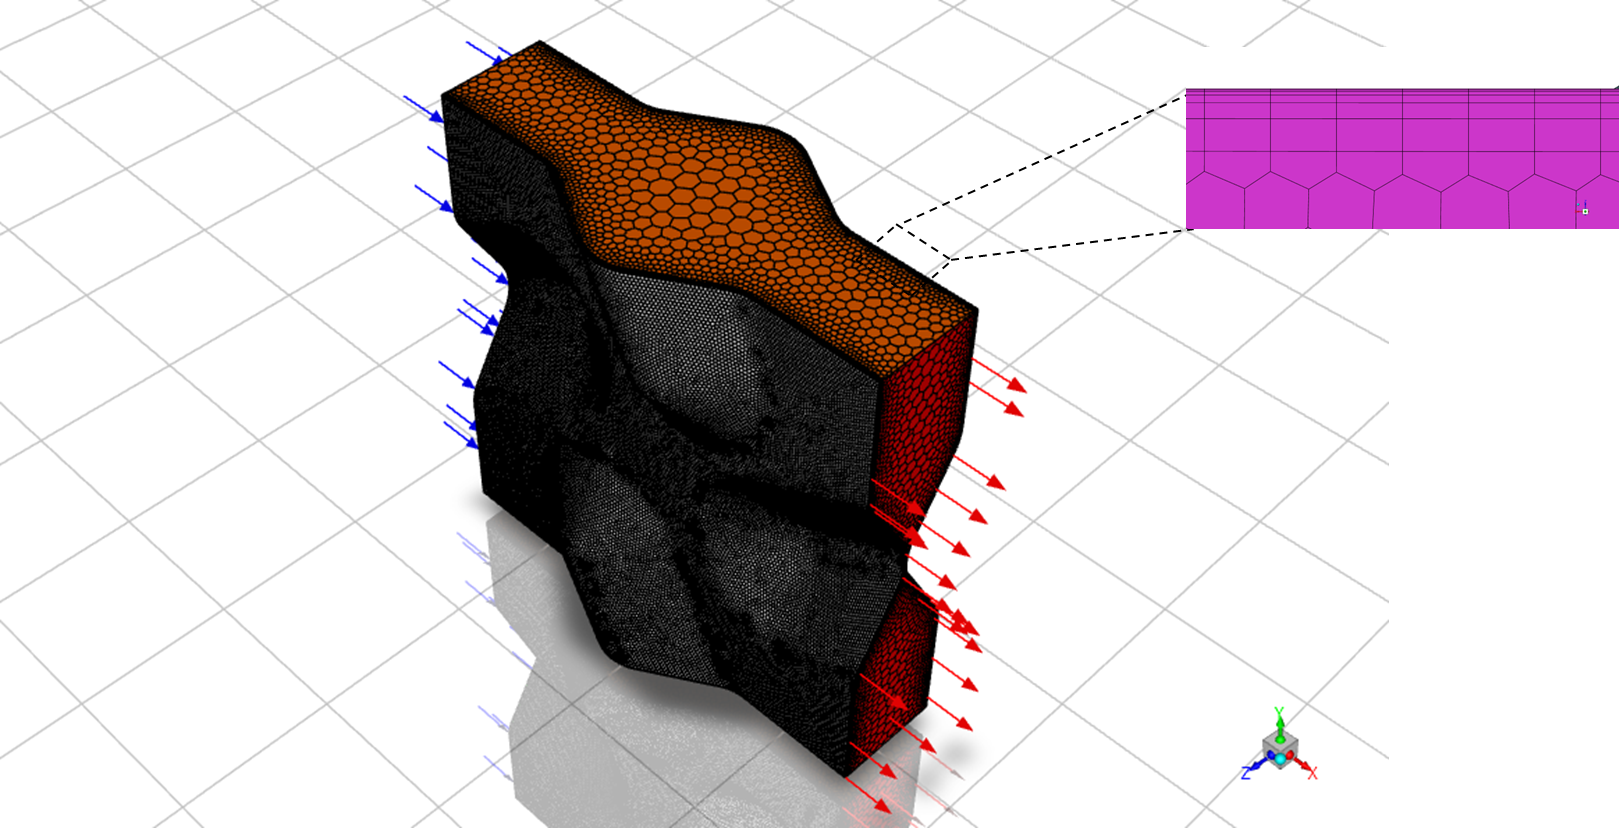
\includegraphics[width=0.5\textwidth]{media/Picture4.png} &
        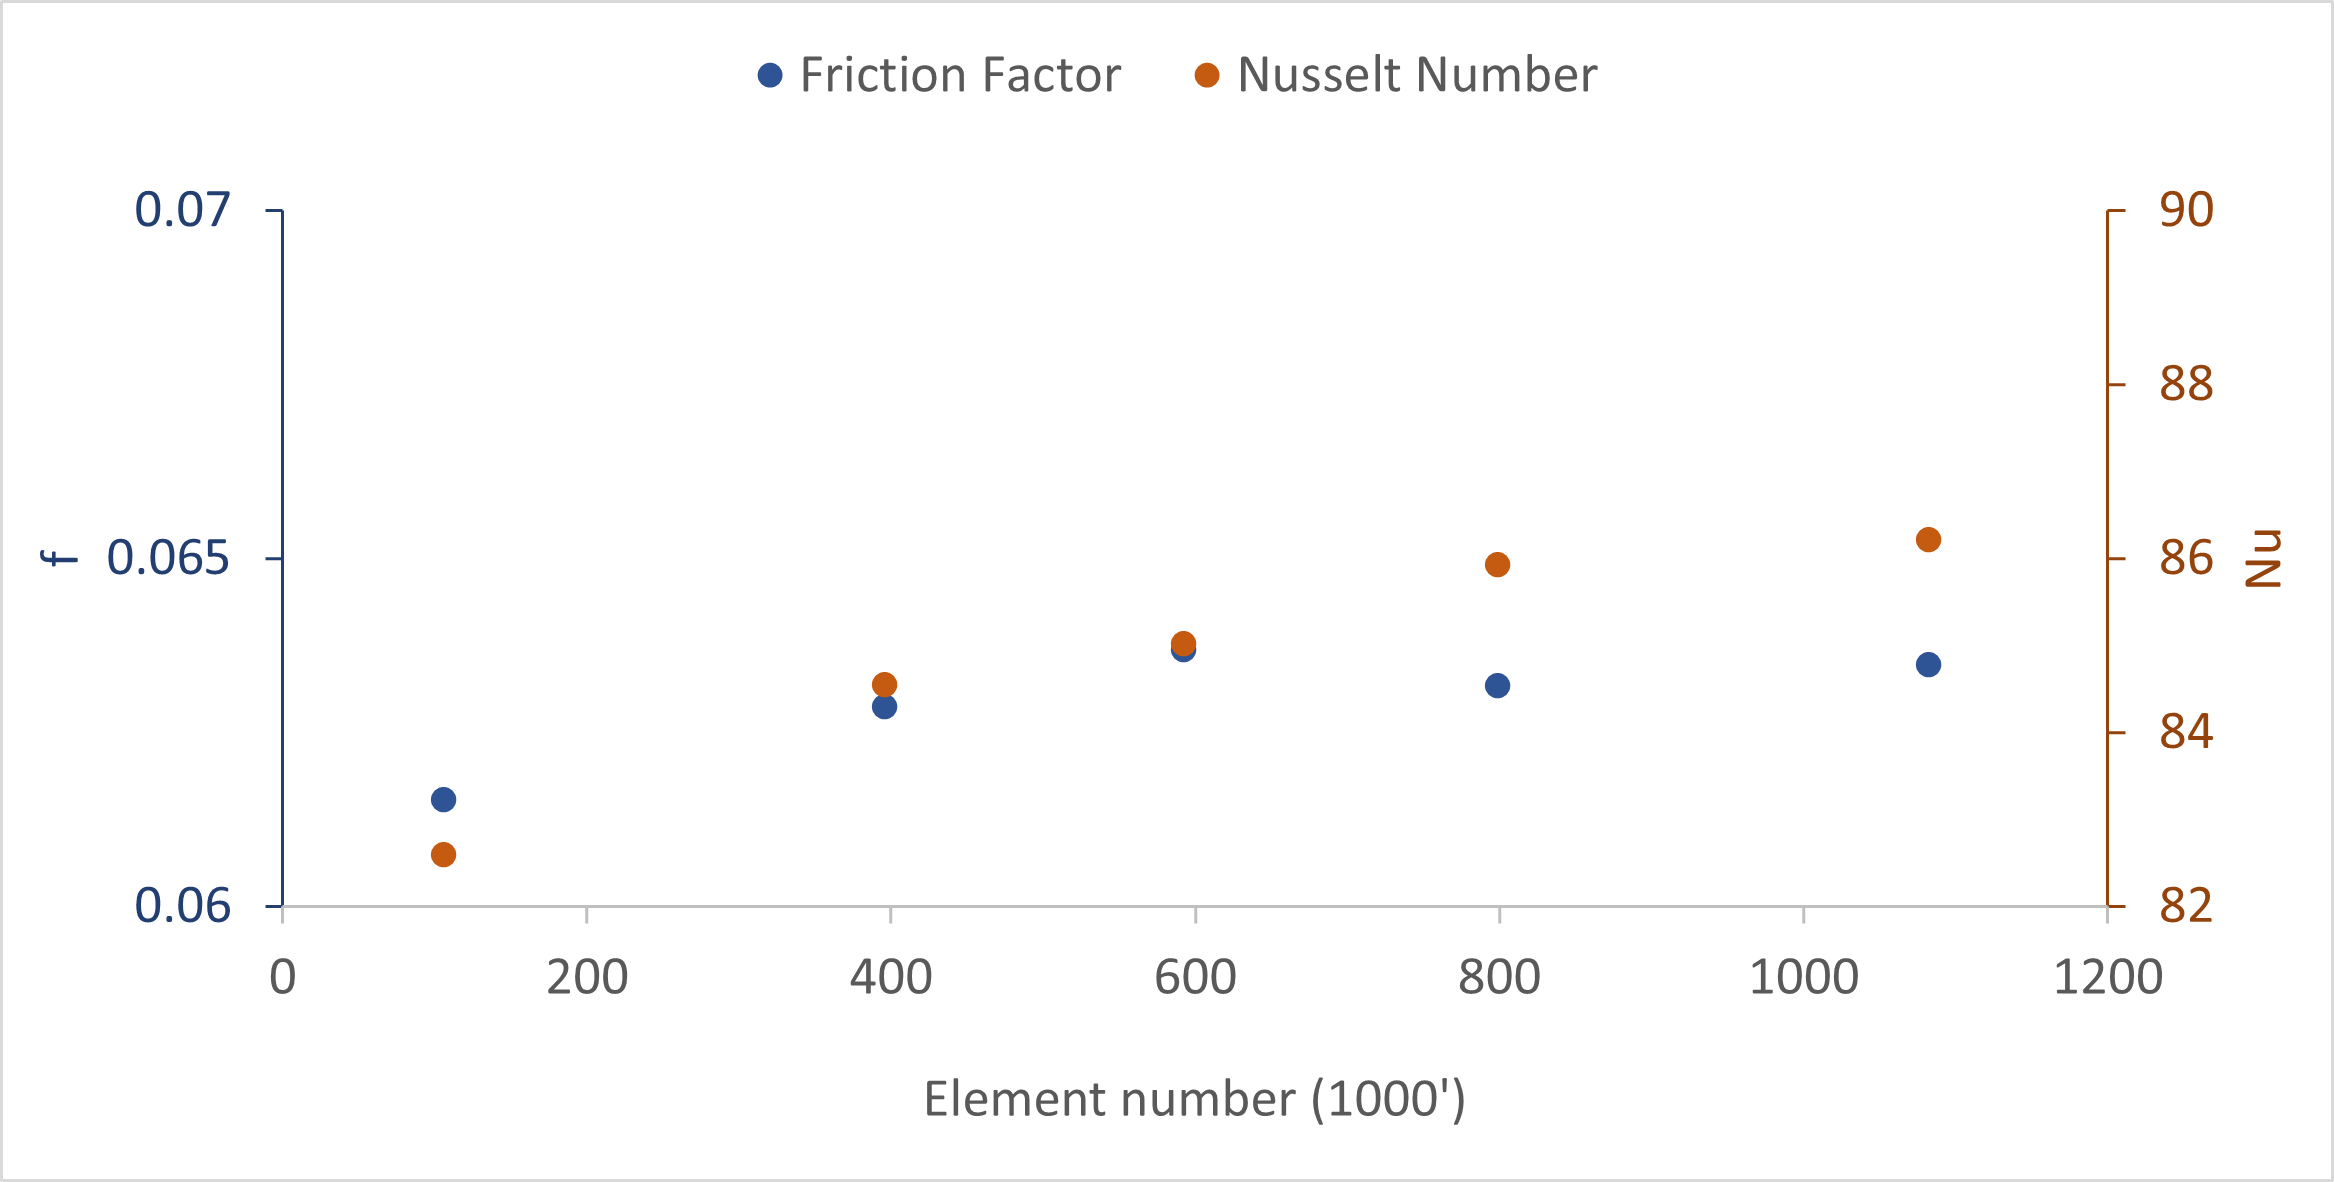
\includegraphics[width=0.5\textwidth]{media/image10_v1.png} \\        
    \end{tabular}
  \caption{Mesh Independence Study}
  \label{figure3}
\end{figure}


\section{Results and Discussion}
\label{sec:results}
\label{sec:discussion}

The numerical simulations conducted in this study provide detailed insight into the thermo-hydraulic behavior of capsule-type and dimple-type plate heat exchangers under a variety of geometric configurations. By examining the influence of selected design parameters namely the capsule angle and height in CPHE, and the dimple height and angle of flow in DPHE the impact on flow structures, pressure drop, and heat transfer performance is assessed. Key fluid dynamic behaviors, including vortex generation, turbulence intensity, and recirculating flow patterns, are visualized through turbulence kinetic energy contours and streamline plots. Temperature distributions further reveal the relationship between geometric enhancements and thermal mixing. These findings enable the identification of design trends that balance improved heat transfer effectiveness with manageable pressure penalties, supporting the development of more efficient compact heat exchanger designs. Figure~\ref{figure4} provides an overview of the four parametric sweeps by comparing the friction factor and Nusselt number for capsule angle, capsule height, dimple height, and dimple angle. The following subsections relate these performance trends to the corresponding flow and temperature fields.

% Figure 4: merged Nu--f comparisons for the angle and height sweeps.
% The two source plots remain separate so the panel layout stays editable in LaTeX.
\begin{figure}[H]
    \centering
    \begingroup
    \newlength{\figfourpanelwidth}
    \setlength{\figfourpanelwidth}{0.485\linewidth}

    \newcommand{\figfourpanel}[3]{%
        \begin{tabular}[t]{@{}c@{}}
            \includegraphics[width=\figfourpanelwidth]{#1}\\[-1pt]
            {\sffamily\bfseries\fontsize{8.5}{9.5}\selectfont (#2) #3}
        \end{tabular}%
    }

    \begin{tabular}[c]{@{}c@{\hspace{0.02\linewidth}}c@{}}
        \figfourpanel{media/Figure4_angle_comparison.png}{a}{Angle sweeps, $\theta_c$ and $\theta_d$} &
        \figfourpanel{media/Figure4_height_comparison.png}{b}{Height sweeps, $h_c/l_c$ and $h_d/l_d$}
    \end{tabular}
    \endgroup
    \caption{Fanning friction factor $f_F$ (blue) and two-wall Nusselt number Nu (orange), referenced to each case's fluid-domain mass-average temperature, for the four parametric sweeps: (a) capsule-angle and dimple-angle sweeps and (b) normalized capsule-height and dimple-height sweeps. The combined dimple case is excluded from these one-factor sweeps and is shown separately in Figure~\ref{figure15}.}
    \label{figure4}
\end{figure}


\subsection{CPHE parametric study}
\label{sec:cphe_results}

Two major improvements or modifications are proposed in this study to investigate the impact on the pressure drop and heat transfer rate: 1) the angle between the capsule and the mainstream; 2) the capsule height.

\subsubsection{Capsule angle}
\label{sec:disc_capsule_angle}

For the capsule-angle sweep defined in Table~\ref{tab:geom_cases}, Figures~\ref{figure5} and~\ref{figure6} show representative mid-plane TKE fields and two-dimensional streamlines at $\theta_c=0\degree$, $22.5\degree$, and $45\degree$, while Figure~\ref{figure4}(a) reports the friction factor and Nusselt number for all seven cases.

At $\theta_c=0\degree$, Figure~\ref{figure5}(a) shows streamwise high-TKE bands on either side of a low-TKE central wake. Rotating the capsules to $22.5\degree$ breaks this aligned structure: the low-TKE region becomes asymmetric and the highest TKE is concentrated where the redirected wake meets the through-flow (Figure~\ref{figure5}(b)). At $45\degree$, high TKE extends across a larger part of the outer shear regions, while a broad sheltered wake remains behind the capsules (Figure~\ref{figure5}(c)). The angle sweep therefore redistributes the energetic shear regions rather than changing TKE uniformly across the section.

Figure~\ref{figure6} shows the associated streamline topology. At $0\degree$, the wakes and recirculation cells remain aligned with the streamwise passages (Figure~\ref{figure6}(a)). At $22.5\degree$, the through-flow is deflected across the channel and interacts with compact recirculation cells (Figure~\ref{figure6}(b)). At $45\degree$, larger separated and reattaching regions occupy the passage and the secondary flow is distributed more widely (Figure~\ref{figure6}(c)). These changes increase both wall-to-core transport and hydraulic resistance.

% Figure 5: editable LaTeX layout.
% \figfivepanelwidth is the final size; no outer scaling is applied.
\begin{figure}[!ht]
    \centering
    \begingroup
    \newlength{\figfivepanelwidth}
    \newlength{\figfivelegendunit}
    \setlength{\figfivepanelwidth}{1.55in}
    \setlength{\figfivelegendunit}{\dimexpr\figfivepanelwidth*10/52\relax}

  
    \definecolor{figfiveTKE0}{RGB}{4,41,91}
    \definecolor{figfiveTKE1}{RGB}{27,59,111}
    \definecolor{figfiveTKE2}{RGB}{64,76,108}
    \definecolor{figfiveTKE3}{RGB}{89,95,109}
    \definecolor{figfiveTKE4}{RGB}{111,113,115}
    \definecolor{figfiveTKE5}{RGB}{134,131,120}
    \definecolor{figfiveTKE6}{RGB}{159,150,116}
    \definecolor{figfiveTKE7}{RGB}{184,171,108}
    \definecolor{figfiveTKE8}{RGB}{212,193,92}
    \definecolor{figfiveTKE9}{RGB}{239,217,69}

    \newcommand{\figfivelegendbar}{%
        \begin{tikzpicture}[baseline=0pt,x=1cm,y=\figfivelegendunit]
            \fill[figfiveTKE0] (0,0.00) rectangle (0.42,0.52);
            \fill[figfiveTKE1] (0,0.52) rectangle (0.42,1.04);
            \fill[figfiveTKE2] (0,1.04) rectangle (0.42,1.56);
            \fill[figfiveTKE3] (0,1.56) rectangle (0.42,2.08);
            \fill[figfiveTKE4] (0,2.08) rectangle (0.42,2.60);
            \fill[figfiveTKE5] (0,2.60) rectangle (0.42,3.12);
            \fill[figfiveTKE6] (0,3.12) rectangle (0.42,3.64);
            \fill[figfiveTKE7] (0,3.64) rectangle (0.42,4.16);
            \fill[figfiveTKE8] (0,4.16) rectangle (0.42,4.68);
            \fill[figfiveTKE9] (0,4.68) rectangle (0.42,5.20);
            \draw[line width=0.35pt] (0,0) rectangle (0.42,5.20);
            \foreach \y/\ticklabel in {
                0.00/0.0,0.52/1.0,1.04/2.0,1.56/3.0,2.08/4.0,
                2.60/5.0,3.12/6.0,3.64/7.0,4.16/8.0,4.68/9.0,5.20/10.0}
                {\draw[line width=0.3pt] (0.42,\y) -- (0.49,\y)
                 node[anchor=west,font=\sffamily\fontsize{7.5}{8}\selectfont]
                 {\ticklabel};}
        \end{tikzpicture}%
    }

    \newcommand{\figfivepanellabel}[2]{%
        {\sffamily\bfseries\fontsize{8.5}{9.5}\selectfont
         (#1) $\theta_c=#2^{\circ}$}%
    }

    \begin{tabular}[c]{@{}l@{\hspace{0.10in}}c@{\hspace{0.05in}}c@{\hspace{0.05in}}c@{}}
        {\sffamily\bfseries\fontsize{8.5}{9.5}\selectfont
         \shortstack[l]{Turbulence kinetic\\energy, $k$}} & & & \\[-1pt]
        \figfivelegendbar &
        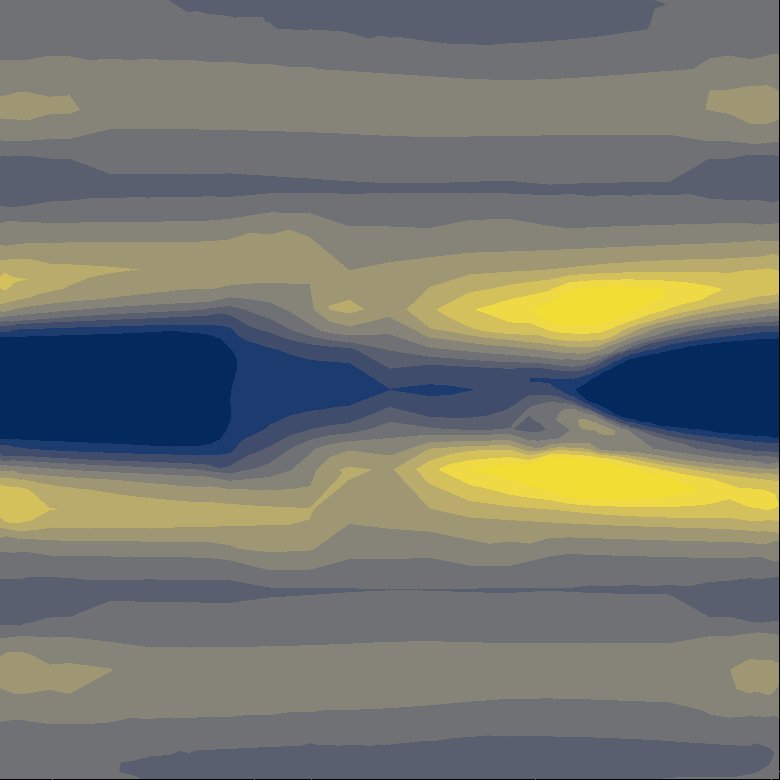
\includegraphics[width=\figfivepanelwidth]{image_2/Figure6/CA_0deg_TKE.png} &
        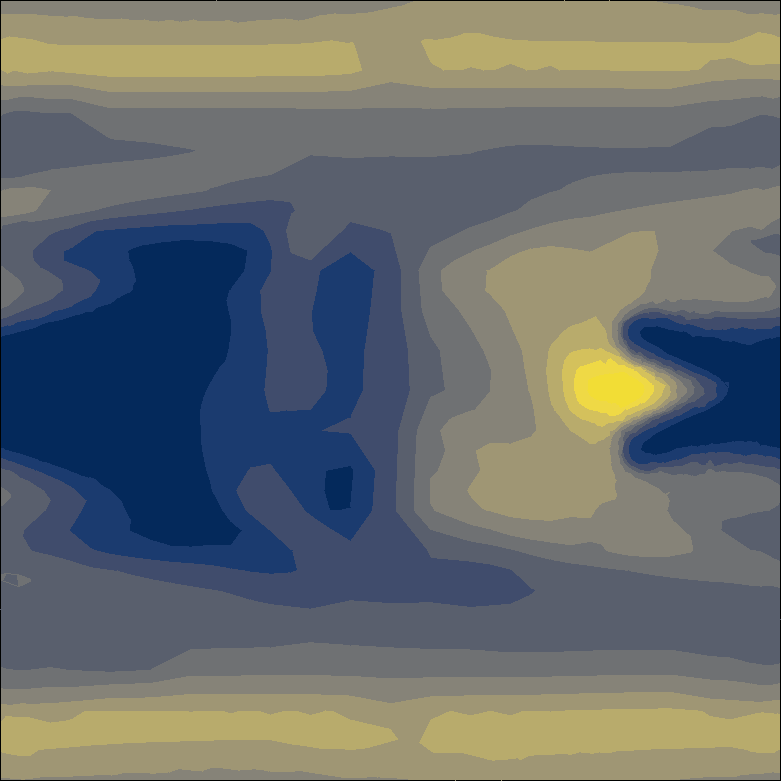
\includegraphics[width=\figfivepanelwidth]{image_2/Figure6/CA_22.5deg_TKE.png} &
        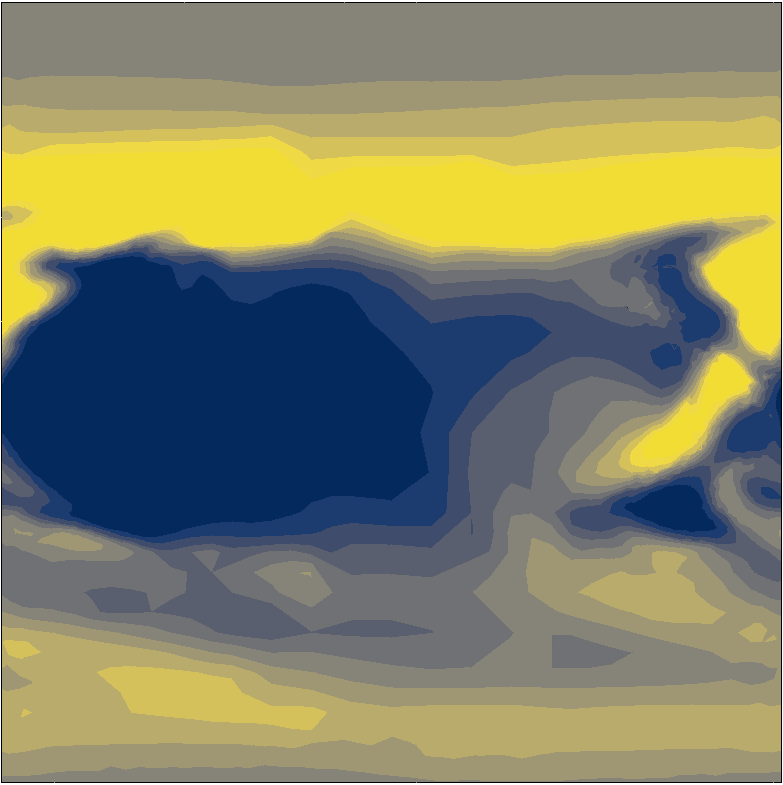
\includegraphics[width=\figfivepanelwidth]{image_2/Figure6/CA_45deg_TKE.png} \\[-1pt]
        {\sffamily\fontsize{7.5}{8.5}\selectfont
         \shortstack[l]{$\times 10^{-3}$\\$\mathrm{m^2\,s^{-2}}$}} &
        \figfivepanellabel{a}{0} &
        \figfivepanellabel{b}{22.5} &
        \figfivepanellabel{c}{45}
    \end{tabular}
    \endgroup
    \caption{TKE distribution of the middle $z$-axis section of CPHE at representative capsule angles ($\theta_c=0\degree$, $22.5\degree$, and $45\degree$).}
    \label{figure5}
\end{figure}


% Figure 6: editable LaTeX layout.
% Change \figuresixpanelwidth or the tabular spacing below to adjust the layout.
\begin{figure}[!ht]
    \centering
    \begingroup
    \newlength{\figuresixpanelwidth}
    \setlength{\figuresixpanelwidth}{0.31\textwidth}

    \tikzset{
        figuresixcallout/.style={
            fill=white,
            fill opacity=0.86,
            text opacity=1,
            rounded corners=0.8pt,
            inner sep=1.2pt,
            align=center,
            font=\sffamily\bfseries\fontsize{5.8}{6.3}\selectfont
        },
        figuresixarrow/.style={
            ->,
            >=stealth,
            draw=black!70,
            line width=0.45pt
        }
    }

    \newcommand{\figuresixlabel}[2]{%
        {\sffamily\bfseries\fontsize{8.5}{9.5}\selectfont
         (#1) $\theta_c=#2^{\circ}$}%
    }

    \newcommand{\figuresixpanel}[3]{%
        \begin{tabular}[t]{@{}c@{}}
            \includegraphics[width=\figuresixpanelwidth]{#1}\\[-1pt]
            \figuresixlabel{#2}{#3}
        \end{tabular}%
    }

    \newcommand{\figuresixpanela}{%
        \begin{tabular}[t]{@{}c@{}}
            \begin{tikzpicture}
                \node[anchor=south west,inner sep=0] (figuresixaimage) at (0,0)
                    {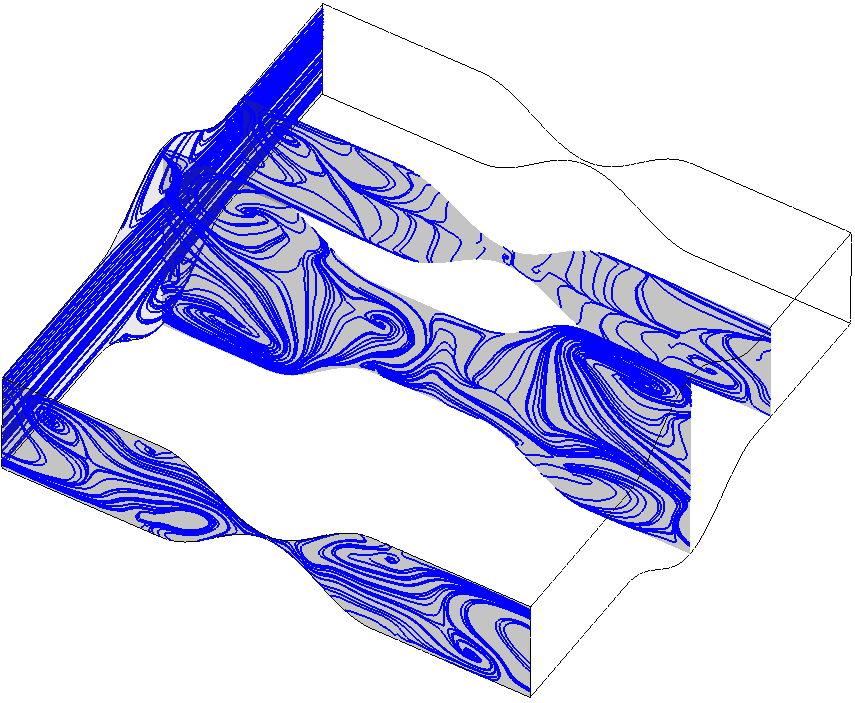
\includegraphics[width=\figuresixpanelwidth]{image_2/Figure7/CA_0deg_2D_stream.png}};
                \begin{scope}[x={(figuresixaimage.south east)},y={(figuresixaimage.north west)}]
                    \node[figuresixcallout] (figuresixwake) at (0.48,0.78)
                        {Wake\\recirculation};
                    \draw[figuresixarrow] (figuresixwake.south west) -- (0.31,0.47);
                \end{scope}
            \end{tikzpicture}\\[-1pt]
            \figuresixlabel{a}{0}
        \end{tabular}%
    }

    \newcommand{\figuresixpanelc}{%
        \begin{tabular}[t]{@{}c@{}}
            \begin{tikzpicture}
                \node[anchor=south west,inner sep=0] (figuresixcimage) at (0,0)
                    {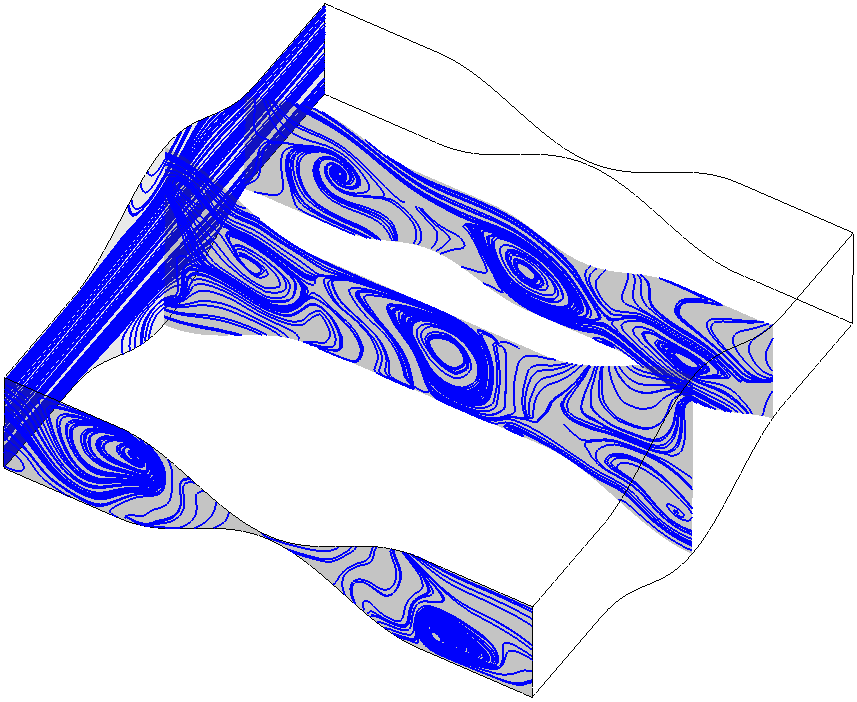
\includegraphics[width=\figuresixpanelwidth]{image_2/Figure7/CA_45deg_2D_stream.png}};
                \begin{scope}[x={(figuresixcimage.south east)},y={(figuresixcimage.north west)}]
                    \node[figuresixcallout] (figuresixreattach) at (0.58,0.79)
                        {Disturbed /\\reattaching flow};
                    \draw[figuresixarrow] (figuresixreattach.south) -- (0.55,0.49);
                \end{scope}
            \end{tikzpicture}\\[-1pt]
            \figuresixlabel{c}{45}
        \end{tabular}%
    }

    \begin{tabular}[c]{@{}c@{\hspace{0.06in}}c@{\hspace{0.06in}}c@{}}
        \figuresixpanela &
        \figuresixpanel{image_2/Figure7/CA_22.5deg_2D_stream.png}{b}{22.5} &
        \figuresixpanelc
    \end{tabular}
    \endgroup
    \caption{2D streamlines of CPHE at representative capsule angles ($\theta_c=0\degree$, $22.5\degree$, and $45\degree$).}
    \label{figure6}
\end{figure}




The field evidence in Figures~\ref{figure5} and~\ref{figure6} explains the nonlinear response in Figure~\ref{figure4}(a). The main transition occurs between $15\degree$ and $22.5\degree$, where Nu increases from 68.87 to 77.04 and $f$ rises from 0.021 to 0.031. The breakup of the streamwise TKE bands and the onset of cross-channel flow through compact recirculation cells increase heat transfer, but the accompanying redirection, separation, and reattachment also increase resistance. From $22.5\degree$ to $45\degree$, the disturbed flow pattern persists and the high-TKE regions broaden. Relative to $0\degree$, Nu and $f$ increase by 23.9\% and 106.3\%, respectively, at $45\degree$. At $22.5\degree$, the corresponding increases are 19.0\% and 93.8\%. The $22.5\degree$ and $45\degree$ cases therefore provide similar heat-transfer--hydraulic trade-offs: $22.5\degree$ marks the main transition in the response, while $45\degree$ gives the maximum Nu of 80.17 with a slightly higher friction factor of 0.033, compared with 0.031 at $22.5\degree$.

\subsubsection{Capsule height}
\label{sec:disc_capsule_height}

Seven capsule heights, $h_c=2.0$--$5.0$~mm in $0.5$~mm increments, are simulated at the fixed capsule angle $\theta_c=22.5\degree$. This corresponds to $h_c/l_c=0.08$--$0.20$. Figures~\ref{figure7} and~\ref{figure8} show representative mid-plane TKE and temperature fields at $h_c/l_c=0.08$, $0.14$, and $0.20$, while Figure~\ref{figure4}(b) reports the friction factor and Nusselt number for the full seven-height sweep.

% Figure 7: editable three-panel LaTeX layout matching Figure 6.
% \figsevenpanelwidth is the final size; no outer scaling is applied.
\begin{figure}[!ht]
    \centering
    \begingroup
    \newlength{\figsevenpanelwidth}
    \newlength{\figsevenlegendunit}
    \setlength{\figsevenpanelwidth}{1.55in}
    \setlength{\figsevenlegendunit}{\dimexpr\figsevenpanelwidth*10/52\relax}

    % Exact RGB values sampled from the updated CFD-Post legend.
    \definecolor{figsevenTKE0}{RGB}{4,41,91}
    \definecolor{figsevenTKE1}{RGB}{27,59,111}
    \definecolor{figsevenTKE2}{RGB}{64,76,108}
    \definecolor{figsevenTKE3}{RGB}{89,95,109}
    \definecolor{figsevenTKE4}{RGB}{111,113,115}
    \definecolor{figsevenTKE5}{RGB}{134,131,120}
    \definecolor{figsevenTKE6}{RGB}{159,150,116}
    \definecolor{figsevenTKE7}{RGB}{184,171,108}
    \definecolor{figsevenTKE8}{RGB}{212,193,92}
    \definecolor{figsevenTKE9}{RGB}{239,217,69}

    \newcommand{\figsevenlegendbar}{%
        \begin{tikzpicture}[baseline=0pt,x=1cm,y=\figsevenlegendunit]
            \fill[figsevenTKE0] (0,0.00) rectangle (0.42,0.52);
            \fill[figsevenTKE1] (0,0.52) rectangle (0.42,1.04);
            \fill[figsevenTKE2] (0,1.04) rectangle (0.42,1.56);
            \fill[figsevenTKE3] (0,1.56) rectangle (0.42,2.08);
            \fill[figsevenTKE4] (0,2.08) rectangle (0.42,2.60);
            \fill[figsevenTKE5] (0,2.60) rectangle (0.42,3.12);
            \fill[figsevenTKE6] (0,3.12) rectangle (0.42,3.64);
            \fill[figsevenTKE7] (0,3.64) rectangle (0.42,4.16);
            \fill[figsevenTKE8] (0,4.16) rectangle (0.42,4.68);
            \fill[figsevenTKE9] (0,4.68) rectangle (0.42,5.20);
            \draw[line width=0.35pt] (0,0) rectangle (0.42,5.20);
            \foreach \y/\ticklabel in {
               0.00/0.0,0.52/1.0,1.04/2.0,1.56/3.0,2.08/4.0,
                2.60/5.0,3.12/6.0,3.64/7.0,4.16/8.0,4.68/9.0,5.20/10.0}
                {\draw[line width=0.3pt] (0.42,\y) -- (0.49,\y)
                 node[anchor=west,font=\sffamily\fontsize{7.5}{8}\selectfont]
                 {\ticklabel};}
        \end{tikzpicture}%
    }

    \newcommand{\figsevenpanellabel}[2]{%
        {\sffamily\bfseries\fontsize{8.5}{9.5}\selectfont
         (#1) $h_c/l_c=#2$}%
    }

    \begin{tabular}[c]{@{}l@{\hspace{0.10in}}c@{\hspace{0.05in}}c@{\hspace{0.05in}}c@{}}
        {\sffamily\bfseries\fontsize{8.5}{9.5}\selectfont
         \shortstack[l]{Turbulence kinetic\\energy, $k$}} & & & \\[-1pt]
        \figsevenlegendbar &
        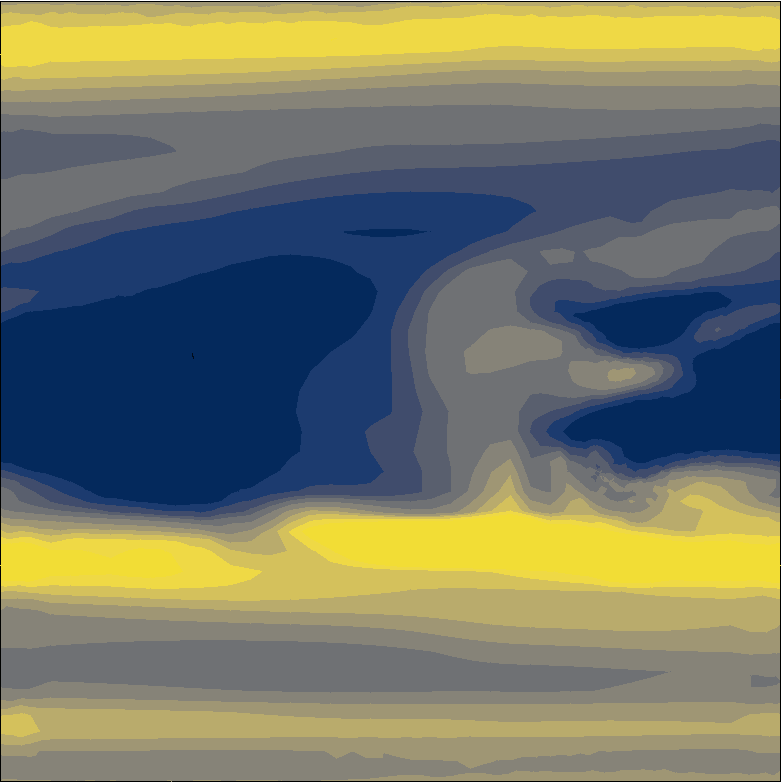
\includegraphics[width=\figsevenpanelwidth]{image_2/Figure9/CH_2mm_TKE.png} &
        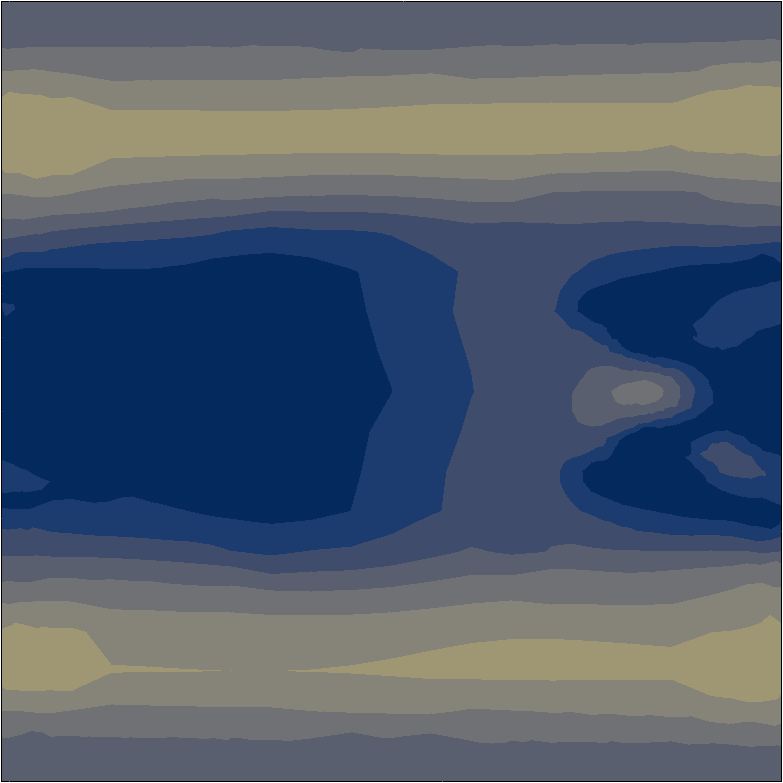
\includegraphics[width=\figsevenpanelwidth]{image_2/Figure9/CH_3.5mm_TKE.png} &
        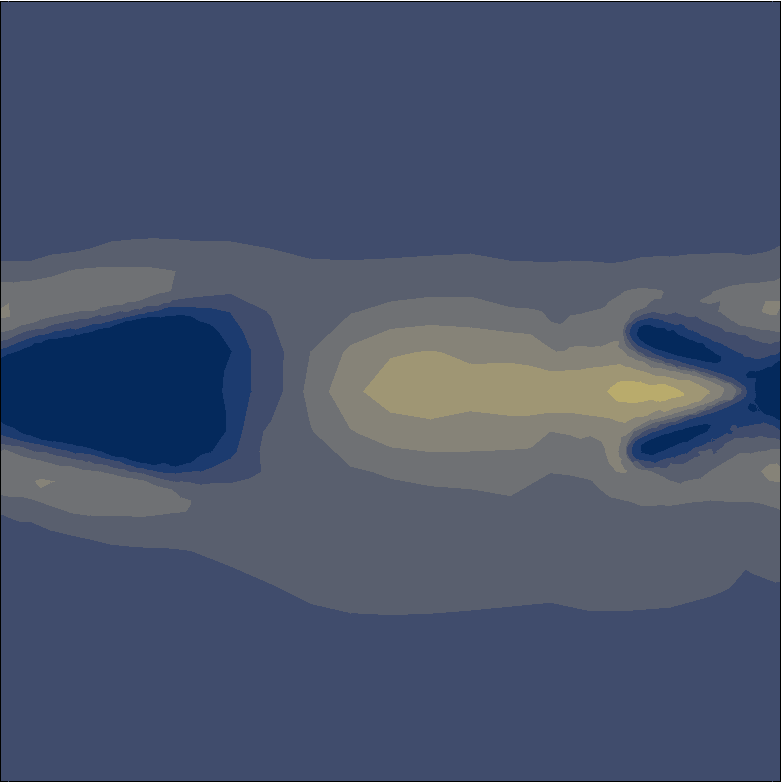
\includegraphics[width=\figsevenpanelwidth]{image_2/Figure9/CH_5mm_TKE.png} \\[-1pt]
        {\sffamily\fontsize{7.5}{8.5}\selectfont
         \shortstack[l]{$\times 10^{-3}$\\$\mathrm{m^2\,s^{-2}}$}} &
        \figsevenpanellabel{a}{0.08} &
        \figsevenpanellabel{b}{0.14} &
        \figsevenpanellabel{c}{0.20}
    \end{tabular}
    \endgroup
    \caption{TKE distribution of the middle $z$-axis section of CPHE at representative normalized capsule heights ($h_c/l_c=0.08$, $0.14$, and $0.20$).}
    \label{figure7}
\end{figure}


Figure~\ref{figure7} shows that capsule height reorganizes the TKE field. At $h_c/l_c=0.08$, high-TKE lanes extend along the outer parts of the section and surround a broad low-TKE wake behind the convex capsule (Figure~\ref{figure7}(a)). At $h_c/l_c=0.14$, these outer lanes weaken and the elevated TKE becomes more localized near the central wake interaction (Figure~\ref{figure7}(b)). At $h_c/l_c=0.20$, low-to-intermediate TKE occupies most of the section and the stronger activity is confined to a compact central wake band (Figure~\ref{figure7}(c)). Increasing height therefore reduces the spatial extent of the highest TKE levels while concentrating the remaining shear near the capsule-induced wake.

% Figure 8: editable three-panel LaTeX layout matching Figure 4.
% \figeightpanelwidth is the final size; no outer scaling is applied.
\begin{figure}[!ht]
    \centering
    \begingroup
    \newlength{\figeightpanelwidth}
    \newlength{\figeightlegendunit}
    \setlength{\figeightpanelwidth}{1.55in}
    \setlength{\figeightlegendunit}{\dimexpr\figeightpanelwidth*10/52\relax}

    \definecolor{figeightTemp0}{RGB}{70,94,207}
    \definecolor{figeightTemp1}{RGB}{103,136,238}
    \definecolor{figeightTemp2}{RGB}{138,173,253}
    \definecolor{figeightTemp3}{RGB}{173,201,253}
    \definecolor{figeightTemp4}{RGB}{205,217,237}
    \definecolor{figeightTemp5}{RGB}{232,214,205}
    \definecolor{figeightTemp6}{RGB}{246,191,166}
    \definecolor{figeightTemp7}{RGB}{244,157,126}
    \definecolor{figeightTemp8}{RGB}{229,112,88}
    \definecolor{figeightTemp9}{RGB}{201,57,54}

    \newcommand{\figeightlegendbar}{%
        \begin{tikzpicture}[baseline=0pt,x=1cm,y=\figeightlegendunit]
            \fill[figeightTemp0] (0,0.00) rectangle (0.42,0.52);
            \fill[figeightTemp1] (0,0.52) rectangle (0.42,1.04);
            \fill[figeightTemp2] (0,1.04) rectangle (0.42,1.56);
            \fill[figeightTemp3] (0,1.56) rectangle (0.42,2.08);
            \fill[figeightTemp4] (0,2.08) rectangle (0.42,2.60);
            \fill[figeightTemp5] (0,2.60) rectangle (0.42,3.12);
            \fill[figeightTemp6] (0,3.12) rectangle (0.42,3.64);
            \fill[figeightTemp7] (0,3.64) rectangle (0.42,4.16);
            \fill[figeightTemp8] (0,4.16) rectangle (0.42,4.68);
            \fill[figeightTemp9] (0,4.68) rectangle (0.42,5.20);
            \draw[line width=0.35pt] (0,0) rectangle (0.42,5.20);
            \foreach \y/\ticklabel in {
                0.00/293,0.52/294,1.04/295,1.56/296,2.08/297,
                2.60/298,3.12/299,3.64/300,4.16/301,4.68/302,5.20/303}
                {\draw[line width=0.3pt] (0.42,\y) -- (0.49,\y)
                 node[anchor=west,font=\sffamily\fontsize{7.5}{8}\selectfont]
                 {\ticklabel};}
        \end{tikzpicture}%
    }

    \newcommand{\figeightpanellabel}[2]{%
        {\sffamily\bfseries\fontsize{8.5}{9.5}\selectfont
         (#1) $h_c/l_c=#2$}%
    }

    \begin{tabular}[c]{@{}l@{\hspace{0.10in}}c@{\hspace{0.05in}}c@{\hspace{0.05in}}c@{}}
        {\sffamily\bfseries\fontsize{8.5}{9.5}\selectfont Temperature} & & & \\[-1pt]
        \figeightlegendbar &
        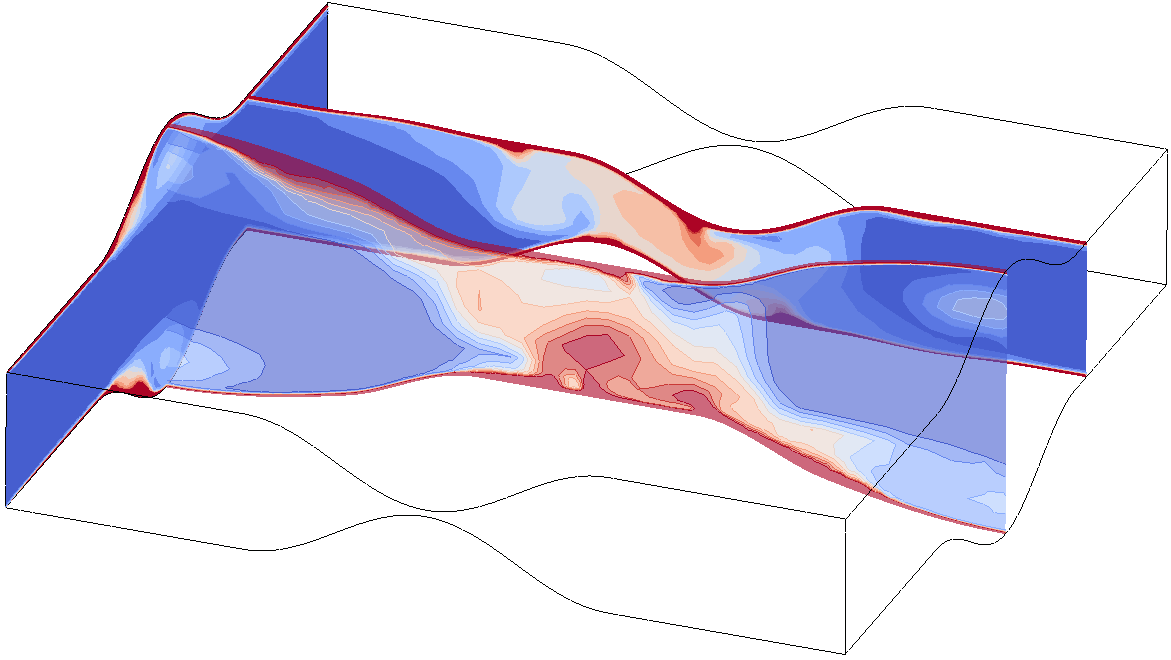
\includegraphics[width=\figeightpanelwidth]{image_2/Figure11/CH_2mm_Temp.png} &
        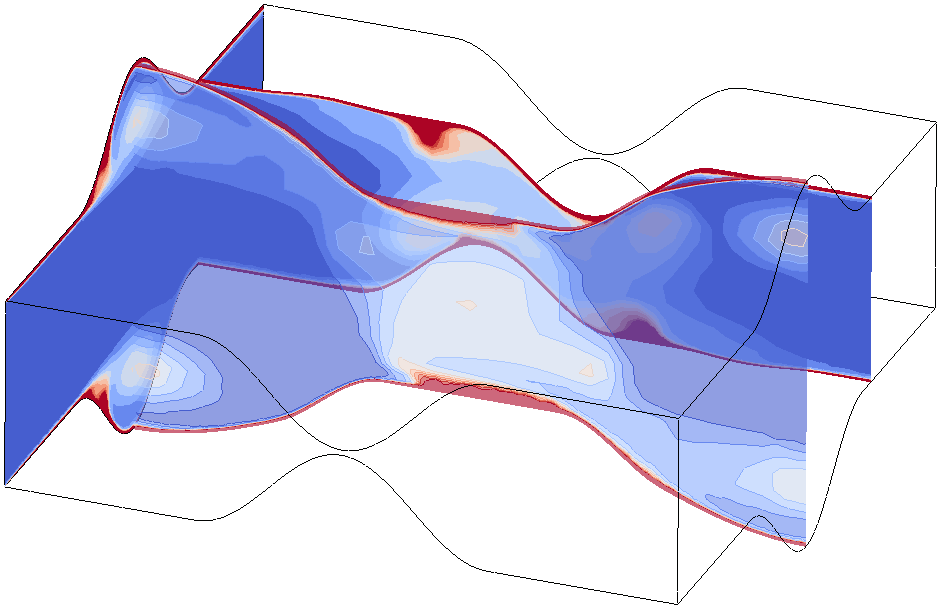
\includegraphics[width=\figeightpanelwidth]{image_2/Figure11/CH_3.5mm_Temp.png} &
        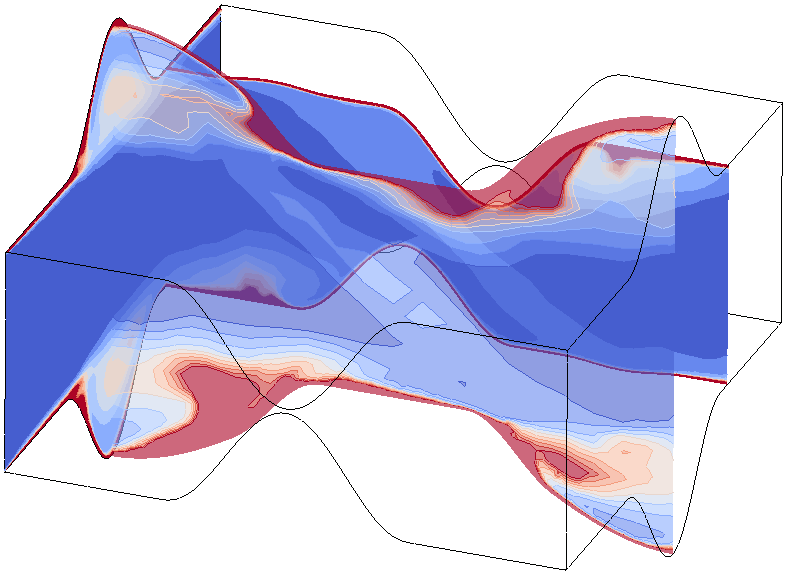
\includegraphics[width=\figeightpanelwidth]{image_2/Figure11/CH_5mm_Temp.png} \\[-1pt]
        {\sffamily\fontsize{7.5}{8.5}\selectfont $[\mathrm{K}]$} &
        \figeightpanellabel{a}{0.08} &
        \figeightpanellabel{b}{0.14} &
        \figeightpanellabel{c}{0.20}
    \end{tabular}
    \endgroup
    \caption{Temperature distribution of CPHE at representative normalized capsule heights ($h_c/l_c=0.08$, $0.14$, and $0.20$).}
    \label{figure8}
\end{figure}


Figure~\ref{figure8} shows the accompanying change in thermal transport. At $h_c/l_c=0.08$, warmer fluid follows the central wake behind the convex capsule (Figure~\ref{figure8}(a)). At $h_c/l_c=0.14$, the warm region is redistributed through the central passage and adjacent concave surfaces (Figure~\ref{figure8}(b)). At $h_c/l_c=0.20$, larger warm regions occupy the concave cavities while the channel core remains cooler (Figure~\ref{figure8}(c)). The main thermal pathway therefore shifts from the convex-capsule wake towards the concave regions as capsule height increases.

The field evidence in Figures~\ref{figure7} and~\ref{figure8} explains the nonlinear response in Figure~\ref{figure4}(b). Increasing capsule height weakens the widespread high-TKE lanes and concentrates the wake interaction, while also moving the warm-fluid pathway towards the concave cavities. These competing changes explain why neither performance measure varies smoothly with height. Nu rises from 69.52 at $h_c/l_c=0.08$ to 77.04 at $0.10$, falls to 75.97 at $0.12$, reaches 80.57 at $0.14$, drops to 75.21 at $0.16$, and then increases to 77.98 at $0.18$ and 86.36 at $0.20$. The friction factor similarly rises from 0.022 at $0.08$ to a local maximum of 0.031 at $0.10$, falls to 0.023 at $0.18$, and rebounds to 0.030 at $0.20$. The localized wake activity and larger warm regions in the $h_c/l_c=0.20$ fields are consistent with the final increase in both Nu and $f$. Across the endpoints, Nu increases by 24.2\% and $f$ by 36.4\%. Within the tested range, $h_c/l_c=0.08$ gives the lowest Nu, $0.18$ gives Nu\,=\,77.98 with the lowest friction factor among the higher-height cases, and $0.20$ gives the maximum Nu with a higher friction penalty.

\subsection{DPHE parametric study}
\label{sec:dphe_results}

Dimple patterns have also been investigated in this study. The DPHE flow-field analysis considers two main parameters: 1) dimple height; and 2) angle of flow.

\subsubsection{Dimple height}
\label{sec:disc_dimple_height}

Seven dimple heights, $h_d=2.0$--$5.0$~mm in $0.5$~mm increments, are simulated at the fixed angle of flow $\theta_d=0\degree$. This corresponds to $h_d/l_d=0.08$--$0.20$. Figures~\ref{figure9} and~\ref{figure10} show representative mid-plane TKE and three-dimensional temperature fields at $h_d/l_d=0.08$, $0.14$, and $0.20$, while Figure~\ref{figure4}(b) reports the friction factor and Nusselt number for the full seven-height sweep.


% \figninepanelwidth is the final size; no outer scaling is applied.
\begin{figure}[!ht]
    \centering
    \begingroup
    \newlength{\figninepanelwidth}
    \newlength{\figninelegendunit}
    \setlength{\figninepanelwidth}{1.55in}
    \setlength{\figninelegendunit}{\dimexpr\figninepanelwidth*10/52\relax}

    
    \definecolor{fignineTKE0}{RGB}{4,41,91}
    \definecolor{fignineTKE1}{RGB}{27,59,111}
    \definecolor{fignineTKE2}{RGB}{64,76,108}
    \definecolor{fignineTKE3}{RGB}{89,95,109}
    \definecolor{fignineTKE4}{RGB}{111,113,115}
    \definecolor{fignineTKE5}{RGB}{134,131,120}
    \definecolor{fignineTKE6}{RGB}{159,150,116}
    \definecolor{fignineTKE7}{RGB}{184,171,108}
    \definecolor{fignineTKE8}{RGB}{212,193,92}
    \definecolor{fignineTKE9}{RGB}{239,217,69}

    \newcommand{\figninelegendbar}{%
        \begin{tikzpicture}[baseline=0pt,x=1cm,y=\figninelegendunit]
            \fill[fignineTKE0] (0,0.00) rectangle (0.42,0.52);
            \fill[fignineTKE1] (0,0.52) rectangle (0.42,1.04);
            \fill[fignineTKE2] (0,1.04) rectangle (0.42,1.56);
            \fill[fignineTKE3] (0,1.56) rectangle (0.42,2.08);
            \fill[fignineTKE4] (0,2.08) rectangle (0.42,2.60);
            \fill[fignineTKE5] (0,2.60) rectangle (0.42,3.12);
            \fill[fignineTKE6] (0,3.12) rectangle (0.42,3.64);
            \fill[fignineTKE7] (0,3.64) rectangle (0.42,4.16);
            \fill[fignineTKE8] (0,4.16) rectangle (0.42,4.68);
            \fill[fignineTKE9] (0,4.68) rectangle (0.42,5.20);
            \draw[line width=0.35pt] (0,0) rectangle (0.42,5.20);
            \foreach \y/\ticklabel in {
                0.00/0.0,0.52/1.0,1.04/2.0,1.56/3.0,2.08/4.0,
                2.60/5.0,3.12/6.0,3.64/7.0,4.16/8.0,4.68/9.0,5.20/10.0}
                {\draw[line width=0.3pt] (0.42,\y) -- (0.49,\y)
                 node[anchor=west,font=\sffamily\fontsize{7.5}{8}\selectfont]
                 {\ticklabel};}
        \end{tikzpicture}%
    }

    \newcommand{\figninepanellabel}[2]{%
        {\sffamily\bfseries\fontsize{8.5}{9.5}\selectfont
         (#1) $h_d/l_d=#2$}%
    }

    \begin{tabular}[c]{@{}l@{\hspace{0.10in}}c@{\hspace{0.05in}}c@{\hspace{0.05in}}c@{}}
        {\sffamily\bfseries\fontsize{8.5}{9.5}\selectfont
         \shortstack[l]{Turbulence kinetic\\energy, $k$}} & & & \\[-1pt]
        \figninelegendbar &
        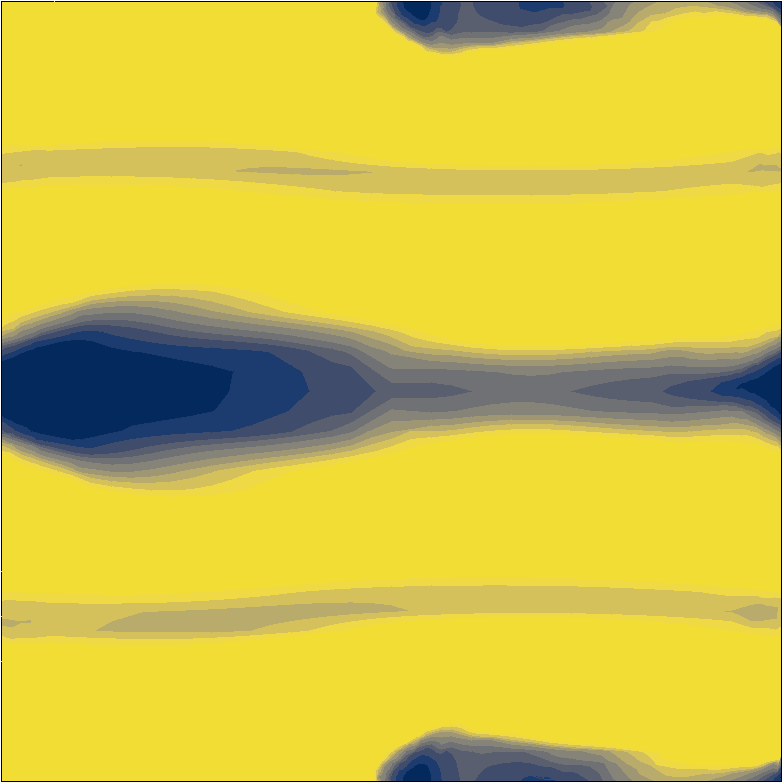
\includegraphics[width=\figninepanelwidth]{image_2/Figure12/DH_2mm_TKE.png} &
        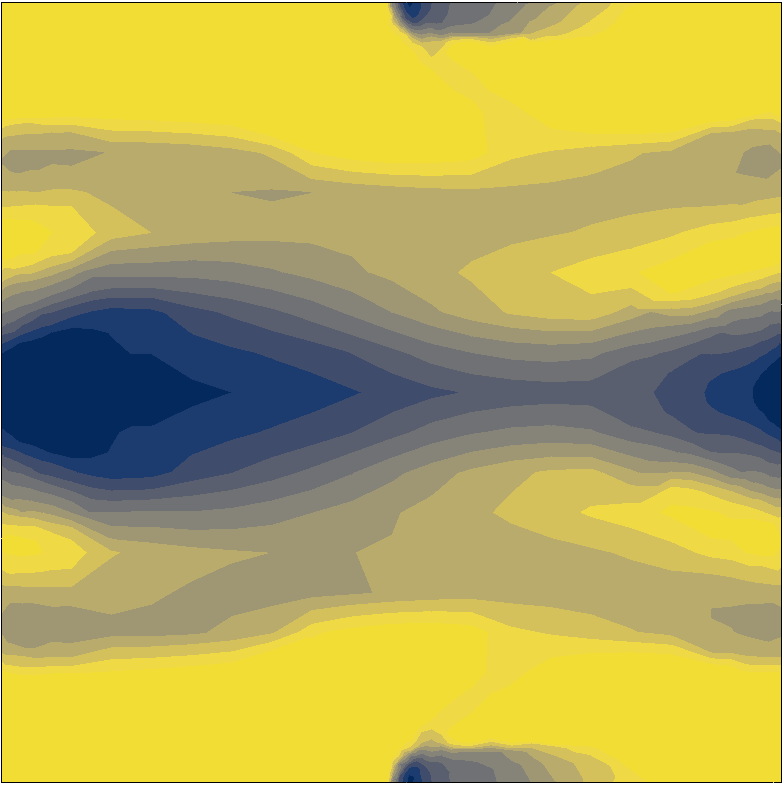
\includegraphics[width=\figninepanelwidth]{image_2/Figure12/DH_3.5mm_TKE.png} &
        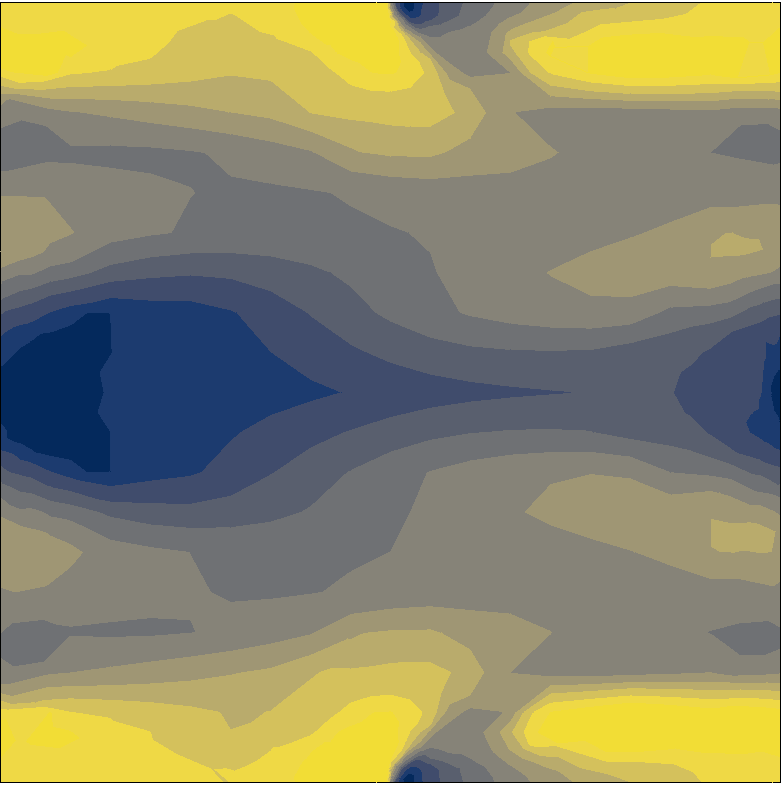
\includegraphics[width=\figninepanelwidth]{image_2/Figure12/DH_5mm_TKE.png} \\[-1pt]
        {\sffamily\fontsize{7.5}{8.5}\selectfont
         \shortstack[l]{$\times 10^{-3}$\\$\mathrm{m^2\,s^{-2}}$}} &
        \figninepanellabel{a}{0.08} &
        \figninepanellabel{b}{0.14} &
        \figninepanellabel{c}{0.20}
    \end{tabular}
    \endgroup
    \caption{TKE distribution of the middle $z$-axis section of DPHE at representative normalized dimple heights ($h_d/l_d=0.08$, $0.14$, and $0.20$).}
    \label{figure9}
\end{figure}


Figure~\ref{figure9} shows that dimple height reorganizes the TKE field rather than increasing its magnitude uniformly. At $h_d/l_d=0.08$ (Figure~\ref{figure9}(a)), high TKE occupies most of the section and encloses a long, low-TKE wake through the centre. At $h_d/l_d=0.14$ (Figure~\ref{figure9}(b)), the high-TKE field recedes from the central passage and becomes more concentrated near the outer shear regions, while the low-TKE wake remains surrounded by a broader intermediate-TKE transition. At $h_d/l_d=0.20$ (Figure~\ref{figure9}(c)), low-to-intermediate TKE occupies most of the central passage and the highest TKE is confined mainly to narrow regions near the dimple rims and outer boundaries. Increasing $h_d$ therefore localizes the strongest shear and reshapes the wake interaction instead of producing a section-wide rise in TKE.

% Figure 10: editable LaTeX layout matching Figure 9.
% \figtenpanelwidth is the final size; no outer scaling is applied.
\begin{figure}[!ht]
    \centering
    \begingroup
    \newlength{\figtenpanelwidth}
    \newlength{\figtenlegendunit}
    \setlength{\figtenpanelwidth}{1.55in}
    \setlength{\figtenlegendunit}{\dimexpr\figtenpanelwidth*10/52\relax}

    % Exact RGB values sampled from the updated CFD-Post legend.
    \definecolor{figtenTemp0}{RGB}{70,94,207}
    \definecolor{figtenTemp1}{RGB}{103,136,238}
    \definecolor{figtenTemp2}{RGB}{138,173,253}
    \definecolor{figtenTemp3}{RGB}{173,201,253}
    \definecolor{figtenTemp4}{RGB}{205,217,237}
    \definecolor{figtenTemp5}{RGB}{232,214,205}
    \definecolor{figtenTemp6}{RGB}{246,191,166}
    \definecolor{figtenTemp7}{RGB}{244,157,126}
    \definecolor{figtenTemp8}{RGB}{229,112,88}
    \definecolor{figtenTemp9}{RGB}{201,57,54}

    \newcommand{\figtenlegendbar}{%
        \begin{tikzpicture}[baseline=0pt,x=1cm,y=\figtenlegendunit]
            \fill[figtenTemp0] (0,0.00) rectangle (0.42,0.52);
            \fill[figtenTemp1] (0,0.52) rectangle (0.42,1.04);
            \fill[figtenTemp2] (0,1.04) rectangle (0.42,1.56);
            \fill[figtenTemp3] (0,1.56) rectangle (0.42,2.08);
            \fill[figtenTemp4] (0,2.08) rectangle (0.42,2.60);
            \fill[figtenTemp5] (0,2.60) rectangle (0.42,3.12);
            \fill[figtenTemp6] (0,3.12) rectangle (0.42,3.64);
            \fill[figtenTemp7] (0,3.64) rectangle (0.42,4.16);
            \fill[figtenTemp8] (0,4.16) rectangle (0.42,4.68);
            \fill[figtenTemp9] (0,4.68) rectangle (0.42,5.20);
            \draw[line width=0.35pt] (0,0) rectangle (0.42,5.20);
            \foreach \y/\ticklabel in {
                0.00/293,0.52/294,1.04/295,1.56/296,2.08/297,
                2.60/298,3.12/299,3.64/300,4.16/301,4.68/302,5.20/303}
                {\draw[line width=0.3pt] (0.42,\y) -- (0.49,\y)
                 node[anchor=west,font=\sffamily\fontsize{7.5}{8}\selectfont]
                 {\ticklabel};}
        \end{tikzpicture}%
    }

    \newcommand{\figtenpanellabel}[2]{%
        {\sffamily\bfseries\fontsize{8.5}{9.5}\selectfont
         (#1) $h_d/l_d=#2$}%
    }

    \begin{tabular}[c]{@{}l@{\hspace{0.10in}}c@{\hspace{0.05in}}c@{\hspace{0.05in}}c@{}}
        {\sffamily\bfseries\fontsize{8.5}{9.5}\selectfont Temperature} & & & \\[-1pt]
        \figtenlegendbar &
        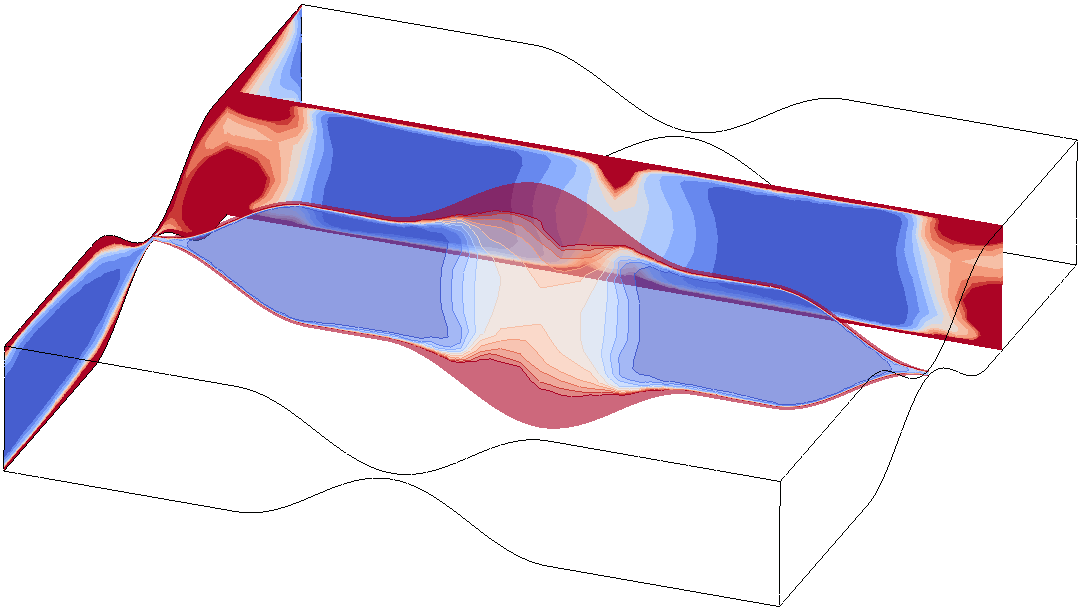
\includegraphics[width=\figtenpanelwidth]{image_2/Figure14/DH_2mm_Temp.png} &
        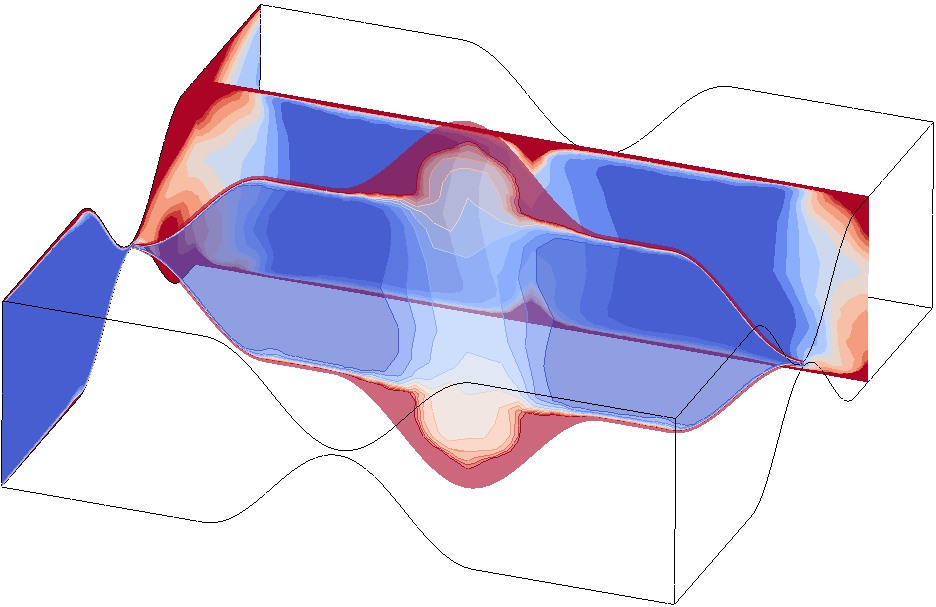
\includegraphics[width=\figtenpanelwidth]{image_2/Figure14/DH_3.5mm_Temp.png} &
        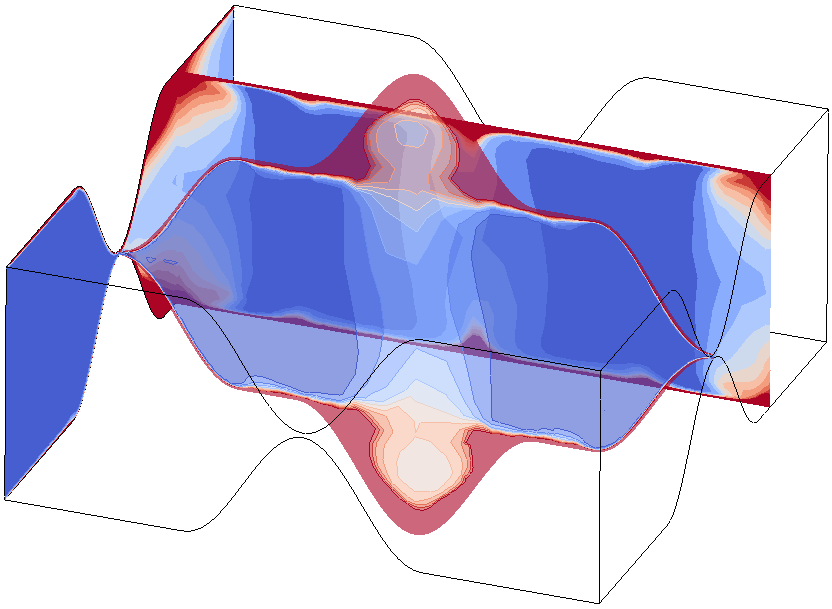
\includegraphics[width=\figtenpanelwidth]{image_2/Figure14/DH_5mm_Temp.png} \\[-1pt]
        {\sffamily\fontsize{7.5}{8.5}\selectfont $[\mathrm{K}]$} &
        \figtenpanellabel{a}{0.08} &
        \figtenpanellabel{b}{0.14} &
        \figtenpanellabel{c}{0.20}
    \end{tabular}
    \endgroup
    \caption{3D temperature distribution of DPHE at representative normalized dimple heights ($h_d/l_d=0.08$, $0.14$, and $0.20$).}
    \label{figure10}
\end{figure}


Figure~\ref{figure10} provides the corresponding thermal evidence. At $h_d/l_d=0.08$ (Figure~\ref{figure10}(a)), the warmed-fluid region is comparatively compact around the central dimple and much of the channel core remains cool. At $h_d/l_d=0.14$ (Figure~\ref{figure10}(b)), the thermal plume projects farther across the passage and occupies more of the region between the opposing embossed surfaces. At $h_d/l_d=0.20$ (Figure~\ref{figure10}(c)), this plume is largest and penetrates farthest into the channel, while the warm regions around the upper and lower dimples are more developed. The progressive growth of this thermal footprint indicates stronger wall-to-core energy transport as dimple height increases.

The field evidence in Figures~\ref{figure9} and~\ref{figure10} explains the monotonic response in Figure~\ref{figure4}(b). As $h_d/l_d$ increases from 0.08 to 0.20, the friction factor rises from approximately 0.025 to 0.071 and Nu increases from approximately 55 to 99. The wake reorganization and localization of the strongest shear near the dimple rims in Figure~\ref{figure9} are consistent with the greater hydraulic resistance produced as taller dimples redirect the flow more strongly. At the same time, the expanding thermal plume in Figure~\ref{figure10} demonstrates increased exchange between the heated surfaces and the cooler channel core, accounting for the rise in Nu. The reduction in the spatial extent of the highest TKE levels does not contradict the heat-transfer trend: the performance gain is governed by where shear and thermal transport occur, rather than by a uniform increase in TKE throughout the section. Consequently, $h_d/l_d=0.08$--$0.10$ minimizes resistance but gives the lowest Nu, $0.18$--$0.20$ maximizes heat transfer with the largest friction penalty, and $0.12$--$0.16$ provides an intermediate trade-off.

\subsubsection{Dimple angle}
\label{sec:disc_dimple_angle}

Although each circular dimple is axisymmetric, changing the angle of flow relative to the dimple array changes how the wakes generated by neighboring convex and concave features intersect \citep{jiang2019a, hamedi2024}. Seven angles, $\theta_d=0\degree$--$45\degree$ in $7.5\degree$ increments, are simulated. Figure~\ref{figure11} presents representative mid-plane TKE fields at $\theta_d=0\degree$, $22.5\degree$, and $45\degree$. At $0\degree$ (Figure~\ref{figure11}(a)), a broad, nearly symmetric low-TKE corridor spans the centre of the unit cell, separating the energetic regions on either side. At $22.5\degree$ (Figure~\ref{figure11}(b)), this symmetry is broken: the low-TKE region rotates into an oblique wake and is bordered by a concentrated high-TKE band. At $45\degree$ (Figure~\ref{figure11}(c)), the field is reorganized into a coherent diagonal corridor of low-to-intermediate TKE, with the highest TKE confined to narrower regions near the dimples. The angle of flow therefore produces a non-monotonic redistribution of turbulence rather than a uniform increase or decrease in TKE.



\begin{figure}[!ht]
    \centering
    \begingroup
    \newlength{\figelevenpanelwidth}
    \newlength{\figelevenlegendunit}
    \setlength{\figelevenpanelwidth}{1.55in}
    \setlength{\figelevenlegendunit}{\dimexpr\figelevenpanelwidth*10/52\relax}

  
    \definecolor{figelevenTKE0}{RGB}{4,41,91}
    \definecolor{figelevenTKE1}{RGB}{27,59,111}
    \definecolor{figelevenTKE2}{RGB}{64,76,108}
    \definecolor{figelevenTKE3}{RGB}{89,95,109}
    \definecolor{figelevenTKE4}{RGB}{111,113,115}
    \definecolor{figelevenTKE5}{RGB}{134,131,120}
    \definecolor{figelevenTKE6}{RGB}{159,150,116}
    \definecolor{figelevenTKE7}{RGB}{184,171,108}
    \definecolor{figelevenTKE8}{RGB}{212,193,92}
    \definecolor{figelevenTKE9}{RGB}{239,217,69}

    \newcommand{\figelevenlegendbar}{%
        \begin{tikzpicture}[baseline=0pt,x=1cm,y=\figelevenlegendunit]
            \fill[figelevenTKE0] (0,0.00) rectangle (0.42,0.52);
            \fill[figelevenTKE1] (0,0.52) rectangle (0.42,1.04);
            \fill[figelevenTKE2] (0,1.04) rectangle (0.42,1.56);
            \fill[figelevenTKE3] (0,1.56) rectangle (0.42,2.08);
            \fill[figelevenTKE4] (0,2.08) rectangle (0.42,2.60);
            \fill[figelevenTKE5] (0,2.60) rectangle (0.42,3.12);
            \fill[figelevenTKE6] (0,3.12) rectangle (0.42,3.64);
            \fill[figelevenTKE7] (0,3.64) rectangle (0.42,4.16);
            \fill[figelevenTKE8] (0,4.16) rectangle (0.42,4.68);
            \fill[figelevenTKE9] (0,4.68) rectangle (0.42,5.20);
            \draw[line width=0.35pt] (0,0) rectangle (0.42,5.20);
            \foreach \y/\ticklabel in {
                0.00/0.0,0.52/1.0,1.04/2.0,1.56/3.0,2.08/4.0,
                2.60/5.0,3.12/6.0,3.64/7.0,4.16/8.0,4.68/9.0,5.20/10.0}
                {\draw[line width=0.3pt] (0.42,\y) -- (0.49,\y)
                 node[anchor=west,font=\sffamily\fontsize{7.5}{8}\selectfont]
                 {\ticklabel};}
        \end{tikzpicture}%
    }

    \newcommand{\figelevenpanellabel}[2]{%
        {\sffamily\bfseries\fontsize{8.5}{9.5}\selectfont
         (#1) $\theta_d=#2\degree$}%
    }

    \begin{tabular}[c]{@{}l@{\hspace{0.10in}}c@{\hspace{0.05in}}c@{\hspace{0.05in}}c@{}}
        {\sffamily\bfseries\fontsize{8.5}{9.5}\selectfont
         \shortstack[l]{Turbulence kinetic\\energy, $k$}} & & & \\[-1pt]
        \figelevenlegendbar &
        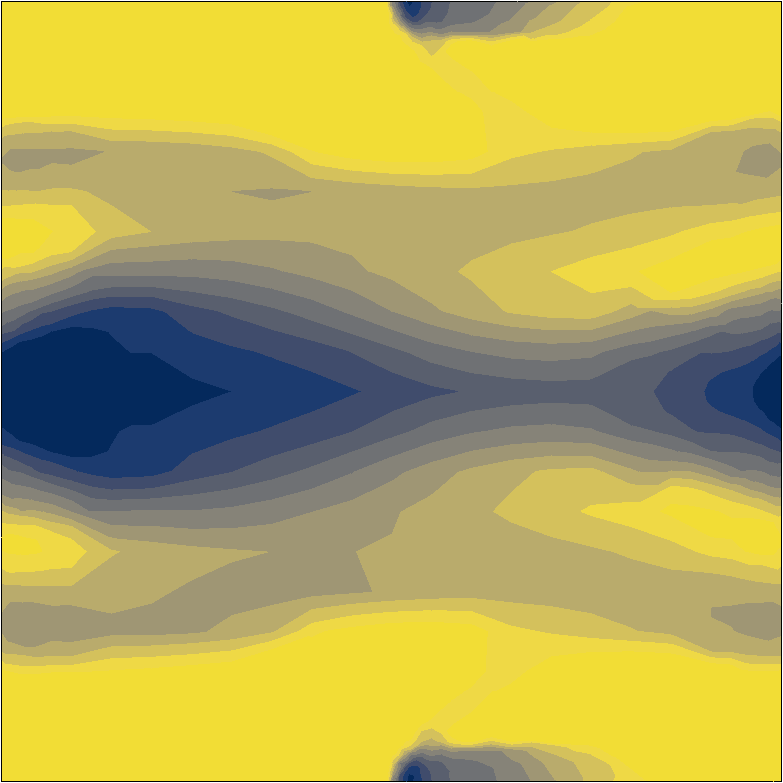
\includegraphics[width=\figelevenpanelwidth]{image_2/Figure15/DA_0deg_TKE.png} &
        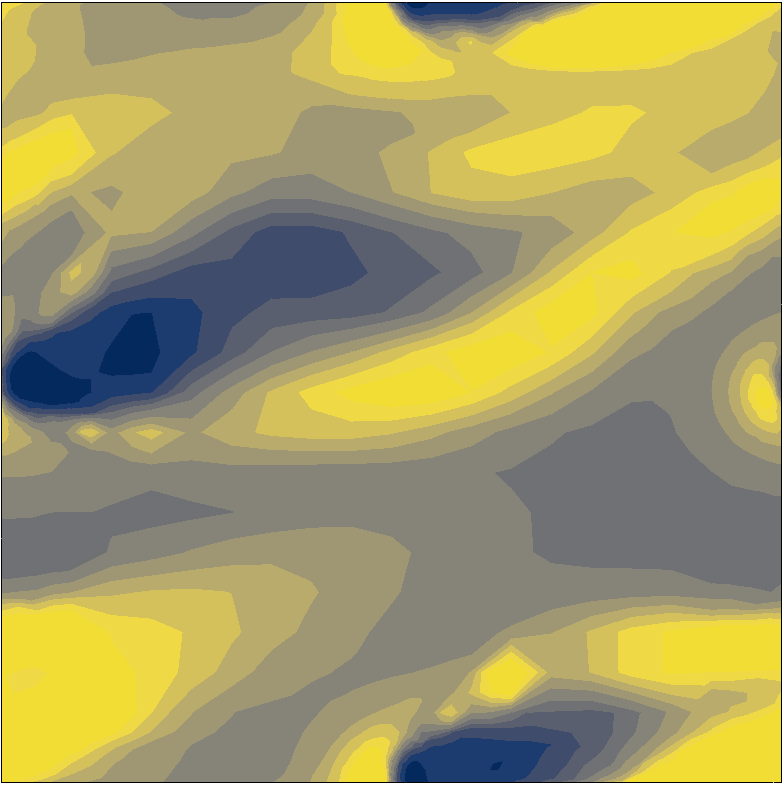
\includegraphics[width=\figelevenpanelwidth]{image_2/Figure15/DA_22.5deg_TKE.png} &
        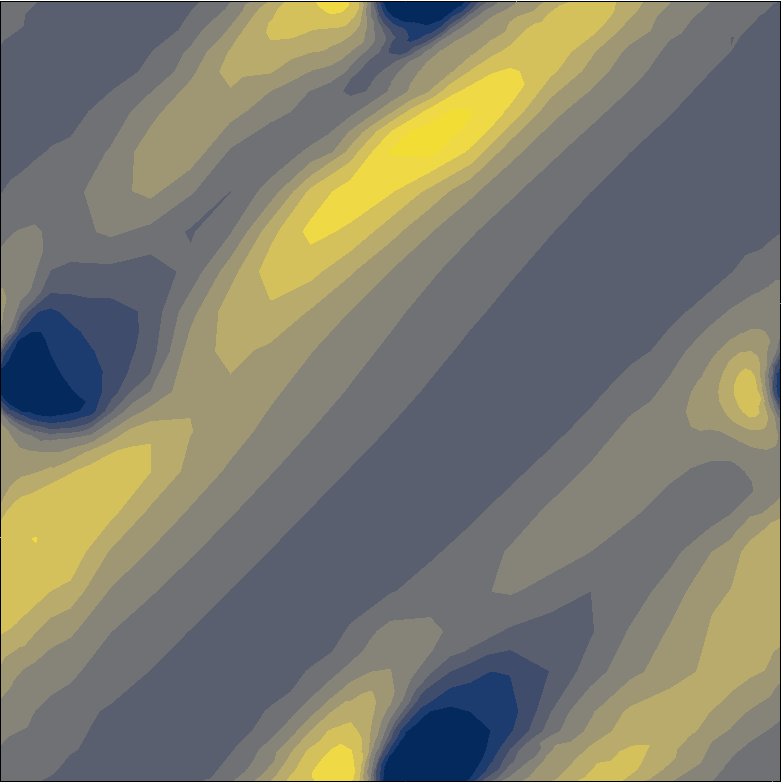
\includegraphics[width=\figelevenpanelwidth]{image_2/Figure15/DA_45deg_TKE.png} \\[-1pt]
        {\sffamily\fontsize{7.5}{8.5}\selectfont
         \shortstack[l]{$\times 10^{-3}$\\$\mathrm{m^2\,s^{-2}}$}} &
        \figelevenpanellabel{a}{0} &
        \figelevenpanellabel{b}{22.5} &
        \figelevenpanellabel{c}{45}
    \end{tabular}
    \endgroup
    \caption{TKE distribution of the middle $z$-axis section of DPHE at representative angles of flow ($\theta_d=0\degree$, $22.5\degree$, and $45\degree$).}
    \label{figure11}
\end{figure}


\begin{figure}[!ht]
    \centering
    \begingroup
    \newlength{\figtwelvepanelwidth}
    \setlength{\figtwelvepanelwidth}{0.31\textwidth}

    \newcommand{\figtwelvelabel}[2]{%
        {\sffamily\bfseries\fontsize{8.5}{9.5}\selectfont
         (#1) $\theta_d=#2\degree$}%
    }

    \newcommand{\figtwelvepanel}[3]{%
        \begin{tabular}[t]{@{}c@{}}
            \includegraphics[width=\figtwelvepanelwidth]{#1}\\[-1pt]
            \figtwelvelabel{#2}{#3}
        \end{tabular}%
    }

    \begin{tabular}[c]{@{}c@{\hspace{0.05in}}c@{\hspace{0.05in}}c@{}}
        \figtwelvepanel{image_2/Figure16/DA_0deg_2D_stream.png}{a}{0} &
        \figtwelvepanel{image_2/Figure16/DA_22.5deg_2D_stream.png}{b}{22.5} &
        \figtwelvepanel{image_2/Figure16/DA_45deg_2D_stream.png}{c}{45}
    \end{tabular}
    \endgroup
    \caption{2D streamlines of DPHE at representative angles of flow ($\theta_d=0\degree$, $22.5\degree$, and $45\degree$).}
    \label{figure12}
\end{figure}


The streamline fields in Figure~\ref{figure12} provide the corresponding flow-topology evidence. At $0\degree$ (Figure~\ref{figure12}(a)), numerous compact recirculation cells are distributed through the central interaction region and the dimple cavities; much of this secondary motion remains locally confined. At $22.5\degree$ (Figure~\ref{figure12}(b)), the cells consolidate into larger structures and interact with an oblique through-flow passage, strengthening the exchange between the dimple wakes and the channel flow. At $45\degree$ (Figure~\ref{figure12}(c)), long, nearly parallel streamlines dominate the diagonal passage, while recirculation is restricted mainly to elongated pockets beside the central dimple and smaller cells near the outer cavities. This progression is consistent with the TKE redistribution in Figure~\ref{figure11}: the intermediate angle couples the energetic wake band to the through-flow, whereas the largest angle establishes a more coherent passage that bypasses much of the strongest wake interaction.

The flow-field evidence in Figures~\ref{figure11} and~\ref{figure12} explains the non-monotonic performance response in Figure~\ref{figure4}(a). From $0\degree$ to the intermediate-angle range, the friction factor rises from approximately 0.051 to 0.064--0.065, while Nu increases from approximately 81 to 94--98 and reaches its maximum near $30\degree$. The breakup of the symmetric low-TKE corridor, formation of the oblique high-TKE band, and stronger interaction between recirculation and through-flow promote wall-to-core mixing and heat transfer, but also increase shear and flow resistance. Beyond $30\degree$, both quantities fall sharply; at $45\degree$, $f$ is approximately 0.021 and Nu is approximately 70. The diagonal low-to-intermediate-TKE corridor in Figure~\ref{figure11}(c), together with the predominantly parallel streamlines in Figure~\ref{figure12}(c), shows why: the flow is channelled through a coherent oblique passage, reducing wake-driven mixing and the associated hydraulic penalty. Accordingly, angles of approximately $15\degree$--$30\degree$ favour heat transfer at the cost of higher resistance, whereas $37.5\degree$--$45\degree$ reduce resistance but also substantially reduce Nu.

\subsection{Cross-parameter thermo-geometric comparison}
\label{sec:tgg_comparison}

Figures~\ref{figure13} and~\ref{figure14} isolate PEC for the angle and normalized-height sweeps introduced in Figure~\ref{figure4}. Figure~\ref{figure15} then compares the 28 one-factor cases and the targeted combined dimple case using PEC (Equation~\eqref{eq:PEC}) and RED (Equation~\eqref{eq:red}). Figure~\ref{figure13} shows that $\theta_d=45\degree$ gives the highest PEC among the original dimple-angle cases, following the sharp reduction in $f$ discussed in Section~\ref{sec:disc_dimple_angle}. The targeted case therefore combines $\theta_d=45\degree$ with $h_d=5.0$~mm instead of the angle sweep's fixed $h_d=3.5$~mm.

\noindent% Figure 13: focused PEC comparison for the angle sweeps.
\begin{minipage}[t]{0.485\linewidth}
    \centering
    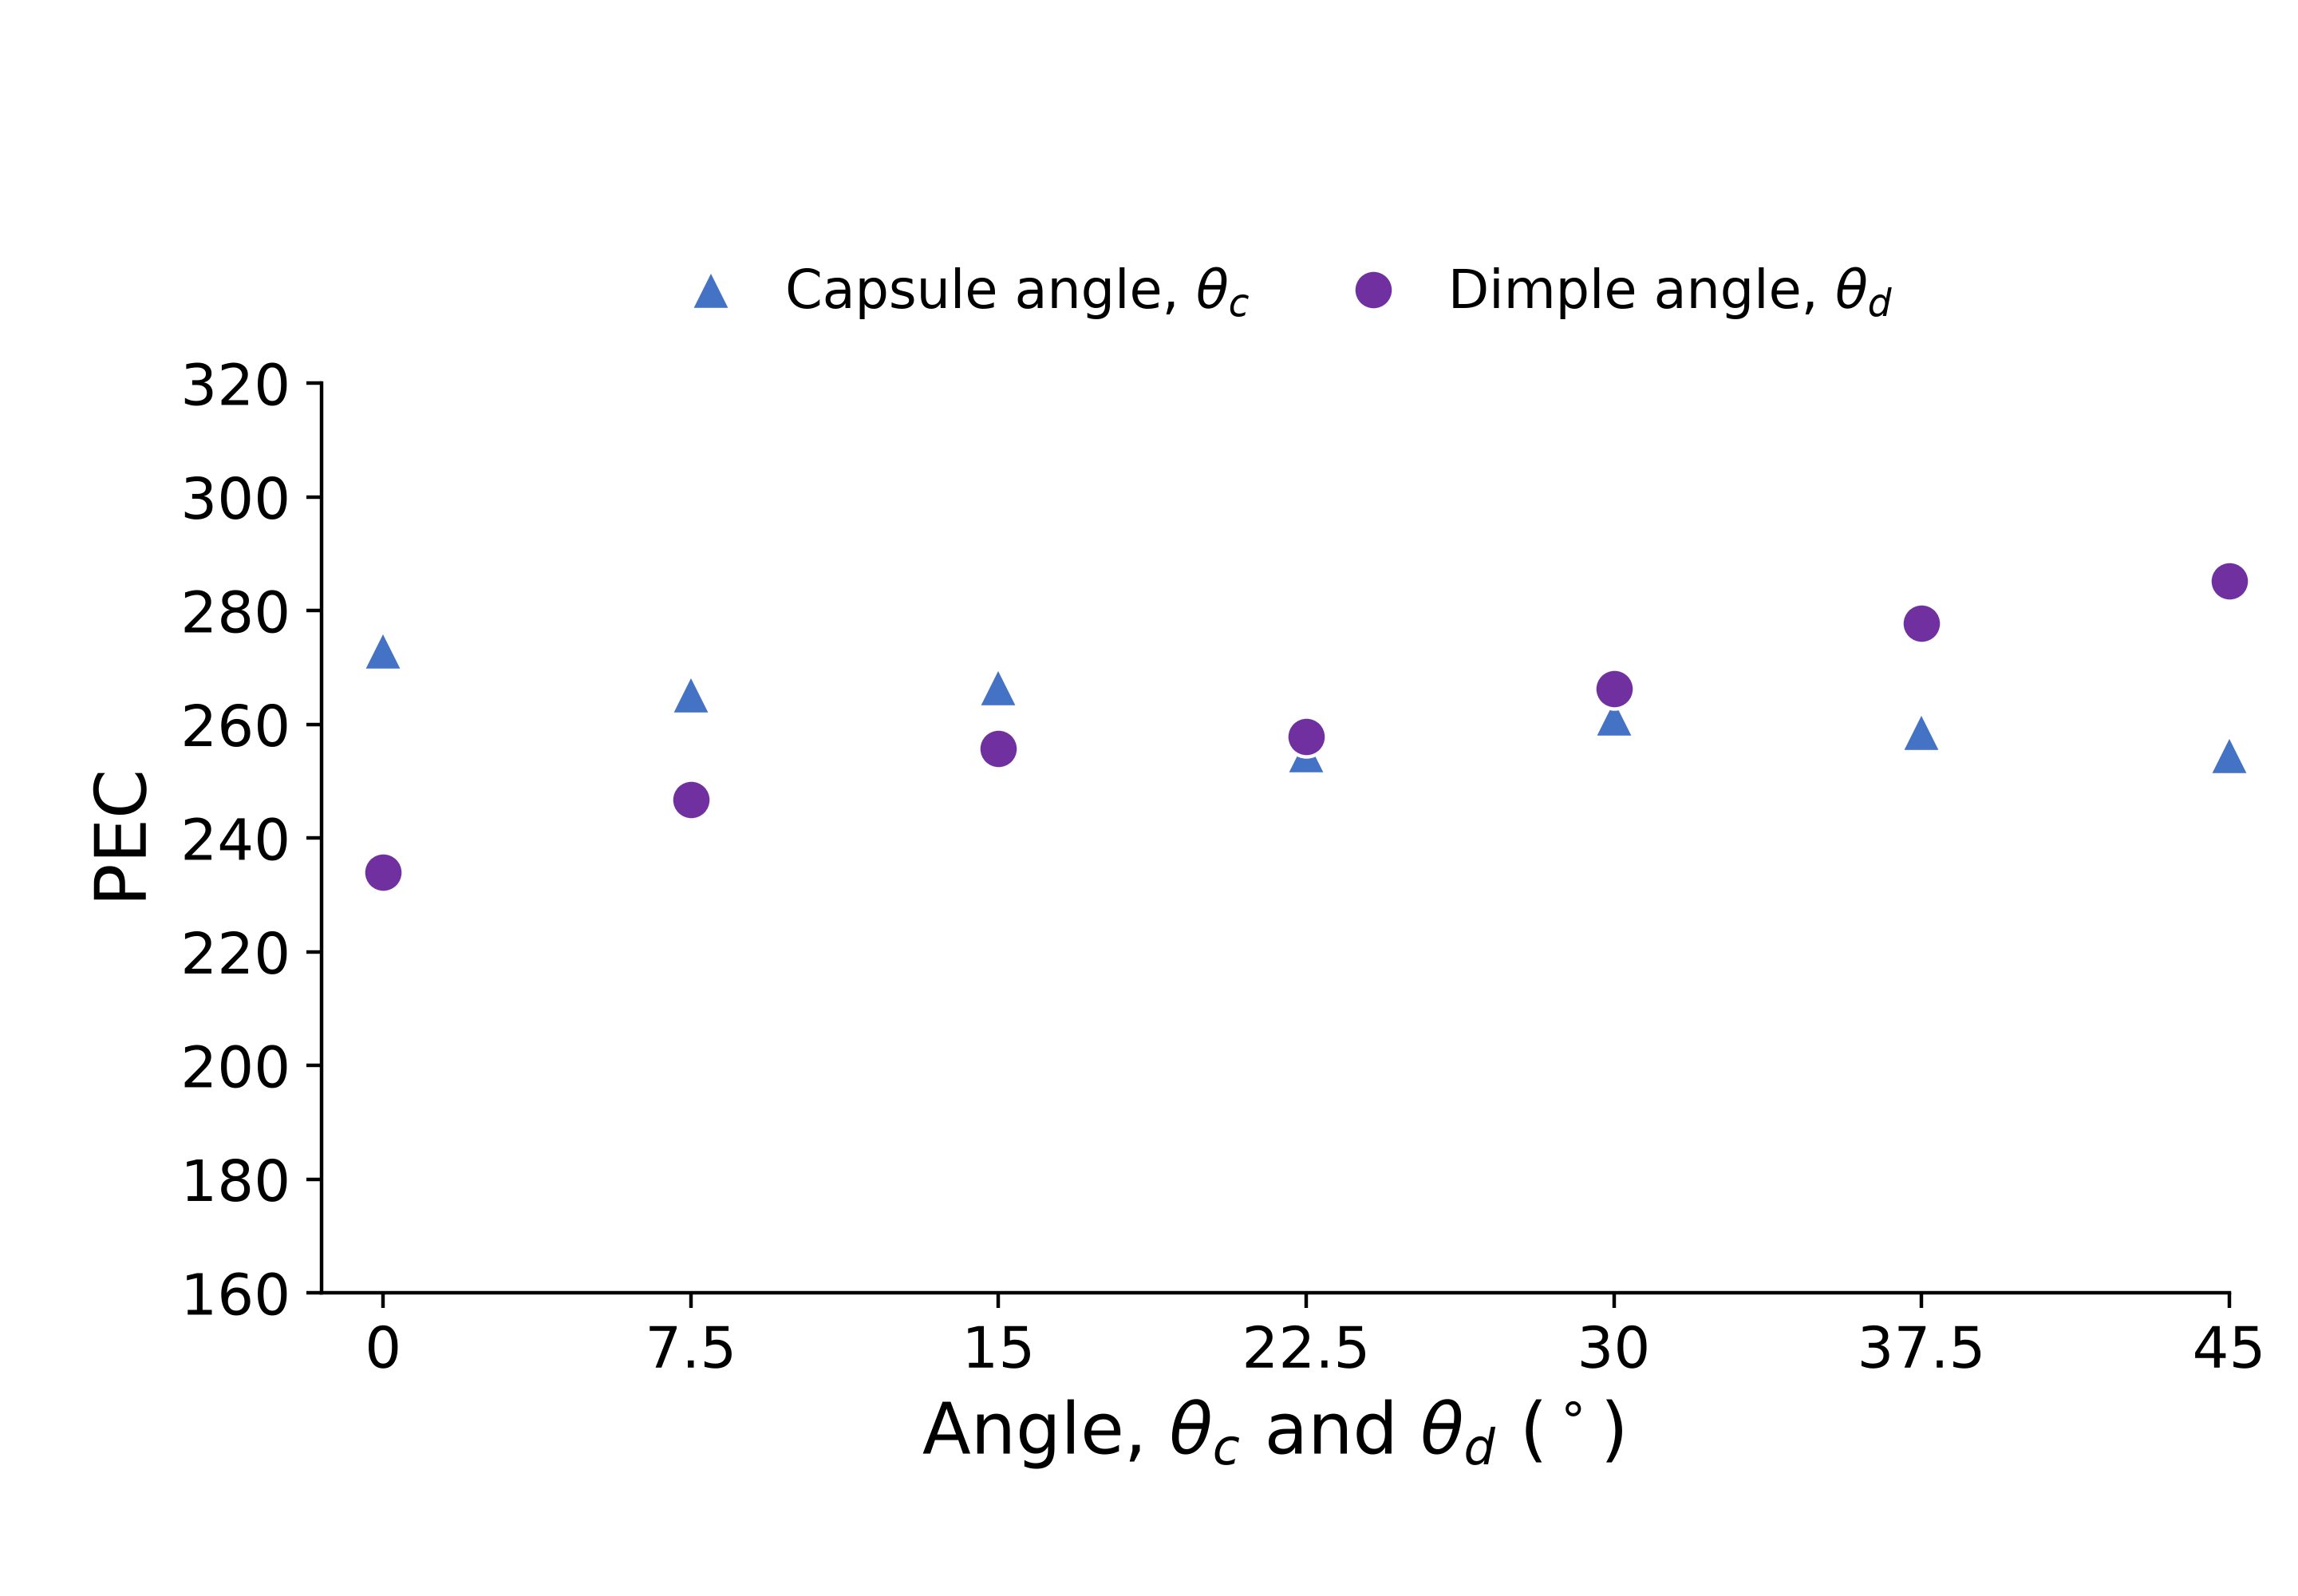
\includegraphics[
        width=\linewidth,
        keepaspectratio,
        interpolate=true
    ]{media/Figure13_PEC_angle.png}
    \captionsetup{hypcap=false}
    \captionof{figure}{Two-wall PEC referenced to the fluid-domain mass-average temperature for the angle sweeps: $h_c=2.5$~mm and $h_d=3.5$~mm.}
    \label{figure13}
\end{minipage}%
\hfill% Figure 14: focused PEC comparison for the normalized-height sweeps.
\begin{minipage}[t]{0.485\linewidth}
    \centering
    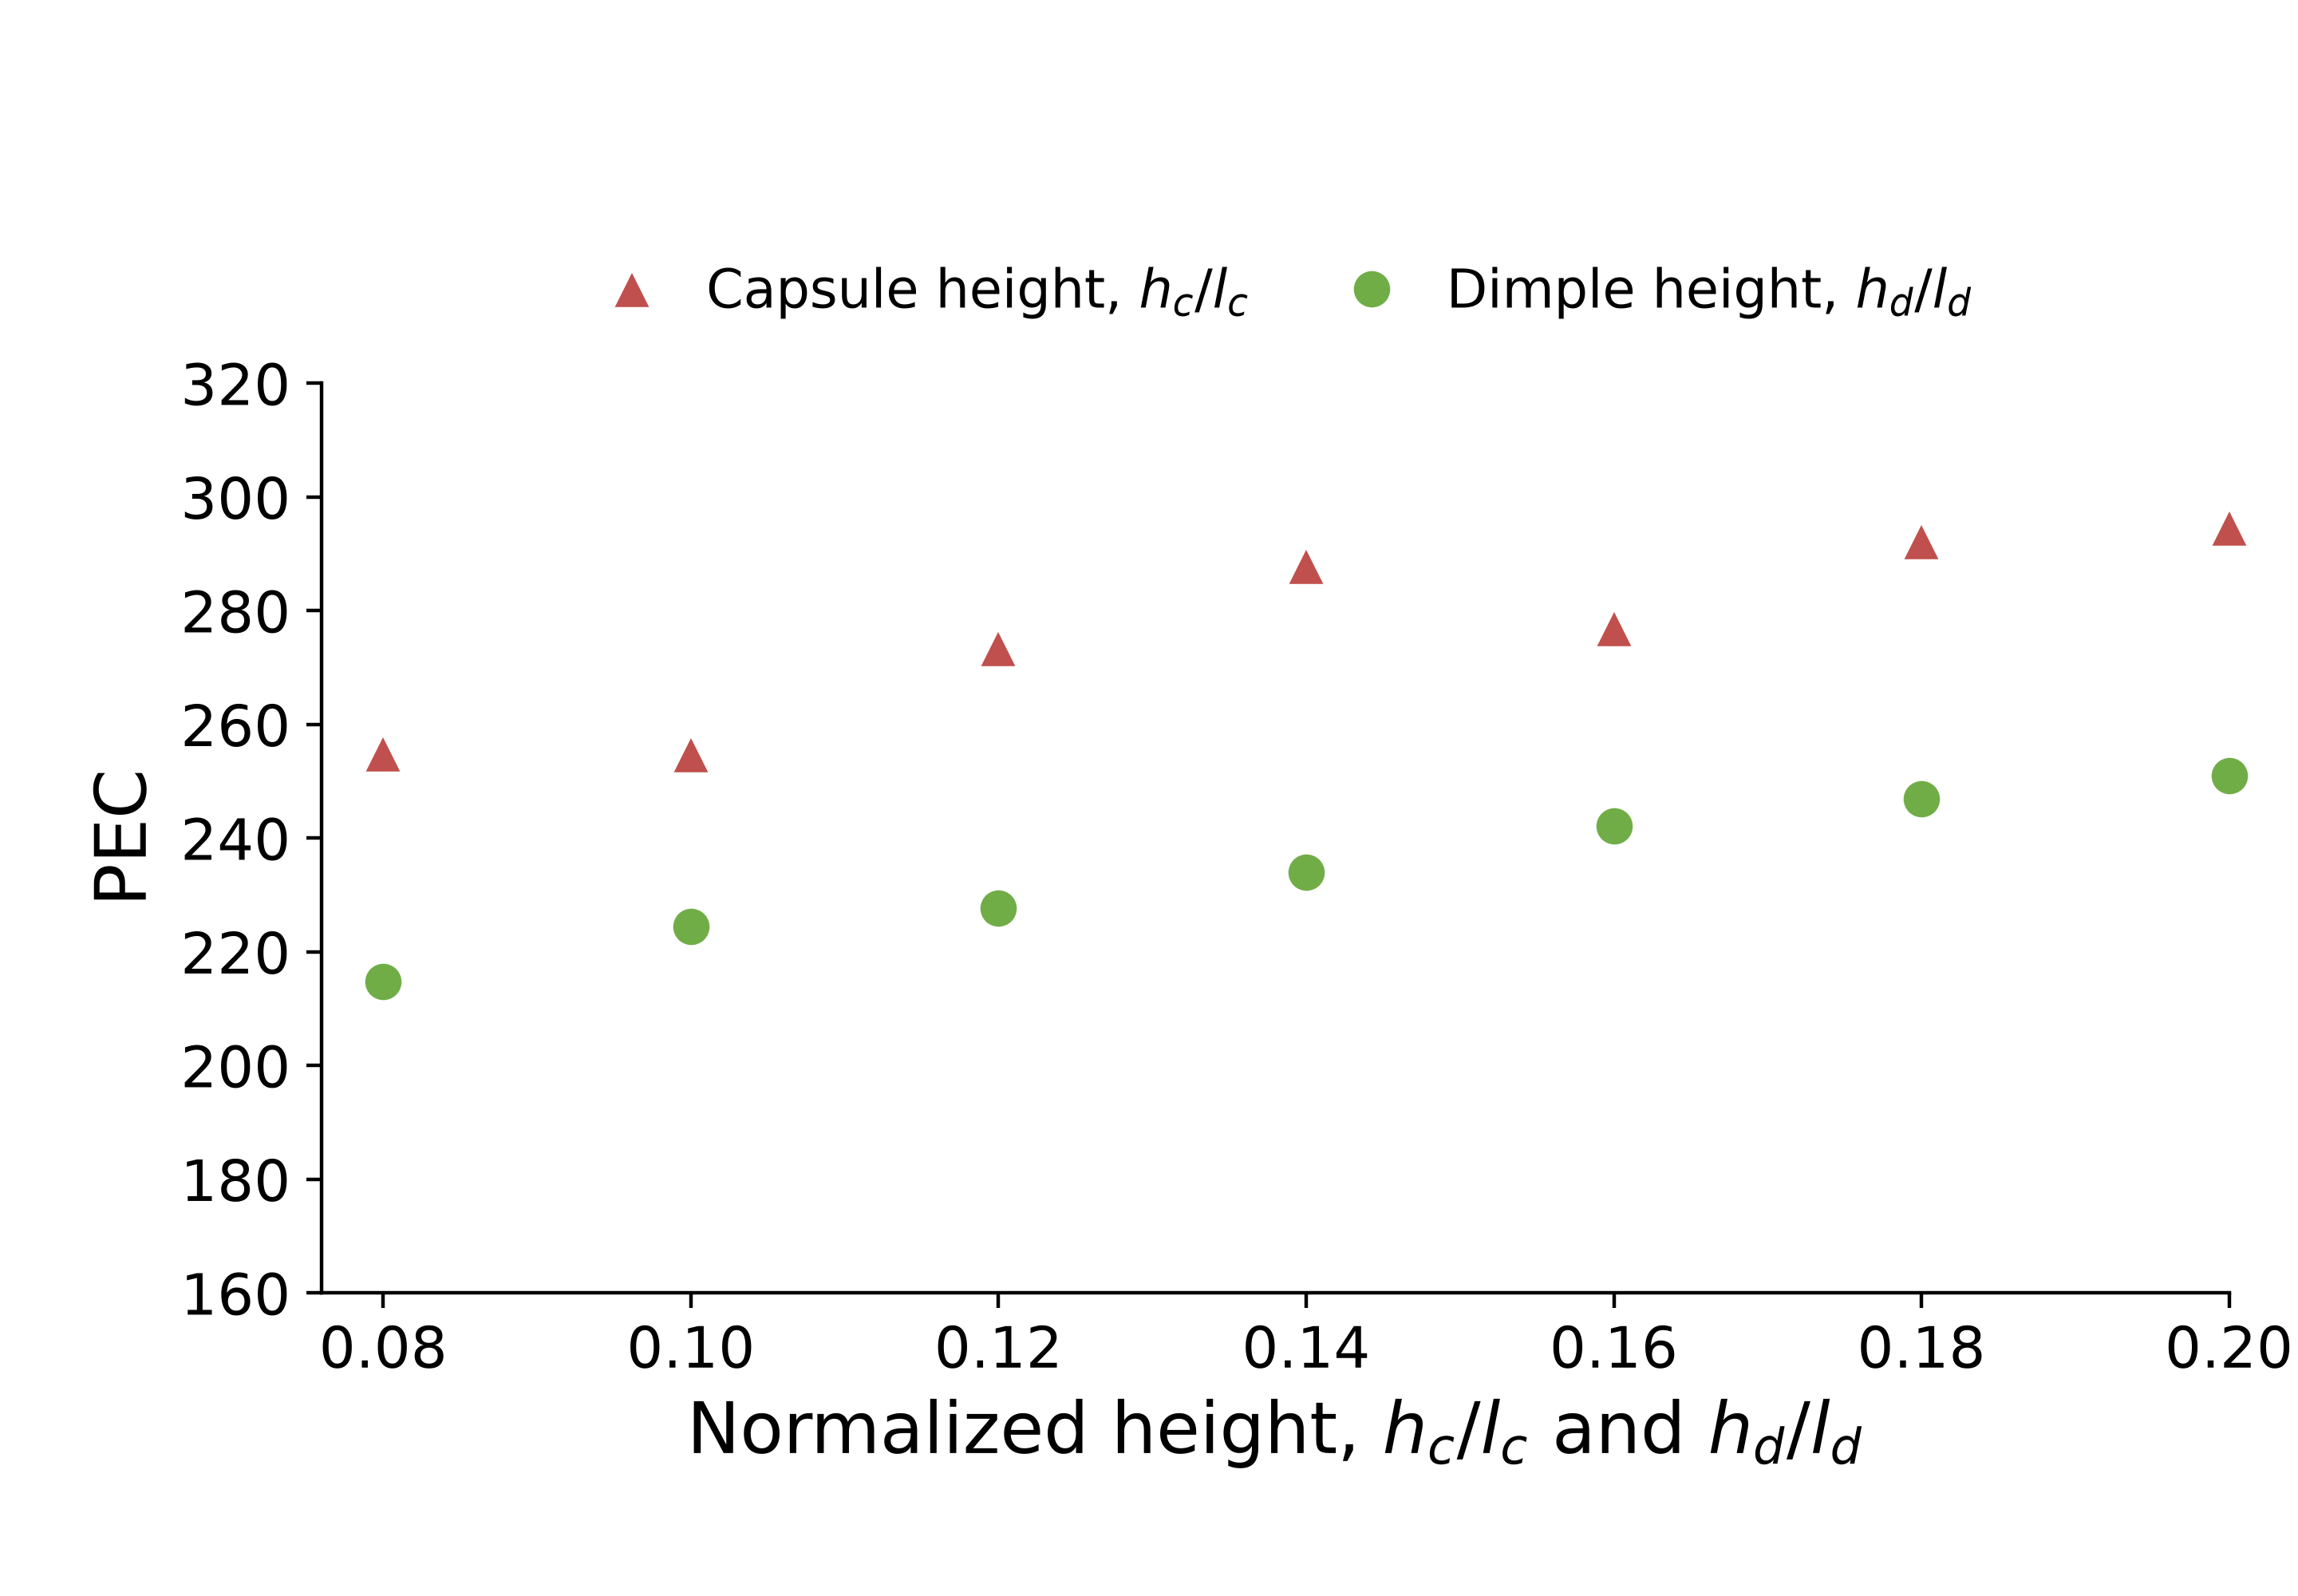
\includegraphics[
        width=\linewidth,
        keepaspectratio,
        interpolate=true
    ]{media/Figure14_PEC_height.png}
    \captionsetup{hypcap=false}
    \captionof{figure}{Two-wall PEC referenced to the fluid-domain mass-average temperature for the height sweeps: $\theta_c=22.5\degree$ and $\theta_d=0\degree$.}
    \label{figure14}
\end{minipage}%

\par\vspace{\baselineskip}

To quantify the paired separation in Figures~\ref{figure13} and~\ref{figure14}, the matched-case PEC difference is defined as
\begin{equation}
  \Delta\mathrm{PEC}=\mathrm{PEC}_{\mathrm{CPHE}}-\mathrm{PEC}_{\mathrm{DPHE}},
  \label{eq:delta-pec}
\end{equation}
where positive values indicate higher CPHE performance. For the seven matched numerical angles, least-squares regression gives
\begin{equation}
  \Delta\mathrm{PEC}_{\theta}=27.76-0.7505\left(\frac{\theta}{1\degree}\right),
  \qquad 0\degree\leq\theta\leq45\degree,
  \label{eq:delta-pec-angle}
\end{equation}
with $R^2=0.889$ and an RMSE of 3.97. The measured difference narrows from 35.06 at $0\degree$ to $-4.79$ at $45\degree$, where DPHE is slightly higher. Figure~\ref{figure14} does not support an analogous height-dependent correlation: for the seven matched normalized heights, $h_c/l_c=h_d/l_d=0.08$--$0.20$, $\Delta\mathrm{PEC}_h$ remains positive but scattered, with a mean of 42.87, a standard deviation of 9.44, and a range of 31.31--59.60; the linear height fit has only $R^2=0.300$. Equation~\eqref{eq:delta-pec-angle} is therefore an empirical benchmark for the angle sweep, while the height result is reported as a descriptive offset rather than a predictive correlation.

These results are limited to the present one-factor sweeps at $\mathrm{Re}=4282$: the angle comparison pairs the CPHE cases at $h_c=2.5$~mm with the DPHE cases at $h_d=3.5$~mm, and the height comparison pairs the CPHE cases at $\theta_c=22.5\degree$ with the DPHE cases at $\theta_d=0\degree$. They do not describe angle--height interactions and should not be extrapolated to other Reynolds numbers, unit-cell geometries, fluids, or boundary conditions.

\begin{figure}[!ht]
  \centering
  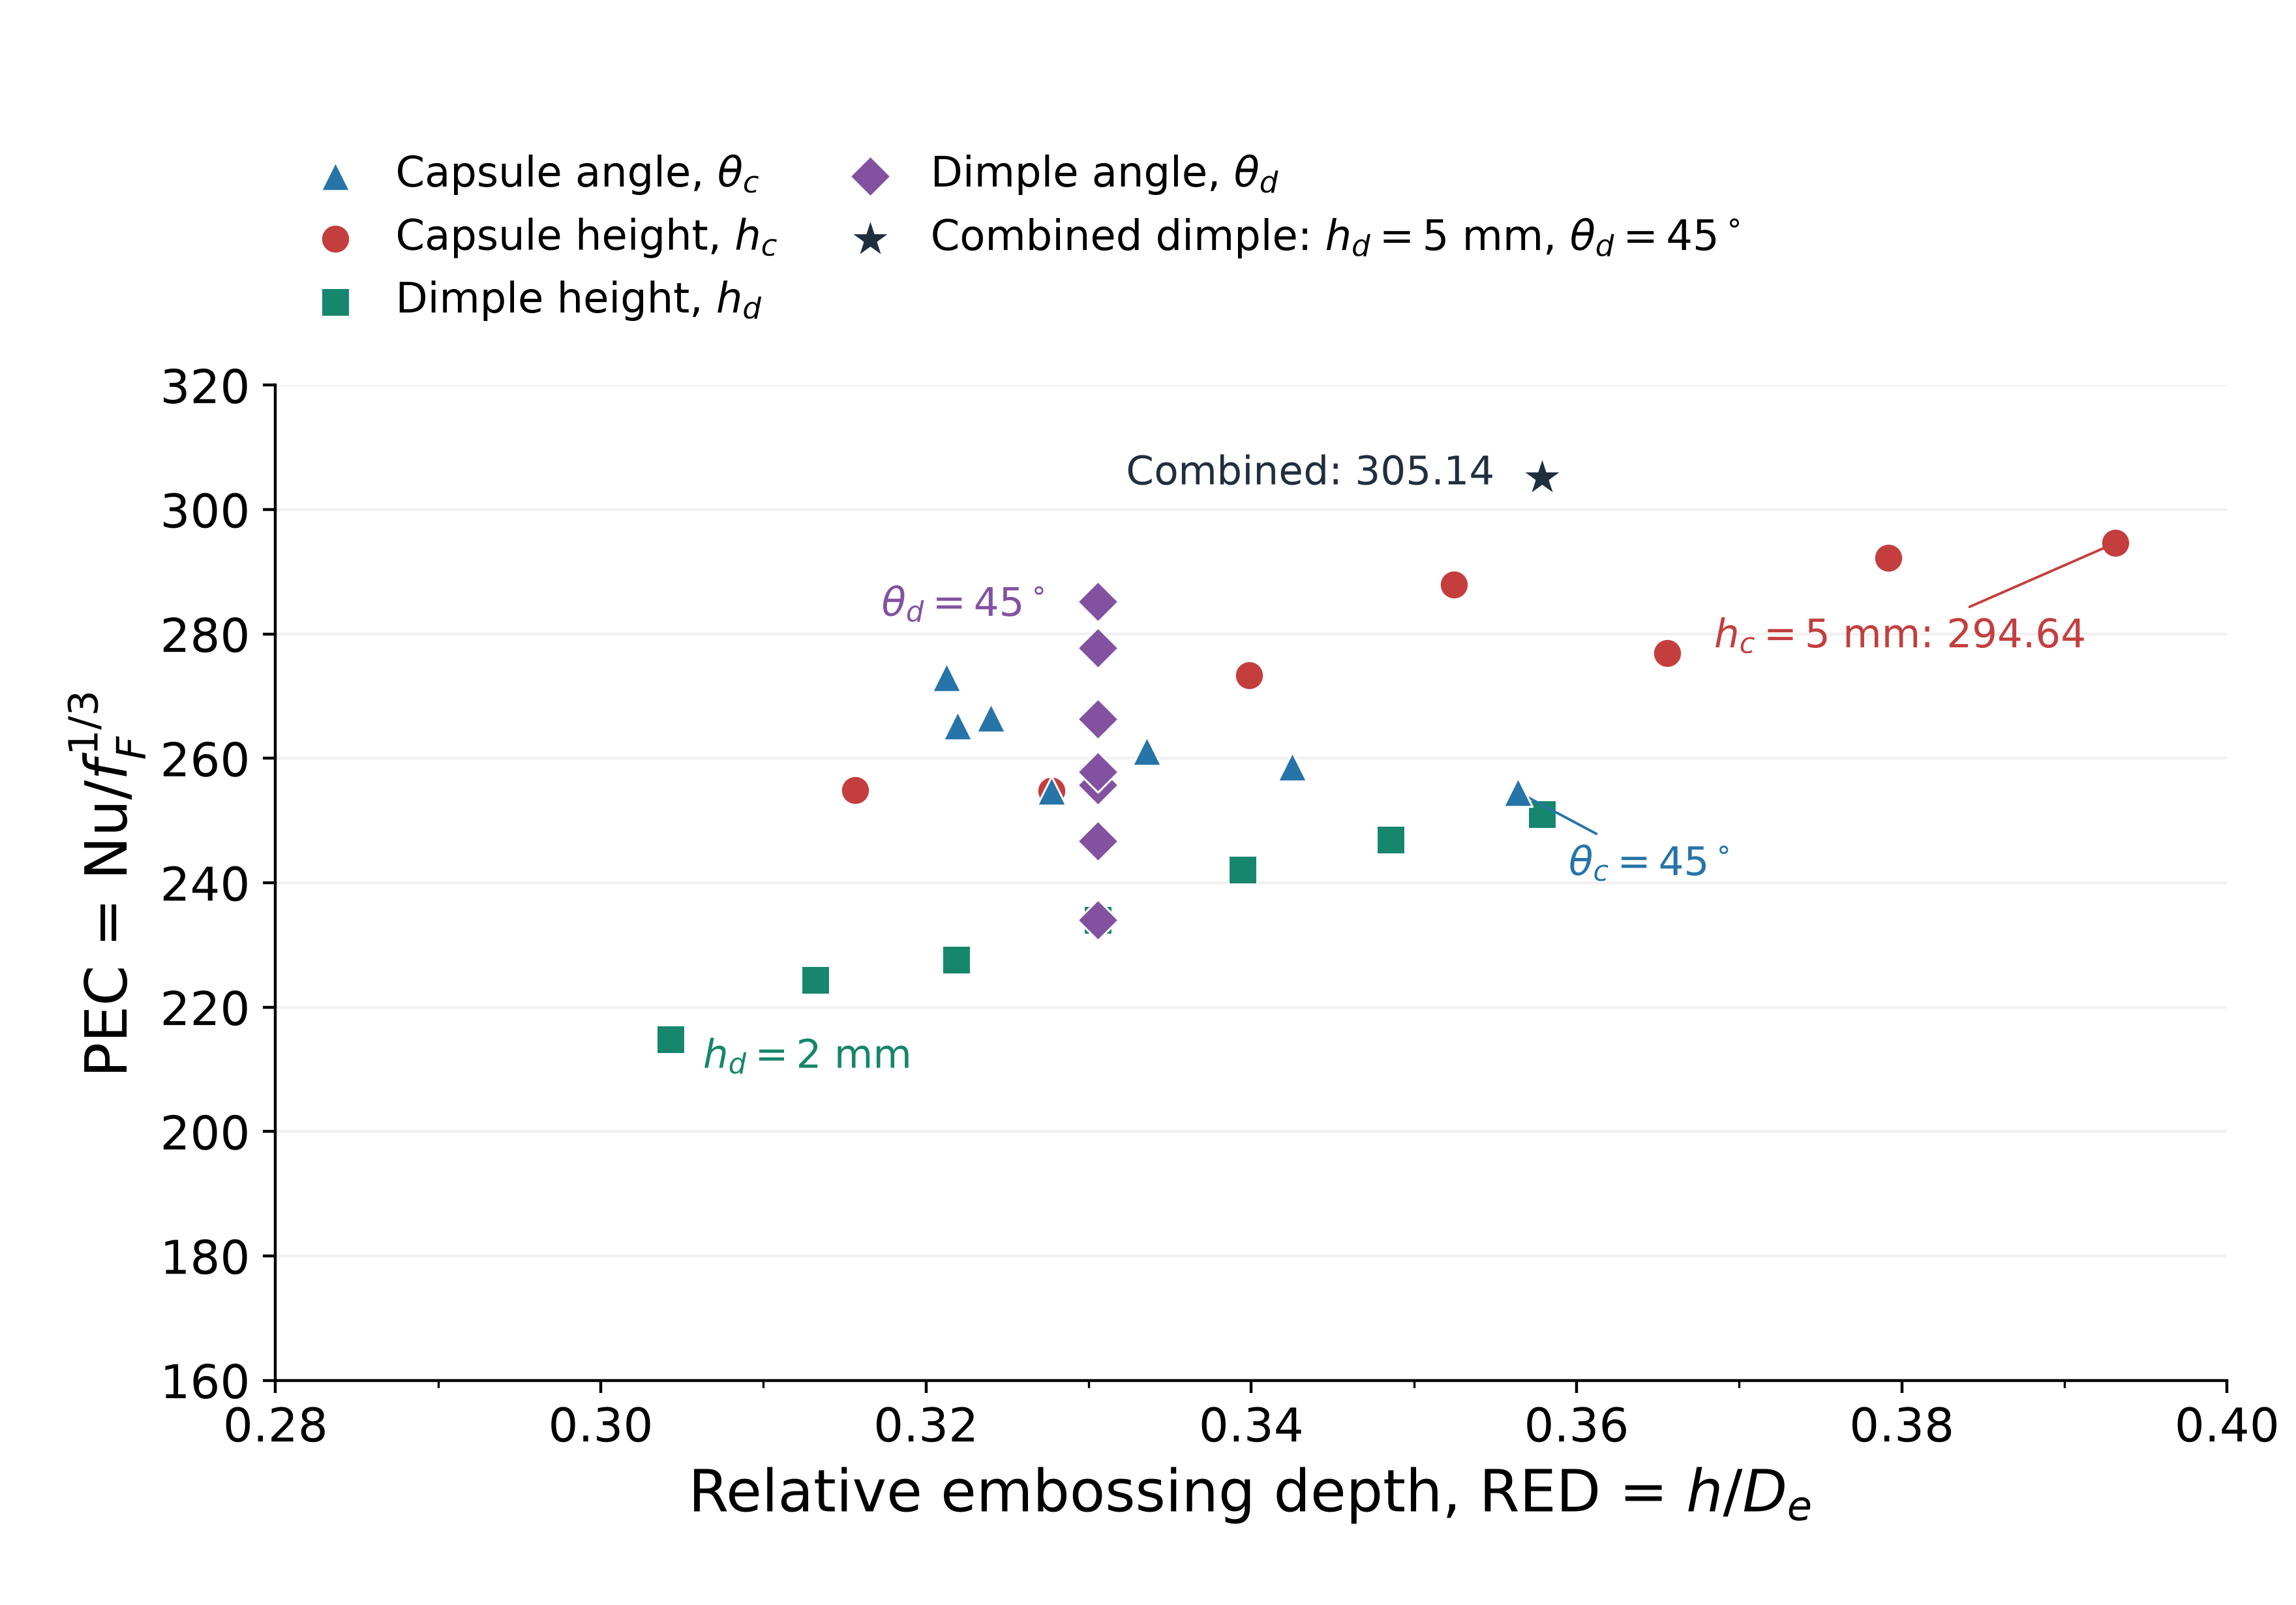
\includegraphics[
    width=0.90\linewidth,
    keepaspectratio,
    interpolate=true
  ]{media/PEC_Vs_RED.png}
  \caption{Performance evaluation criterion (PEC\,=\,Nu/$f^{1/3}$) versus Relative Embossing Depth (\texorpdfstring{RED\,=\,$h/D_e$}{RED = h/De}) for the 28 one-factor cases and the targeted combined dimple case. Markers identify the four parameter families; the star marks $\theta_d=45\degree$ combined with $h_d=5.0$~mm.}
  \label{figure15}
\end{figure}


Higher PEC denotes a better heat-transfer--friction trade-off, so the goal of Figure~\ref{figure15} is to identify the highest PEC within the tested cases. The red $h_c=5.0$~mm point is the best overall result (PEC\,=\,277.1), followed by $h_c=4.5$~mm (PEC\,=\,273.1). The height sweeps extend across RED, whereas the angle sweeps remain at nearly constant RED because their embossing heights are fixed. Dimple-height PEC increases from 186.8 to 237.6, but the larger friction penalty offsets part of the heat-transfer gain. Capsule angle occupies the narrowest PEC band, 244.4--254.8, and provides no clear orientation for a targeted capsule interaction case. Dimple angle spans 219.8--255.1; its high PEC at $\theta_d=45\degree$ follows the sharp reduction in $f$ discussed in Section~\ref{sec:disc_dimple_angle}, not a change in RED. Combining this orientation with $h_d=5.0$~mm produces RED\,=\,357.9, Nu\,=\,77.75, $f=0.0235$, and PEC\,=\,271.5. This is the best tested dimple result and ranks third overall, but the single combined case does not establish a global optimum over height and angle.

\subsection{Limitations of this study}
\label{sec:limitations}

Exploring the intricacies of heat exchanger designs through numerical investigations can be incredibly enlightening, yet it is important to remember these methods are not without their flaws. Recognizing these limitations helps us better understand the results and spot areas that need more research and real-world testing.

For instance, our study assumes that the working fluid does not compress, making the calculations simpler. However, this assumption does not hold up for all real-world scenarios, especially when dealing with gases or other compressible fluids. Additionally, our simulations only consider single-phase flow, meaning they do not take into account the complexities that come with multiphase flows like liquid-gas, or solid-liquid. These interactions can drastically change heat transfer and pressure drops. Moreover, the boundary conditions we apply in simulations tend to be idealized. They do not always reflect the varied and sometimes chaotic conditions found in real-life operations, such as changing inlet temperatures or pressures, and leakage or local geometry variations. We also assume that the physical properties of the working fluid, like density, viscosity, and thermal conductivity, remain constant. In reality, these properties can change significantly with temperature and pressure, which affects both flow and heat transfer.

While our numerical results offer valuable insights, it is crucial to validate them with experimental data to ensure they are accurate and reliable. Unfortunately, finding experimental data for specific configurations and conditions can be a challenge, which can slow down the validation process.


\section{Conclusions}
\label{sec:conclusion}

This study compared 28 one-factor capsule-type (CPHE) and dimple-type (DPHE) unit-cell cases and one targeted combined dimple case under steady-state RANS conditions. Four geometric variables were examined: capsule angle ($\theta_c$), capsule height ($h_c$), dimple height ($h_d$), and dimple angle ($\theta_d$). Nu, $f$, temperature distribution, and flow and vortex characteristics among the parameter families were analyzed; RED and PEC supported comparison across the four parameter families.

Across the tested ranges, capsule angle produced the narrowest PEC variation, spanning 244.4–254.8. Capsule height had a stronger effect, with PEC spanning 244.4–277.1 and the two highest individual values occurring at \(h_c=5.0\) and 4.5 mm. The dimple-angle and dimple-height sweeps covered wider ranges of 219.8–255.1 and 186.8–237.6, respectively. These results indicate greater sensitivity of DPHE performance to the tested geometric parameters, particularly dimple height, but also a greater penalty for unfavourable configurations.

For the matched numerical-angle cases, the CPHE--DPHE difference follows $\Delta\mathrm{PEC}_{\theta}=27.76-0.7505(\theta/1\degree)$ with $R^2=0.889$ over $0\degree$--$45\degree$. The matched normalized-height differences remain positive but do not support a comparable height-dependent correlation, averaging 42.87 across $h/l=0.08$--$0.20$. Both comparisons are empirical descriptors of the tested one-factor cases at $\mathrm{Re}=4282$.

Among the tested dimple geometries, the targeted combination $\theta_d=45\degree$ and $h_d=5.0$~mm gave the highest PEC (271.5). This value is 6.4\% above the corresponding $h_d=3.5$~mm angle-sweep case and 14.3\% above the corresponding $\theta_d=0\degree$, $h_d=5.0$~mm height-sweep case. It is therefore the best-performing tested dimple configuration and ranks third overall, behind the two leading capsule-height cases. Because only one combined dimple interaction case was evaluated, this result does not establish a global optimum. The conclusions remain specific to the tested unit-cell conditions; experimental validation and tests at additional Reynolds numbers, heights, angles, and fluids are required.



\authorcontributions{Both C.S.C. and C.S. have similar contributions to the paper and are acknowledged as the first authors. Conceptualization, S.V. and L.S.; methodology, S.V., K.I., A.D. and J.T.; software, C.S.C. and C.S.; formal analysis, C.S.C. and C.S.; investigation, C.S.C. and C.S.; resources, L.S.; data curation, C.S.C. and C.S.; writing: original draft preparation, C.S.C. and C.S.; writing: review and editing, S.V. and K.I.; visualization, C.S.C. and C.S.; supervision, L.S., S.V., K.I., J.T, and A.D.; project administration, S.V.. All authors have read and agreed to the submitted version of the manuscript.}

\funding{This research received no external funding}

\institutionalreview{Not applicable}

\informedconsent{Not applicable}

\dataavailability{The data presented in this study are available on request from the corresponding author}

\acknowledgments{InKorr Pty Ltd. provided resources for this research}

\conflictsofinterest{The authors declare no conflicts of interest}

\useofartificialintelligence{AI or AI-assisted tools were not used in drafting any aspect of this manuscript}

% Keep references aligned with the local review margins.
\reftitle{References}
\bibliography{references}
\PublishersNote{}
\end{document}
